% Options for packages loaded elsewhere
\PassOptionsToPackage{unicode}{hyperref}
\PassOptionsToPackage{hyphens}{url}
%
\documentclass[
]{article}
\usepackage{lmodern}
\usepackage{amssymb,amsmath}
\usepackage{ifxetex,ifluatex}
\ifnum 0\ifxetex 1\fi\ifluatex 1\fi=0 % if pdftex
  \usepackage[T1]{fontenc}
  \usepackage[utf8]{inputenc}
  \usepackage{textcomp} % provide euro and other symbols
\else % if luatex or xetex
  \usepackage{unicode-math}
  \defaultfontfeatures{Scale=MatchLowercase}
  \defaultfontfeatures[\rmfamily]{Ligatures=TeX,Scale=1}
\fi
% Use upquote if available, for straight quotes in verbatim environments
\IfFileExists{upquote.sty}{\usepackage{upquote}}{}
\IfFileExists{microtype.sty}{% use microtype if available
  \usepackage[]{microtype}
  \UseMicrotypeSet[protrusion]{basicmath} % disable protrusion for tt fonts
}{}
\makeatletter
\@ifundefined{KOMAClassName}{% if non-KOMA class
  \IfFileExists{parskip.sty}{%
    \usepackage{parskip}
  }{% else
    \setlength{\parindent}{0pt}
    \setlength{\parskip}{6pt plus 2pt minus 1pt}}
}{% if KOMA class
  \KOMAoptions{parskip=half}}
\makeatother
\usepackage{xcolor}
\IfFileExists{xurl.sty}{\usepackage{xurl}}{} % add URL line breaks if available
\IfFileExists{bookmark.sty}{\usepackage{bookmark}}{\usepackage{hyperref}}
\hypersetup{
  pdftitle={Statistical Learning Project},
  hidelinks,
  pdfcreator={LaTeX via pandoc}}
\urlstyle{same} % disable monospaced font for URLs
\usepackage[margin=1in]{geometry}
\usepackage{color}
\usepackage{fancyvrb}
\newcommand{\VerbBar}{|}
\newcommand{\VERB}{\Verb[commandchars=\\\{\}]}
\DefineVerbatimEnvironment{Highlighting}{Verbatim}{commandchars=\\\{\}}
% Add ',fontsize=\small' for more characters per line
\usepackage{framed}
\definecolor{shadecolor}{RGB}{248,248,248}
\newenvironment{Shaded}{\begin{snugshade}}{\end{snugshade}}
\newcommand{\AlertTok}[1]{\textcolor[rgb]{0.94,0.16,0.16}{#1}}
\newcommand{\AnnotationTok}[1]{\textcolor[rgb]{0.56,0.35,0.01}{\textbf{\textit{#1}}}}
\newcommand{\AttributeTok}[1]{\textcolor[rgb]{0.77,0.63,0.00}{#1}}
\newcommand{\BaseNTok}[1]{\textcolor[rgb]{0.00,0.00,0.81}{#1}}
\newcommand{\BuiltInTok}[1]{#1}
\newcommand{\CharTok}[1]{\textcolor[rgb]{0.31,0.60,0.02}{#1}}
\newcommand{\CommentTok}[1]{\textcolor[rgb]{0.56,0.35,0.01}{\textit{#1}}}
\newcommand{\CommentVarTok}[1]{\textcolor[rgb]{0.56,0.35,0.01}{\textbf{\textit{#1}}}}
\newcommand{\ConstantTok}[1]{\textcolor[rgb]{0.00,0.00,0.00}{#1}}
\newcommand{\ControlFlowTok}[1]{\textcolor[rgb]{0.13,0.29,0.53}{\textbf{#1}}}
\newcommand{\DataTypeTok}[1]{\textcolor[rgb]{0.13,0.29,0.53}{#1}}
\newcommand{\DecValTok}[1]{\textcolor[rgb]{0.00,0.00,0.81}{#1}}
\newcommand{\DocumentationTok}[1]{\textcolor[rgb]{0.56,0.35,0.01}{\textbf{\textit{#1}}}}
\newcommand{\ErrorTok}[1]{\textcolor[rgb]{0.64,0.00,0.00}{\textbf{#1}}}
\newcommand{\ExtensionTok}[1]{#1}
\newcommand{\FloatTok}[1]{\textcolor[rgb]{0.00,0.00,0.81}{#1}}
\newcommand{\FunctionTok}[1]{\textcolor[rgb]{0.00,0.00,0.00}{#1}}
\newcommand{\ImportTok}[1]{#1}
\newcommand{\InformationTok}[1]{\textcolor[rgb]{0.56,0.35,0.01}{\textbf{\textit{#1}}}}
\newcommand{\KeywordTok}[1]{\textcolor[rgb]{0.13,0.29,0.53}{\textbf{#1}}}
\newcommand{\NormalTok}[1]{#1}
\newcommand{\OperatorTok}[1]{\textcolor[rgb]{0.81,0.36,0.00}{\textbf{#1}}}
\newcommand{\OtherTok}[1]{\textcolor[rgb]{0.56,0.35,0.01}{#1}}
\newcommand{\PreprocessorTok}[1]{\textcolor[rgb]{0.56,0.35,0.01}{\textit{#1}}}
\newcommand{\RegionMarkerTok}[1]{#1}
\newcommand{\SpecialCharTok}[1]{\textcolor[rgb]{0.00,0.00,0.00}{#1}}
\newcommand{\SpecialStringTok}[1]{\textcolor[rgb]{0.31,0.60,0.02}{#1}}
\newcommand{\StringTok}[1]{\textcolor[rgb]{0.31,0.60,0.02}{#1}}
\newcommand{\VariableTok}[1]{\textcolor[rgb]{0.00,0.00,0.00}{#1}}
\newcommand{\VerbatimStringTok}[1]{\textcolor[rgb]{0.31,0.60,0.02}{#1}}
\newcommand{\WarningTok}[1]{\textcolor[rgb]{0.56,0.35,0.01}{\textbf{\textit{#1}}}}
\usepackage{graphicx,grffile}
\makeatletter
\def\maxwidth{\ifdim\Gin@nat@width>\linewidth\linewidth\else\Gin@nat@width\fi}
\def\maxheight{\ifdim\Gin@nat@height>\textheight\textheight\else\Gin@nat@height\fi}
\makeatother
% Scale images if necessary, so that they will not overflow the page
% margins by default, and it is still possible to overwrite the defaults
% using explicit options in \includegraphics[width, height, ...]{}
\setkeys{Gin}{width=\maxwidth,height=\maxheight,keepaspectratio}
% Set default figure placement to htbp
\makeatletter
\def\fps@figure{htbp}
\makeatother
\setlength{\emergencystretch}{3em} % prevent overfull lines
\providecommand{\tightlist}{%
  \setlength{\itemsep}{0pt}\setlength{\parskip}{0pt}}
\setcounter{secnumdepth}{-\maxdimen} % remove section numbering
\usepackage{booktabs}
\usepackage{longtable}
\usepackage{array}
\usepackage{multirow}
\usepackage{wrapfig}
\usepackage{float}
\usepackage{colortbl}
\usepackage{pdflscape}
\usepackage{tabu}
\usepackage{threeparttable}
\usepackage{threeparttablex}
\usepackage[normalem]{ulem}
\usepackage{makecell}
\usepackage{xcolor}

\title{Statistical Learning Project}
\author{}
\date{\vspace{-2.5em}}

\begin{document}
\maketitle

{
\setcounter{tocdepth}{2}
\tableofcontents
}
~\\

Author: Andrea Ierardi

~\\

Repository : Code
\href{https://github.com/Andreaierardi/Statistical-Learning-Project}{link}

~\\

\hypertarget{assignment}{%
\subsubsection{Assignment}\label{assignment}}

The exam consists in two assignments, one on the first part(regression,
tree, neural nets) and the second part (unsupervised learning). For both
you must prepare a writing report using one or more techniques and
comparing their performance on one or more data set chosen by the
student.

~\\

\hypertarget{libraries}{%
\section{Libraries}\label{libraries}}

\begin{Shaded}
\begin{Highlighting}[]
\KeywordTok{library}\NormalTok{(knitr)}
\KeywordTok{library}\NormalTok{(ggplot2)}
\KeywordTok{library}\NormalTok{(plotly)}
\end{Highlighting}
\end{Shaded}

\begin{verbatim}
## 
## Attaching package: 'plotly'
\end{verbatim}

\begin{verbatim}
## The following object is masked from 'package:ggplot2':
## 
##     last_plot
\end{verbatim}

\begin{verbatim}
## The following object is masked from 'package:stats':
## 
##     filter
\end{verbatim}

\begin{verbatim}
## The following object is masked from 'package:graphics':
## 
##     layout
\end{verbatim}

\begin{Shaded}
\begin{Highlighting}[]
\KeywordTok{library}\NormalTok{(tidyr)}
\KeywordTok{library}\NormalTok{(dplyr)}
\end{Highlighting}
\end{Shaded}

\begin{verbatim}
## 
## Attaching package: 'dplyr'
\end{verbatim}

\begin{verbatim}
## The following objects are masked from 'package:stats':
## 
##     filter, lag
\end{verbatim}

\begin{verbatim}
## The following objects are masked from 'package:base':
## 
##     intersect, setdiff, setequal, union
\end{verbatim}

\begin{Shaded}
\begin{Highlighting}[]
\KeywordTok{library}\NormalTok{(png)}
\KeywordTok{library}\NormalTok{(ggpubr)}
\KeywordTok{library}\NormalTok{(tidyverse)}
\end{Highlighting}
\end{Shaded}

\begin{verbatim}
## -- Attaching packages -------------------------------------------------------------------------------------------- tidyverse 1.3.0 --
\end{verbatim}

\begin{verbatim}
## v tibble  3.0.2     v stringr 1.4.0
## v readr   1.3.1     v forcats 0.5.0
## v purrr   0.3.4
\end{verbatim}

\begin{verbatim}
## -- Conflicts ----------------------------------------------------------------------------------------------- tidyverse_conflicts() --
## x dplyr::filter() masks plotly::filter(), stats::filter()
## x dplyr::lag()    masks stats::lag()
\end{verbatim}

\begin{Shaded}
\begin{Highlighting}[]
\KeywordTok{library}\NormalTok{(caTools)}
\KeywordTok{library}\NormalTok{(caret)}
\end{Highlighting}
\end{Shaded}

\begin{verbatim}
## Loading required package: lattice
\end{verbatim}

\begin{verbatim}
## 
## Attaching package: 'caret'
\end{verbatim}

\begin{verbatim}
## The following object is masked from 'package:purrr':
## 
##     lift
\end{verbatim}

\begin{Shaded}
\begin{Highlighting}[]
\KeywordTok{library}\NormalTok{(tree)}
\end{Highlighting}
\end{Shaded}

\begin{verbatim}
## Registered S3 method overwritten by 'tree':
##   method     from
##   print.tree cli
\end{verbatim}

\begin{Shaded}
\begin{Highlighting}[]
\KeywordTok{library}\NormalTok{(MASS)}
\end{Highlighting}
\end{Shaded}

\begin{verbatim}
## 
## Attaching package: 'MASS'
\end{verbatim}

\begin{verbatim}
## The following object is masked from 'package:dplyr':
## 
##     select
\end{verbatim}

\begin{verbatim}
## The following object is masked from 'package:plotly':
## 
##     select
\end{verbatim}

\begin{Shaded}
\begin{Highlighting}[]
\KeywordTok{library}\NormalTok{(randomForest)}
\end{Highlighting}
\end{Shaded}

\begin{verbatim}
## randomForest 4.6-14
\end{verbatim}

\begin{verbatim}
## Type rfNews() to see new features/changes/bug fixes.
\end{verbatim}

\begin{verbatim}
## 
## Attaching package: 'randomForest'
\end{verbatim}

\begin{verbatim}
## The following object is masked from 'package:dplyr':
## 
##     combine
\end{verbatim}

\begin{verbatim}
## The following object is masked from 'package:ggplot2':
## 
##     margin
\end{verbatim}

\begin{Shaded}
\begin{Highlighting}[]
\KeywordTok{library}\NormalTok{(ranger)}
\end{Highlighting}
\end{Shaded}

\begin{verbatim}
## 
## Attaching package: 'ranger'
\end{verbatim}

\begin{verbatim}
## The following object is masked from 'package:randomForest':
## 
##     importance
\end{verbatim}

\begin{Shaded}
\begin{Highlighting}[]
\KeywordTok{library}\NormalTok{(tuneRanger)}
\end{Highlighting}
\end{Shaded}

\begin{verbatim}
## Loading required package: mlrMBO
\end{verbatim}

\begin{verbatim}
## Loading required package: mlr
\end{verbatim}

\begin{verbatim}
## Loading required package: ParamHelpers
\end{verbatim}

\begin{verbatim}
## 'mlr' is in maintenance mode since July 2019. Future development
## efforts will go into its successor 'mlr3' (<https://mlr3.mlr-org.com>).
\end{verbatim}

\begin{verbatim}
## 
## Attaching package: 'mlr'
\end{verbatim}

\begin{verbatim}
## The following object is masked from 'package:caret':
## 
##     train
\end{verbatim}

\begin{verbatim}
## Loading required package: smoof
\end{verbatim}

\begin{verbatim}
## Loading required package: checkmate
\end{verbatim}

\begin{verbatim}
## Loading required package: parallel
\end{verbatim}

\begin{verbatim}
## Loading required package: lubridate
\end{verbatim}

\begin{verbatim}
## 
## Attaching package: 'lubridate'
\end{verbatim}

\begin{verbatim}
## The following objects are masked from 'package:base':
## 
##     date, intersect, setdiff, union
\end{verbatim}

\begin{verbatim}
## Loading required package: lhs
\end{verbatim}

\begin{Shaded}
\begin{Highlighting}[]
\KeywordTok{library}\NormalTok{(keras)}

\KeywordTok{library}\NormalTok{(kableExtra)}
\end{Highlighting}
\end{Shaded}

\begin{verbatim}
## 
## Attaching package: 'kableExtra'
\end{verbatim}

\begin{verbatim}
## The following object is masked from 'package:dplyr':
## 
##     group_rows
\end{verbatim}

\begin{Shaded}
\begin{Highlighting}[]
\KeywordTok{library}\NormalTok{(clustMixType)}
\KeywordTok{library}\NormalTok{(cluster)}
\KeywordTok{library}\NormalTok{(dendextend) }
\end{Highlighting}
\end{Shaded}

\begin{verbatim}
## 
## ---------------------
## Welcome to dendextend version 1.13.4
## Type citation('dendextend') for how to cite the package.
## 
## Type browseVignettes(package = 'dendextend') for the package vignette.
## The github page is: https://github.com/talgalili/dendextend/
## 
## Suggestions and bug-reports can be submitted at: https://github.com/talgalili/dendextend/issues
## Or contact: <tal.galili@gmail.com>
## 
##  To suppress this message use:  suppressPackageStartupMessages(library(dendextend))
## ---------------------
\end{verbatim}

\begin{verbatim}
## 
## Attaching package: 'dendextend'
\end{verbatim}

\begin{verbatim}
## The following object is masked from 'package:ggpubr':
## 
##     rotate
\end{verbatim}

\begin{verbatim}
## The following object is masked from 'package:stats':
## 
##     cutree
\end{verbatim}

\begin{Shaded}
\begin{Highlighting}[]
\KeywordTok{library}\NormalTok{(readr)}

\KeywordTok{library}\NormalTok{(factoextra)}
\end{Highlighting}
\end{Shaded}

\begin{verbatim}
## Welcome! Want to learn more? See two factoextra-related books at https://goo.gl/ve3WBa
\end{verbatim}

\begin{Shaded}
\begin{Highlighting}[]
\KeywordTok{library}\NormalTok{(FactoMineR)}


\KeywordTok{library}\NormalTok{(PCAmixdata)}
\end{Highlighting}
\end{Shaded}

~\\

\hypertarget{dataset}{%
\section{Dataset}\label{dataset}}

Link of the
\href{https://www.kaggle.com/dgomonov/new-york-city-airbnb-open-data}{dataset}

\begin{Shaded}
\begin{Highlighting}[]
\NormalTok{ds =}\StringTok{ }\KeywordTok{read.csv}\NormalTok{(}\StringTok{"AB_NYC_2019.csv"}\NormalTok{)}
\end{Highlighting}
\end{Shaded}

~\\

\hypertarget{data-inspection}{%
\section{Data Inspection}\label{data-inspection}}

\begin{Shaded}
\begin{Highlighting}[]
\KeywordTok{head}\NormalTok{(ds)}
\end{Highlighting}
\end{Shaded}

\begin{verbatim}
##     id                                             name host_id   host_name
## 1 2539               Clean & quiet apt home by the park    2787        John
## 2 2595                            Skylit Midtown Castle    2845    Jennifer
## 3 3647              THE VILLAGE OF HARLEM....NEW YORK !    4632   Elisabeth
## 4 3831                  Cozy Entire Floor of Brownstone    4869 LisaRoxanne
## 5 5022 Entire Apt: Spacious Studio/Loft by central park    7192       Laura
## 6 5099        Large Cozy 1 BR Apartment In Midtown East    7322       Chris
##   neighbourhood_group neighbourhood latitude longitude       room_type price
## 1            Brooklyn    Kensington 40.64749 -73.97237    Private room   149
## 2           Manhattan       Midtown 40.75362 -73.98377 Entire home/apt   225
## 3           Manhattan        Harlem 40.80902 -73.94190    Private room   150
## 4            Brooklyn  Clinton Hill 40.68514 -73.95976 Entire home/apt    89
## 5           Manhattan   East Harlem 40.79851 -73.94399 Entire home/apt    80
## 6           Manhattan   Murray Hill 40.74767 -73.97500 Entire home/apt   200
##   minimum_nights number_of_reviews last_review reviews_per_month
## 1              1                 9  2018-10-19              0.21
## 2              1                45  2019-05-21              0.38
## 3              3                 0                            NA
## 4              1               270  2019-07-05              4.64
## 5             10                 9  2018-11-19              0.10
## 6              3                74  2019-06-22              0.59
##   calculated_host_listings_count availability_365
## 1                              6              365
## 2                              2              355
## 3                              1              365
## 4                              1              194
## 5                              1                0
## 6                              1              129
\end{verbatim}

\begin{Shaded}
\begin{Highlighting}[]
\KeywordTok{summary}\NormalTok{(ds)}
\end{Highlighting}
\end{Shaded}

\begin{verbatim}
##        id               name              host_id           host_name        
##  Min.   :    2539   Length:48895       Min.   :     2438   Length:48895      
##  1st Qu.: 9471945   Class :character   1st Qu.:  7822033   Class :character  
##  Median :19677284   Mode  :character   Median : 30793816   Mode  :character  
##  Mean   :19017143                      Mean   : 67620011                     
##  3rd Qu.:29152178                      3rd Qu.:107434423                     
##  Max.   :36487245                      Max.   :274321313                     
##                                                                              
##  neighbourhood_group neighbourhood         latitude       longitude     
##  Length:48895        Length:48895       Min.   :40.50   Min.   :-74.24  
##  Class :character    Class :character   1st Qu.:40.69   1st Qu.:-73.98  
##  Mode  :character    Mode  :character   Median :40.72   Median :-73.96  
##                                         Mean   :40.73   Mean   :-73.95  
##                                         3rd Qu.:40.76   3rd Qu.:-73.94  
##                                         Max.   :40.91   Max.   :-73.71  
##                                                                         
##   room_type             price         minimum_nights    number_of_reviews
##  Length:48895       Min.   :    0.0   Min.   :   1.00   Min.   :  0.00   
##  Class :character   1st Qu.:   69.0   1st Qu.:   1.00   1st Qu.:  1.00   
##  Mode  :character   Median :  106.0   Median :   3.00   Median :  5.00   
##                     Mean   :  152.7   Mean   :   7.03   Mean   : 23.27   
##                     3rd Qu.:  175.0   3rd Qu.:   5.00   3rd Qu.: 24.00   
##                     Max.   :10000.0   Max.   :1250.00   Max.   :629.00   
##                                                                          
##  last_review        reviews_per_month calculated_host_listings_count
##  Length:48895       Min.   : 0.010    Min.   :  1.000               
##  Class :character   1st Qu.: 0.190    1st Qu.:  1.000               
##  Mode  :character   Median : 0.720    Median :  1.000               
##                     Mean   : 1.373    Mean   :  7.144               
##                     3rd Qu.: 2.020    3rd Qu.:  2.000               
##                     Max.   :58.500    Max.   :327.000               
##                     NA's   :10052                                   
##  availability_365
##  Min.   :  0.0   
##  1st Qu.:  0.0   
##  Median : 45.0   
##  Mean   :112.8   
##  3rd Qu.:227.0   
##  Max.   :365.0   
## 
\end{verbatim}

\begin{Shaded}
\begin{Highlighting}[]
\KeywordTok{cat}\NormalTok{(}\StringTok{"Shape of the dataset:"}\NormalTok{ ,}\KeywordTok{dim}\NormalTok{(ds))}
\end{Highlighting}
\end{Shaded}

\begin{verbatim}
## Shape of the dataset: 48895 16
\end{verbatim}

\begin{Shaded}
\begin{Highlighting}[]
\NormalTok{img <-}\StringTok{ }\KeywordTok{readPNG}\NormalTok{(}\StringTok{"map.png"}\NormalTok{)}


\NormalTok{map_ds =}\StringTok{ }\KeywordTok{ggplot}\NormalTok{() }\OperatorTok{+}\StringTok{ }\KeywordTok{background_image}\NormalTok{(img)}\OperatorTok{+}\StringTok{ }\KeywordTok{geom_point}\NormalTok{(}\DataTypeTok{data =}\NormalTok{ ds,  }\KeywordTok{aes}\NormalTok{(}\DataTypeTok{y=}\NormalTok{latitude,}\DataTypeTok{x =}\NormalTok{ longitude, }\DataTypeTok{color =}\NormalTok{ price)) }
\NormalTok{map_ds}
\end{Highlighting}
\end{Shaded}

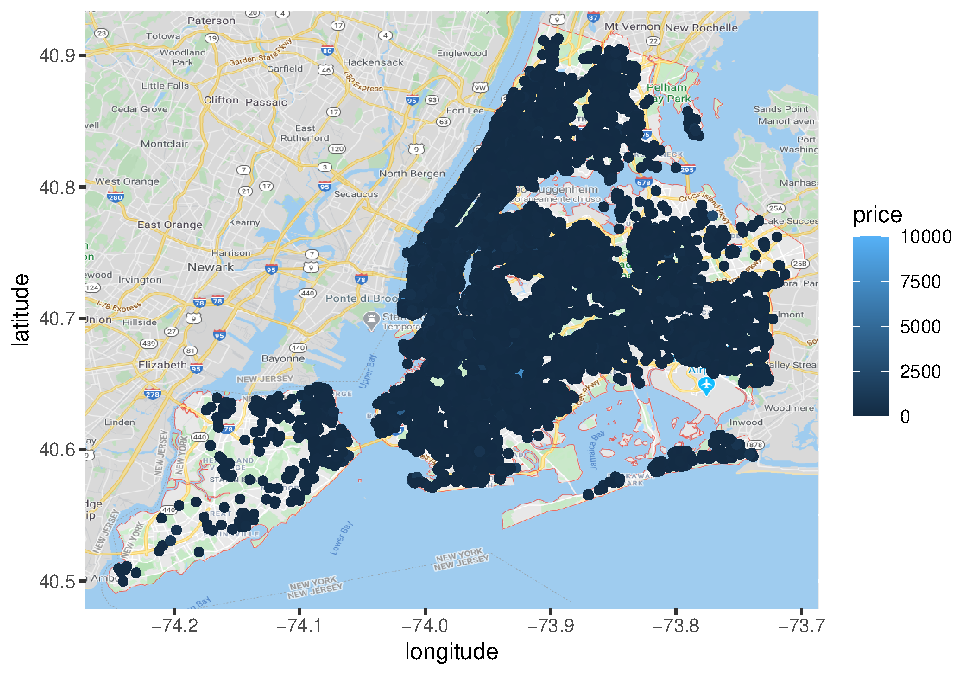
\includegraphics{project-code_files/figure-latex/unnamed-chunk-5-1.pdf}

~~

\hypertarget{data-cleaning}{%
\section{Data cleaning}\label{data-cleaning}}

~\\

\hypertarget{check-for-na-and-null-values}{%
\subsection{Check for NA and NULL
values}\label{check-for-na-and-null-values}}

\begin{Shaded}
\begin{Highlighting}[]
\KeywordTok{apply}\NormalTok{(ds,}\DecValTok{2}\NormalTok{,}\ControlFlowTok{function}\NormalTok{(x) }\KeywordTok{sum}\NormalTok{(}\KeywordTok{is.na}\NormalTok{(x)))}
\end{Highlighting}
\end{Shaded}

\begin{verbatim}
##                             id                           name 
##                              0                              0 
##                        host_id                      host_name 
##                              0                              0 
##            neighbourhood_group                  neighbourhood 
##                              0                              0 
##                       latitude                      longitude 
##                              0                              0 
##                      room_type                          price 
##                              0                              0 
##                 minimum_nights              number_of_reviews 
##                              0                              0 
##                    last_review              reviews_per_month 
##                              0                          10052 
## calculated_host_listings_count               availability_365 
##                              0                              0
\end{verbatim}

~\\

\hypertarget{variable-selection}{%
\subsection{Variable selection}\label{variable-selection}}

\begin{Shaded}
\begin{Highlighting}[]
\NormalTok{dataset =}\StringTok{ }\NormalTok{ds  }\OperatorTok\StringTok{ }\NormalTok{dplyr}\OperatorTok{::}\KeywordTok{select}\NormalTok{(neighbourhood_group,latitude, longitude, room_type,price)}

\KeywordTok{head}\NormalTok{(dataset)}
\end{Highlighting}
\end{Shaded}

\begin{verbatim}
##   neighbourhood_group latitude longitude       room_type price
## 1            Brooklyn 40.64749 -73.97237    Private room   149
## 2           Manhattan 40.75362 -73.98377 Entire home/apt   225
## 3           Manhattan 40.80902 -73.94190    Private room   150
## 4            Brooklyn 40.68514 -73.95976 Entire home/apt    89
## 5           Manhattan 40.79851 -73.94399 Entire home/apt    80
## 6           Manhattan 40.74767 -73.97500 Entire home/apt   200
\end{verbatim}

~\\

\hypertarget{variable-scaling}{%
\subsection{Variable scaling}\label{variable-scaling}}

\begin{Shaded}
\begin{Highlighting}[]
\NormalTok{scale_data =}\StringTok{ }\ControlFlowTok{function}\NormalTok{(df)}
\NormalTok{\{}
\NormalTok{  df =}\StringTok{ }\NormalTok{df }\OperatorTok\KeywordTok{filter}\NormalTok{( price }\OperatorTok{>=}\StringTok{ }\DecValTok{15}  \OperatorTok{&}\StringTok{ }\NormalTok{price }\OperatorTok{<=}\StringTok{ }\DecValTok{500}\NormalTok{)}
  
\NormalTok{  numerical =}\StringTok{ }\KeywordTok{c}\NormalTok{(}\StringTok{"price"}\NormalTok{)}
\NormalTok{  numerical2 =}\StringTok{ }\KeywordTok{c}\NormalTok{(}\StringTok{"latitude"}\NormalTok{,}\StringTok{"longitude"}\NormalTok{)}
\NormalTok{  categorical =}\StringTok{ }\KeywordTok{c}\NormalTok{(}\StringTok{"room_type"}\NormalTok{, }\StringTok{"neighbourhood_group"}\NormalTok{)}
  
  \ControlFlowTok{for}\NormalTok{( cat }\ControlFlowTok{in}\NormalTok{ categorical )}
\NormalTok{  \{}
\NormalTok{    df[cat] =}\StringTok{ }\KeywordTok{factor}\NormalTok{(df[[cat]], }
                     \DataTypeTok{level =} \KeywordTok{unique}\NormalTok{(df[[cat]]), }
                     \DataTypeTok{labels =} \KeywordTok{c}\NormalTok{(}\DecValTok{1}\OperatorTok{:}\KeywordTok{length}\NormalTok{(}\KeywordTok{unique}\NormalTok{(df[[cat]])) ))}
\NormalTok{  \}}
  
\NormalTok{  df[numerical] =}\StringTok{ }\KeywordTok{as.numeric}\NormalTok{(}\KeywordTok{scale}\NormalTok{(df[numerical]))}
  
  
\NormalTok{  df2 =}\StringTok{ }\NormalTok{df}
\NormalTok{  df2[numerical2] =}\StringTok{ }\KeywordTok{as.numeric}\NormalTok{(}\KeywordTok{scale}\NormalTok{(df2[numerical2]))}
\NormalTok{  df3 =}\StringTok{ }\KeywordTok{list}\NormalTok{()}
\NormalTok{  df3}\OperatorTok{$}\NormalTok{df2 =}\StringTok{ }\NormalTok{df2}
\NormalTok{  df3}\OperatorTok{$}\NormalTok{df =}\StringTok{ }\NormalTok{df}
  
  
  \KeywordTok{return}\NormalTok{(df3)}
  
  
\NormalTok{\}}
\NormalTok{dataframe =}\StringTok{ }\KeywordTok{scale_data}\NormalTok{(dataset)}

\NormalTok{dataset =}\StringTok{ }\NormalTok{dataframe}\OperatorTok{$}\NormalTok{df}

\NormalTok{data =}\StringTok{ }\NormalTok{dataframe}\OperatorTok{$}\NormalTok{df2}

\KeywordTok{head}\NormalTok{(dataset)}
\end{Highlighting}
\end{Shaded}

\begin{verbatim}
##   neighbourhood_group latitude longitude room_type      price
## 1                   1 40.64749 -73.97237         1  0.1973858
## 2                   2 40.75362 -73.98377         2  1.0607252
## 3                   2 40.80902 -73.94190         1  0.2087456
## 4                   1 40.68514 -73.95976         2 -0.4841979
## 5                   2 40.79851 -73.94399         2 -0.5864354
## 6                   2 40.74767 -73.97500         2  0.7767320
\end{verbatim}

\begin{Shaded}
\begin{Highlighting}[]
\KeywordTok{summary}\NormalTok{(dataset)}
\end{Highlighting}
\end{Shaded}

\begin{verbatim}
##  neighbourhood_group    latitude       longitude      room_type
##  1:19858             Min.   :40.50   Min.   :-74.24   1:22167  
##  2:20877             1st Qu.:40.69   1st Qu.:-73.98   2:24503  
##  3: 5632             Median :40.72   Median :-73.96   3: 1145  
##  4:  366             Mean   :40.73   Mean   :-73.95            
##  5: 1082             3rd Qu.:40.76   3rd Qu.:-73.94            
##                      Max.   :40.91   Max.   :-73.71            
##      price        
##  Min.   :-1.3248  
##  1st Qu.:-0.7228  
##  Median :-0.3479  
##  Mean   : 0.0000  
##  3rd Qu.: 0.4587  
##  Max.   : 4.1847
\end{verbatim}

~\\

\hypertarget{data-visualisation-after-the-scaling}{%
\subsection{Data visualisation after the
scaling}\label{data-visualisation-after-the-scaling}}

\begin{Shaded}
\begin{Highlighting}[]
\NormalTok{mappa =}\StringTok{ }\KeywordTok{ggplot}\NormalTok{() }\OperatorTok{+}\StringTok{ }\KeywordTok{background_image}\NormalTok{(img)}\OperatorTok{+}\StringTok{ }\KeywordTok{geom_point}\NormalTok{(}\DataTypeTok{data =}\NormalTok{ dataset,  }\KeywordTok{aes}\NormalTok{(}\DataTypeTok{y=}\NormalTok{latitude,}\DataTypeTok{x =}\NormalTok{ longitude, }\DataTypeTok{color =}\NormalTok{ price)) }
\NormalTok{mappa}
\end{Highlighting}
\end{Shaded}

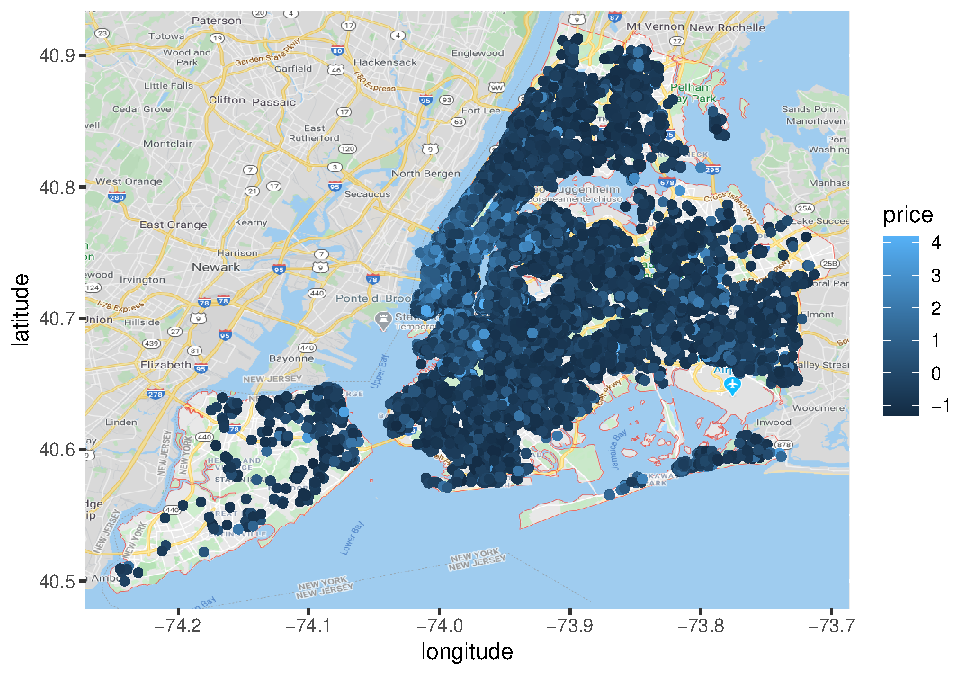
\includegraphics{project-code_files/figure-latex/unnamed-chunk-9-1.pdf}
~\\

\hypertarget{data-split}{%
\section{Data split}\label{data-split}}

\hypertarget{split-data-in-subsets-for-each-neighbourhood_group-and-room_type}{%
\subsection{Split data in subsets for each neighbourhood\_group and
room\_type}\label{split-data-in-subsets-for-each-neighbourhood_group-and-room_type}}

\begin{Shaded}
\begin{Highlighting}[]
\NormalTok{neighbourhoods =}\StringTok{ }\KeywordTok{unique}\NormalTok{(dataset}\OperatorTok{$}\NormalTok{neighbourhood_group)}

\NormalTok{rooms =}\StringTok{ }\KeywordTok{unique}\NormalTok{(dataset}\OperatorTok{$}\NormalTok{room_type)}

\NormalTok{clust_data =}\StringTok{ }\KeywordTok{vector}\NormalTok{(}\StringTok{"list"}\NormalTok{)}

\NormalTok{lis_n =}\StringTok{ }\KeywordTok{vector}\NormalTok{(}\StringTok{"list"}\NormalTok{)}

\ControlFlowTok{for}\NormalTok{ (n }\ControlFlowTok{in}\NormalTok{ neighbourhoods)}
\NormalTok{\{}
\NormalTok{  tmp =}\StringTok{ }\NormalTok{dataset }\OperatorTok\KeywordTok{filter}\NormalTok{( neighbourhood_group }\OperatorTok{==}\StringTok{ }\NormalTok{n) }
\NormalTok{  lis_n[[n]] =}\StringTok{ }\NormalTok{tmp[}\OperatorTok{-}\DecValTok{1}\NormalTok{]}
  
\NormalTok{  tmp2 =}\StringTok{ }\NormalTok{data }\OperatorTok\KeywordTok{filter}\NormalTok{( neighbourhood_group }\OperatorTok{==}\StringTok{ }\NormalTok{n) }
\NormalTok{  clust_data[[n]] =}\StringTok{ }\NormalTok{tmp2[}\OperatorTok{-}\DecValTok{1}\NormalTok{]}
\NormalTok{  clust_data[[n]]}\OperatorTok{$}\NormalTok{room_type =}\StringTok{ }\KeywordTok{factor}\NormalTok{(clust_data[[n]]}\OperatorTok{$}\NormalTok{room_type , }\DataTypeTok{level =} \KeywordTok{unique}\NormalTok{(clust_data[[n]]}\OperatorTok{$}\NormalTok{room_type) , }\DataTypeTok{labels=} \KeywordTok{unique}\NormalTok{(ds}\OperatorTok{$}\NormalTok{room_type))}
\NormalTok{\}}



\NormalTok{lis_r_n=}\StringTok{ }\KeywordTok{vector}\NormalTok{(}\StringTok{"list"}\NormalTok{)}
\ControlFlowTok{for}\NormalTok{ (n }\ControlFlowTok{in}\NormalTok{ neighbourhoods)}
\NormalTok{\{}
  \ControlFlowTok{for}\NormalTok{(r }\ControlFlowTok{in}\NormalTok{ rooms)}
\NormalTok{  \{}
\NormalTok{    tmp =}\StringTok{ }\NormalTok{dataset }\OperatorTok
\StringTok{      }\KeywordTok{filter}\NormalTok{( room_type }\OperatorTok{==}\StringTok{ }\NormalTok{r  }\OperatorTok{&}\StringTok{ }\NormalTok{neighbourhood_group }\OperatorTok{==}\StringTok{ }\NormalTok{n) }
\NormalTok{    lis_r_n[[}\KeywordTok{paste0}\NormalTok{(}\StringTok{"n"}\NormalTok{,n,}\StringTok{"-"}\NormalTok{,}\StringTok{"r"}\NormalTok{,r)]]=}\StringTok{ }\NormalTok{tmp[}\OperatorTok{-}\DecValTok{1}\NormalTok{][}\OperatorTok{-}\DecValTok{3}\NormalTok{]}
    
    
\NormalTok{    tmp2 =}\StringTok{ }\NormalTok{data }\OperatorTok
\StringTok{      }\KeywordTok{filter}\NormalTok{( room_type }\OperatorTok{==}\StringTok{ }\NormalTok{r  }\OperatorTok{&}\StringTok{ }\NormalTok{neighbourhood_group }\OperatorTok{==}\StringTok{ }\NormalTok{n) }
\NormalTok{    clust_data[[}\KeywordTok{paste0}\NormalTok{(}\StringTok{"n"}\NormalTok{,n,}\StringTok{"-"}\NormalTok{,}\StringTok{"r"}\NormalTok{,r)]]=}\StringTok{ }\NormalTok{tmp2[}\OperatorTok{-}\DecValTok{1}\NormalTok{][}\OperatorTok{-}\DecValTok{3}\NormalTok{]}
    
\NormalTok{  \}}
\NormalTok{\}}


\NormalTok{data}\OperatorTok{$}\NormalTok{neighbourhood_group =}\StringTok{ }\KeywordTok{factor}\NormalTok{(data}\OperatorTok{$}\NormalTok{neighbourhood_group  , }\DataTypeTok{level =} \KeywordTok{unique}\NormalTok{(data}\OperatorTok{$}\NormalTok{neighbourhood_group ) , }\DataTypeTok{labels=} \KeywordTok{unique}\NormalTok{(ds}\OperatorTok{$}\NormalTok{neighbourhood_group)) }
\NormalTok{data}\OperatorTok{$}\NormalTok{room_type =}\StringTok{ }\KeywordTok{factor}\NormalTok{(data}\OperatorTok{$}\NormalTok{room_type  , }\DataTypeTok{level =} \KeywordTok{unique}\NormalTok{(data}\OperatorTok{$}\NormalTok{room_type ) , }\DataTypeTok{labels=} \KeywordTok{unique}\NormalTok{(ds}\OperatorTok{$}\NormalTok{room_type)) }

\NormalTok{clust_data[[}\StringTok{"all"}\NormalTok{]] =}\StringTok{ }\NormalTok{data}
\end{Highlighting}
\end{Shaded}

~\\

\hypertarget{split-in-train-and-test-for-each-subset}{%
\subsection{Split in train and test for each
subset}\label{split-in-train-and-test-for-each-subset}}

\begin{Shaded}
\begin{Highlighting}[]
\NormalTok{trains =}\StringTok{ }\KeywordTok{vector}\NormalTok{(}\StringTok{"list"}\NormalTok{)}
\NormalTok{tests =}\StringTok{ }\KeywordTok{vector}\NormalTok{(}\StringTok{"list"}\NormalTok{)}
\NormalTok{datas =}\StringTok{ }\KeywordTok{vector}\NormalTok{(}\StringTok{"list"}\NormalTok{)}

\ControlFlowTok{for}\NormalTok{ (i }\ControlFlowTok{in} \KeywordTok{names}\NormalTok{(lis_n))}
\NormalTok{\{}
\NormalTok{  sample =}\StringTok{ }\KeywordTok{sample.split}\NormalTok{(lis_n[[i]], }\DataTypeTok{SplitRatio =} \FloatTok{.75}\NormalTok{)}
\NormalTok{  train =}\StringTok{ }\KeywordTok{subset}\NormalTok{(lis_n[[i]], sample }\OperatorTok{==}\StringTok{ }\OtherTok{TRUE}\NormalTok{)}
\NormalTok{  test  =}\StringTok{ }\KeywordTok{subset}\NormalTok{(lis_n[[i]], sample }\OperatorTok{==}\StringTok{ }\OtherTok{FALSE}\NormalTok{)}
\NormalTok{  trains[[i]]=}\StringTok{  }\NormalTok{train}
\NormalTok{  tests[[i]] =}\StringTok{ }\NormalTok{test}
\NormalTok{  datas[[i]] =}\StringTok{ }\NormalTok{lis_n[[i]]}
\NormalTok{\}}

\ControlFlowTok{for}\NormalTok{ (i }\ControlFlowTok{in} \KeywordTok{names}\NormalTok{(lis_r_n))}
\NormalTok{\{}
\NormalTok{  sample =}\StringTok{ }\KeywordTok{sample.split}\NormalTok{(lis_r_n[[i]], }\DataTypeTok{SplitRatio =} \FloatTok{.75}\NormalTok{)}
\NormalTok{  train =}\StringTok{ }\KeywordTok{subset}\NormalTok{(lis_r_n[[i]], sample }\OperatorTok{==}\StringTok{ }\OtherTok{TRUE}\NormalTok{)}
\NormalTok{  test  =}\StringTok{ }\KeywordTok{subset}\NormalTok{(lis_r_n[[i]], sample }\OperatorTok{==}\StringTok{ }\OtherTok{FALSE}\NormalTok{)}
\NormalTok{  trains[[i]]=}\StringTok{  }\NormalTok{train}
\NormalTok{  tests[[i]] =}\StringTok{ }\NormalTok{test}
\NormalTok{  datas[[i]] =}\StringTok{ }\NormalTok{lis_r_n[[i]]}
  
\NormalTok{\}}

\NormalTok{sample =}\StringTok{ }\KeywordTok{sample.split}\NormalTok{(dataset, }\DataTypeTok{SplitRatio =} \FloatTok{.75}\NormalTok{)}
\NormalTok{train =}\StringTok{ }\KeywordTok{subset}\NormalTok{(dataset, sample }\OperatorTok{==}\StringTok{ }\OtherTok{TRUE}\NormalTok{)}
\NormalTok{test  =}\StringTok{ }\KeywordTok{subset}\NormalTok{(dataset, sample }\OperatorTok{==}\StringTok{ }\OtherTok{FALSE}\NormalTok{)}

\NormalTok{trains[[}\StringTok{"all"}\NormalTok{]] =}\StringTok{ }\NormalTok{train}
\NormalTok{tests[[}\StringTok{"all"}\NormalTok{]] =}\StringTok{ }\NormalTok{test}
\NormalTok{datas[[}\StringTok{"all"}\NormalTok{]] =}\StringTok{ }\NormalTok{dataset}
\end{Highlighting}
\end{Shaded}

~\\

\hypertarget{models-train}{%
\section{MODELS TRAIN}\label{models-train}}

~\\

\begin{Shaded}
\begin{Highlighting}[]
\NormalTok{model_lis =}\StringTok{ }\KeywordTok{vector}\NormalTok{(}\StringTok{"list"}\NormalTok{)}
\end{Highlighting}
\end{Shaded}

~\\

\hypertarget{linear-regression}{%
\subsection{LINEAR REGRESSION}\label{linear-regression}}

\begin{Shaded}
\begin{Highlighting}[]
\NormalTok{lin_reg =}\StringTok{ }\KeywordTok{vector}\NormalTok{(}\StringTok{"list"}\NormalTok{)}

\ControlFlowTok{for}\NormalTok{ (sub }\ControlFlowTok{in} \KeywordTok{names}\NormalTok{(trains))}
\NormalTok{\{}
\NormalTok{  lin_reg[[sub]]}\OperatorTok{$}\NormalTok{fit =lm.fit =}\StringTok{ }\KeywordTok{lm}\NormalTok{(price}\OperatorTok{~}\NormalTok{., }\DataTypeTok{data =}\NormalTok{ trains[[sub]])}
\NormalTok{  lin_reg[[sub]]}\OperatorTok{$}\NormalTok{summary =}\StringTok{ }\KeywordTok{summary}\NormalTok{(lm.fit)}
  
\NormalTok{  lin_reg[[sub]]}\OperatorTok{$}\NormalTok{pred  =}\StringTok{ }\NormalTok{pr.lm =}\StringTok{ }\KeywordTok{predict}\NormalTok{(lm.fit,tests[[sub]])}
  
\NormalTok{  lin_reg[[sub]]}\OperatorTok{$}\NormalTok{MSE =}\StringTok{ }\KeywordTok{sum}\NormalTok{((pr.lm }\OperatorTok{-}\StringTok{ }\NormalTok{tests[[sub]]}\OperatorTok{$}\NormalTok{price)}\OperatorTok{^}\DecValTok{2}\NormalTok{)}\OperatorTok{/}\KeywordTok{nrow}\NormalTok{(tests[[sub]])}
  \KeywordTok{print}\NormalTok{(}\KeywordTok{paste0}\NormalTok{(}\StringTok{"========== "}\NormalTok{,sub, }\StringTok{" =========="}\NormalTok{))}
  \KeywordTok{print}\NormalTok{(}\KeywordTok{summary}\NormalTok{(lm.fit))}
  \KeywordTok{cat}\NormalTok{(}\StringTok{"}\CharTok{\textbackslash{}n\textbackslash{}n}\StringTok{"}\NormalTok{)}
\NormalTok{\}}
\end{Highlighting}
\end{Shaded}

\begin{verbatim}
## [1] "========== 1 =========="
## 
## Call:
## lm(formula = price ~ ., data = trains[[sub]])
## 
## Residuals:
##     Min      1Q  Median      3Q     Max 
## -1.8323 -0.3481 -0.1192  0.1750  5.3768 
## 
## Coefficients:
##               Estimate Std. Error t value Pr(>|t|)    
## (Intercept) -573.61243   20.31625 -28.234  < 2e-16 ***
## latitude       5.38922    0.20629  26.124  < 2e-16 ***
## longitude     -4.78267    0.22513 -21.244  < 2e-16 ***
## room_type2     0.96362    0.01128  85.441  < 2e-16 ***
## room_type3    -0.18322    0.03931  -4.661 3.17e-06 ***
## ---
## Signif. codes:  0 '***' 0.001 '**' 0.01 '*' 0.05 '.' 0.1 ' ' 1
## 
## Residual standard error: 0.6717 on 14888 degrees of freedom
## Multiple R-squared:  0.3869, Adjusted R-squared:  0.3867 
## F-statistic:  2348 on 4 and 14888 DF,  p-value: < 2.2e-16
## 
## 
## 
## [1] "========== 2 =========="
## 
## Call:
## lm(formula = price ~ ., data = trains[[sub]])
## 
## Residuals:
##     Min      1Q  Median      3Q     Max 
## -2.4058 -0.5348 -0.1896  0.2846  4.7774 
## 
## Coefficients:
##               Estimate Std. Error t value Pr(>|t|)    
## (Intercept) -845.59998   58.81126 -14.378  < 2e-16 ***
## latitude      -0.46594    0.35605  -1.309    0.191    
## longitude    -11.68449    0.62124 -18.808  < 2e-16 ***
## room_type2     1.01872    0.01503  67.766  < 2e-16 ***
## room_type3    -0.26290    0.04863  -5.406 6.52e-08 ***
## ---
## Signif. codes:  0 '***' 0.001 '**' 0.01 '*' 0.05 '.' 0.1 ' ' 1
## 
## Residual standard error: 0.8837 on 15653 degrees of freedom
## Multiple R-squared:  0.3343, Adjusted R-squared:  0.3341 
## F-statistic:  1965 on 4 and 15653 DF,  p-value: < 2.2e-16
## 
## 
## 
## [1] "========== 3 =========="
## 
## Call:
## lm(formula = price ~ ., data = trains[[sub]])
## 
## Residuals:
##     Min      1Q  Median      3Q     Max 
## -1.3742 -0.2988 -0.1270  0.1391  5.0902 
## 
## Coefficients:
##             Estimate Std. Error t value Pr(>|t|)    
## (Intercept) -7.94589   12.53702  -0.634  0.52625    
## latitude    -0.67106    0.28710  -2.337  0.01947 *  
## longitude   -0.46762    0.20025  -2.335  0.01958 *  
## room_type2   0.80929    0.01951  41.478  < 2e-16 ***
## room_type3  -0.17440    0.05165  -3.377  0.00074 ***
## ---
## Signif. codes:  0 '***' 0.001 '**' 0.01 '*' 0.05 '.' 0.1 ' ' 1
## 
## Residual standard error: 0.6028 on 4219 degrees of freedom
## Multiple R-squared:  0.3044, Adjusted R-squared:  0.3037 
## F-statistic: 461.5 on 4 and 4219 DF,  p-value: < 2.2e-16
## 
## 
## 
## [1] "========== 4 =========="
## 
## Call:
## lm(formula = price ~ ., data = trains[[sub]])
## 
## Residuals:
##     Min      1Q  Median      3Q     Max 
## -0.9120 -0.3348 -0.1459  0.2172  3.6564 
## 
## Coefficients:
##               Estimate Std. Error t value Pr(>|t|)    
## (Intercept) -30.688887 144.852858  -0.212    0.832    
## latitude      0.734021   1.511517   0.486    0.628    
## longitude    -0.001178   1.331628  -0.001    0.999    
## room_type2    0.739498   0.078599   9.408   <2e-16 ***
## room_type3    0.159594   0.292213   0.546    0.585    
## ---
## Signif. codes:  0 '***' 0.001 '**' 0.01 '*' 0.05 '.' 0.1 ' ' 1
## 
## Residual standard error: 0.6387 on 269 degrees of freedom
## Multiple R-squared:  0.2493, Adjusted R-squared:  0.2382 
## F-statistic: 22.34 on 4 and 269 DF,  p-value: 6.126e-16
## 
## 
## 
## [1] "========== 5 =========="
## 
## Call:
## lm(formula = price ~ ., data = trains[[sub]])
## 
## Residuals:
##     Min      1Q  Median      3Q     Max 
## -0.9669 -0.2906 -0.1359  0.1124  4.9772 
## 
## Coefficients:
##             Estimate Std. Error t value Pr(>|t|)    
## (Intercept) 62.09595   75.12511   0.827    0.409    
## latitude    -0.46076    0.89539  -0.515    0.607    
## longitude    0.59638    0.72879   0.818    0.413    
## room_type2   0.67380    0.04732  14.238   <2e-16 ***
## room_type3  -0.15156    0.09529  -1.591    0.112    
## ---
## Signif. codes:  0 '***' 0.001 '**' 0.01 '*' 0.05 '.' 0.1 ' ' 1
## 
## Residual standard error: 0.6266 on 806 degrees of freedom
## Multiple R-squared:  0.2199, Adjusted R-squared:  0.216 
## F-statistic: 56.79 on 4 and 806 DF,  p-value: < 2.2e-16
## 
## 
## 
## [1] "========== n1-r1 =========="
## 
## Call:
## lm(formula = price ~ ., data = trains[[sub]])
## 
## Residuals:
##     Min      1Q  Median      3Q     Max 
## -0.7175 -0.2367 -0.0890  0.1093  5.1328 
## 
## Coefficients:
##              Estimate Std. Error t value Pr(>|t|)    
## (Intercept) -351.5686    19.4645  -18.06   <2e-16 ***
## latitude       2.8562     0.1986   14.38   <2e-16 ***
## longitude     -3.1736     0.2130  -14.90   <2e-16 ***
## ---
## Signif. codes:  0 '***' 0.001 '**' 0.01 '*' 0.05 '.' 0.1 ' ' 1
## 
## Residual standard error: 0.4244 on 6721 degrees of freedom
## Multiple R-squared:  0.0483, Adjusted R-squared:  0.04802 
## F-statistic: 170.6 on 2 and 6721 DF,  p-value: < 2.2e-16
## 
## 
## 
## [1] "========== n1-r2 =========="
## 
## Call:
## lm(formula = price ~ ., data = trains[[sub]])
## 
## Residuals:
##     Min      1Q  Median      3Q     Max 
## -1.9631 -0.5724 -0.2106  0.2963  4.4458 
## 
## Coefficients:
##              Estimate Std. Error t value Pr(>|t|)    
## (Intercept) -764.9500    39.6271  -19.30   <2e-16 ***
## latitude       8.2186     0.4068   20.20   <2e-16 ***
## longitude     -5.8264     0.4454  -13.08   <2e-16 ***
## ---
## Signif. codes:  0 '***' 0.001 '**' 0.01 '*' 0.05 '.' 0.1 ' ' 1
## 
## Residual standard error: 0.8599 on 6238 degrees of freedom
## Multiple R-squared:  0.07359,    Adjusted R-squared:  0.07329 
## F-statistic: 247.7 on 2 and 6238 DF,  p-value: < 2.2e-16
## 
## 
## 
## [1] "========== n1-r3 =========="
## 
## Call:
## lm(formula = price ~ ., data = trains[[sub]])
## 
## Residuals:
##      Min       1Q   Median       3Q      Max 
## -0.43709 -0.22328 -0.13609  0.05886  2.72639 
## 
## Coefficients:
##              Estimate Std. Error t value Pr(>|t|)    
## (Intercept) -322.3727    94.7421  -3.403 0.000769 ***
## latitude       2.8413     0.7927   3.584 0.000401 ***
## longitude     -2.7841     1.0335  -2.694 0.007504 ** 
## ---
## Signif. codes:  0 '***' 0.001 '**' 0.01 '*' 0.05 '.' 0.1 ' ' 1
## 
## Residual standard error: 0.4409 on 270 degrees of freedom
## Multiple R-squared:  0.05102,    Adjusted R-squared:  0.04399 
## F-statistic: 7.258 on 2 and 270 DF,  p-value: 0.0008505
## 
## 
## 
## [1] "========== n2-r1 =========="
## 
## Call:
## lm(formula = price ~ ., data = trains[[sub]])
## 
## Residuals:
##     Min      1Q  Median      3Q     Max 
## -1.2007 -0.3766 -0.1682  0.1281  4.7297 
## 
## Coefficients:
##              Estimate Std. Error t value Pr(>|t|)    
## (Intercept) -673.3536    81.3847  -8.274   <2e-16 ***
## latitude      -0.5113     0.4675  -1.094    0.274    
## longitude     -9.3809     0.8670 -10.820   <2e-16 ***
## ---
## Signif. codes:  0 '***' 0.001 '**' 0.01 '*' 0.05 '.' 0.1 ' ' 1
## 
## Residual standard error: 0.6845 on 5252 degrees of freedom
## Multiple R-squared:  0.1039, Adjusted R-squared:  0.1036 
## F-statistic: 304.5 on 2 and 5252 DF,  p-value: < 2.2e-16
## 
## 
## 
## [1] "========== n2-r2 =========="
## 
## Call:
## lm(formula = price ~ ., data = trains[[sub]])
## 
## Residuals:
##     Min      1Q  Median      3Q     Max 
## -2.4464 -0.6834 -0.2428  0.4327  3.8755 
## 
## Coefficients:
##              Estimate Std. Error t value Pr(>|t|)    
## (Intercept) -888.5411    89.7697  -9.898   <2e-16 ***
## latitude      -0.9338     0.5683  -1.643      0.1    
## longitude    -12.5366     0.9398 -13.339   <2e-16 ***
## ---
## Signif. codes:  0 '***' 0.001 '**' 0.01 '*' 0.05 '.' 0.1 ' ' 1
## 
## Residual standard error: 0.9986 on 8343 degrees of freedom
## Multiple R-squared:  0.07902,    Adjusted R-squared:  0.0788 
## F-statistic: 357.9 on 2 and 8343 DF,  p-value: < 2.2e-16
## 
## 
## 
## [1] "========== n2-r3 =========="
## 
## Call:
## lm(formula = price ~ ., data = trains[[sub]])
## 
## Residuals:
##     Min      1Q  Median      3Q     Max 
## -0.8824 -0.3980 -0.2476  0.0510  4.5630 
## 
## Coefficients:
##              Estimate Std. Error t value Pr(>|t|)    
## (Intercept) -1089.024    345.497  -3.152 0.001778 ** 
## latitude        3.921      2.098   1.869 0.062580 .  
## longitude     -12.554      3.676  -3.415 0.000723 ***
## ---
## Signif. codes:  0 '***' 0.001 '**' 0.01 '*' 0.05 '.' 0.1 ' ' 1
## 
## Residual standard error: 0.7959 on 313 degrees of freedom
## Multiple R-squared:  0.04358,    Adjusted R-squared:  0.03747 
## F-statistic: 7.132 on 2 and 313 DF,  p-value: 0.0009361
## 
## 
## 
## [1] "========== n3-r1 =========="
## 
## Call:
## lm(formula = price ~ ., data = trains[[sub]])
## 
## Residuals:
##     Min      1Q  Median      3Q     Max 
## -0.5259 -0.2303 -0.0979  0.1135  4.6236 
## 
## Coefficients:
##             Estimate Std. Error t value Pr(>|t|)  
## (Intercept) -18.6830    12.6014  -1.483   0.1383  
## latitude     -0.2314     0.2962  -0.781   0.4346  
## longitude    -0.3707     0.1963  -1.888   0.0591 .
## ---
## Signif. codes:  0 '***' 0.001 '**' 0.01 '*' 0.05 '.' 0.1 ' ' 1
## 
## Residual standard error: 0.4295 on 2239 degrees of freedom
## Multiple R-squared:  0.001641,   Adjusted R-squared:  0.0007496 
## F-statistic: 1.841 on 2 and 2239 DF,  p-value: 0.159
## 
## 
## 
## [1] "========== n3-r2 =========="
## 
## Call:
## lm(formula = price ~ ., data = trains[[sub]])
## 
## Residuals:
##     Min      1Q  Median      3Q     Max 
## -1.3548 -0.5229 -0.2095  0.2175  4.1989 
## 
## Coefficients:
##             Estimate Std. Error t value Pr(>|t|)  
## (Intercept) -14.6167    28.3789  -0.515   0.6066  
## latitude     -1.2073     0.6411  -1.883   0.0599 .
## longitude    -0.8644     0.4822  -1.793   0.0732 .
## ---
## Signif. codes:  0 '***' 0.001 '**' 0.01 '*' 0.05 '.' 0.1 ' ' 1
## 
## Residual standard error: 0.8256 on 1381 degrees of freedom
## Multiple R-squared:  0.003026,   Adjusted R-squared:  0.001582 
## F-statistic: 2.096 on 2 and 1381 DF,  p-value: 0.1233
## 
## 
## 
## [1] "========== n3-r3 =========="
## 
## Call:
## lm(formula = price ~ ., data = trains[[sub]])
## 
## Residuals:
##     Min      1Q  Median      3Q     Max 
## -0.4426 -0.2340 -0.1254  0.0081  5.0332 
## 
## Coefficients:
##              Estimate Std. Error t value Pr(>|t|)
## (Intercept) -113.4214    81.6764  -1.389    0.167
## latitude       2.9879     2.0923   1.428    0.156
## longitude      0.1248     1.2873   0.097    0.923
## 
## Residual standard error: 0.5843 on 126 degrees of freedom
## Multiple R-squared:  0.0226, Adjusted R-squared:  0.007089 
## F-statistic: 1.457 on 2 and 126 DF,  p-value: 0.2368
## 
## 
## 
## [1] "========== n4-r1 =========="
## 
## Call:
## lm(formula = price ~ ., data = trains[[sub]])
## 
## Residuals:
##     Min      1Q  Median      3Q     Max 
## -0.4399 -0.2616 -0.1008  0.1382  2.7047 
## 
## Coefficients:
##             Estimate Std. Error t value Pr(>|t|)
## (Intercept)  41.8452   140.4584   0.298    0.766
## latitude     -1.3294     1.5633  -0.850    0.397
## longitude    -0.1532     1.3589  -0.113    0.910
## 
## Residual standard error: 0.4341 on 123 degrees of freedom
## Multiple R-squared:  0.008143,   Adjusted R-squared:  -0.007985 
## F-statistic: 0.5049 on 2 and 123 DF,  p-value: 0.6048
## 
## 
## 
## [1] "========== n4-r2 =========="
## 
## Call:
## lm(formula = price ~ ., data = trains[[sub]])
## 
## Residuals:
##     Min      1Q  Median      3Q     Max 
## -0.9076 -0.5490 -0.2720  0.2208  3.6389 
## 
## Coefficients:
##             Estimate Std. Error t value Pr(>|t|)
## (Intercept)   40.350    296.277   0.136    0.892
## latitude       1.207      2.991   0.403    0.687
## longitude      1.207      2.710   0.445    0.657
## 
## Residual standard error: 0.8287 on 110 degrees of freedom
## Multiple R-squared:  0.009854,   Adjusted R-squared:  -0.008149 
## F-statistic: 0.5474 on 2 and 110 DF,  p-value: 0.58
## 
## 
## 
## [1] "========== n4-r3 =========="
## 
## Call:
## lm(formula = price ~ ., data = trains[[sub]])
## 
## Residuals:
##        1        3        4        6        7 
##  0.05210  0.05313  0.06896  0.03662 -0.21082 
## 
## Coefficients:
##              Estimate Std. Error t value Pr(>|t|)
## (Intercept) -1780.567   3072.654  -0.579    0.621
## latitude       26.744     13.141   2.035    0.179
## longitude      -9.363     35.224  -0.266    0.815
## 
## Residual standard error: 0.1675 on 2 degrees of freedom
## Multiple R-squared:  0.8503, Adjusted R-squared:  0.7006 
## F-statistic:  5.68 on 2 and 2 DF,  p-value: 0.1497
## 
## 
## 
## [1] "========== n5-r1 =========="
## 
## Call:
## lm(formula = price ~ ., data = trains[[sub]])
## 
## Residuals:
##     Min      1Q  Median      3Q     Max 
## -0.4612 -0.2341 -0.0916  0.1272  4.9178 
## 
## Coefficients:
##             Estimate Std. Error t value Pr(>|t|)  
## (Intercept)  88.3541    73.8984   1.196   0.2325  
## latitude     -1.9505     0.8424  -2.315   0.0211 *
## longitude     0.1284     0.7459   0.172   0.8634  
## ---
## Signif. codes:  0 '***' 0.001 '**' 0.01 '*' 0.05 '.' 0.1 ' ' 1
## 
## Residual standard error: 0.4251 on 429 degrees of freedom
## Multiple R-squared:  0.01321,    Adjusted R-squared:  0.00861 
## F-statistic: 2.872 on 2 and 429 DF,  p-value: 0.05769
## 
## 
## 
## [1] "========== n5-r2 =========="
## 
## Call:
## lm(formula = price ~ ., data = trains[[sub]])
## 
## Residuals:
##     Min      1Q  Median      3Q     Max 
## -1.1899 -0.4834 -0.2201  0.1913  4.2329 
## 
## Coefficients:
##               Estimate Std. Error t value Pr(>|t|)
## (Intercept) -100.40099  164.61869  -0.610    0.542
## latitude       2.57087    2.05784   1.249    0.213
## longitude      0.06421    1.54657   0.042    0.967
## 
## Residual standard error: 0.8279 on 248 degrees of freedom
## Multiple R-squared:  0.007378,   Adjusted R-squared:  -0.0006266 
## F-statistic: 0.9217 on 2 and 248 DF,  p-value: 0.3992
## 
## 
## 
## [1] "========== n5-r3 =========="
## 
## Call:
## lm(formula = price ~ ., data = trains[[sub]])
## 
## Residuals:
##      Min       1Q   Median       3Q      Max 
## -0.40836 -0.14435 -0.05595  0.06429  1.04848 
## 
## Coefficients:
##             Estimate Std. Error t value Pr(>|t|)
## (Intercept)   77.152    186.703   0.413    0.682
## latitude       1.712      2.084   0.822    0.417
## longitude      2.004      1.707   1.174    0.248
## 
## Residual standard error: 0.2919 on 36 degrees of freedom
## Multiple R-squared:  0.1093, Adjusted R-squared:  0.05986 
## F-statistic:  2.21 on 2 and 36 DF,  p-value: 0.1244
## 
## 
## 
## [1] "========== all =========="
## 
## Call:
## lm(formula = price ~ ., data = trains[[sub]])
## 
## Residuals:
##     Min      1Q  Median      3Q     Max 
## -2.2177 -0.4433 -0.1399  0.2223  5.0722 
## 
## Coefficients:
##                        Estimate Std. Error t value Pr(>|t|)    
## (Intercept)          -2.038e+02  1.411e+01 -14.446  < 2e-16 ***
## neighbourhood_group2  4.855e-01  1.608e-02  30.189  < 2e-16 ***
## neighbourhood_group3  2.352e-01  1.963e-02  11.979  < 2e-16 ***
## neighbourhood_group4 -8.552e-01  5.697e-02 -15.012  < 2e-16 ***
## neighbourhood_group5  2.821e-01  3.838e-02   7.350 2.04e-13 ***
## latitude             -1.413e+00  1.382e-01 -10.227  < 2e-16 ***
## longitude            -3.524e+00  1.587e-01 -22.204  < 2e-16 ***
## room_type2            9.844e-01  9.582e-03 102.736  < 2e-16 ***
## room_type3           -2.466e-01  3.070e-02  -8.032 9.94e-16 ***
## ---
## Signif. codes:  0 '***' 0.001 '**' 0.01 '*' 0.05 '.' 0.1 ' ' 1
## 
## Residual standard error: 0.7784 on 28680 degrees of freedom
## Multiple R-squared:  0.3889, Adjusted R-squared:  0.3888 
## F-statistic:  2282 on 8 and 28680 DF,  p-value: < 2.2e-16
\end{verbatim}

\begin{Shaded}
\begin{Highlighting}[]
\NormalTok{lin_reg}\OperatorTok{$}\NormalTok{name =}\StringTok{ "Linear Regression"}
\NormalTok{model_lis}\OperatorTok{$}\NormalTok{linear_regression=}\StringTok{  }\NormalTok{lin_reg}
\end{Highlighting}
\end{Shaded}

~\\

\hypertarget{decision-tree}{%
\subsection{DECISION TREE}\label{decision-tree}}

\begin{Shaded}
\begin{Highlighting}[]
\NormalTok{dec_tree =}\StringTok{ }\KeywordTok{vector}\NormalTok{(}\StringTok{"list"}\NormalTok{)}

\ControlFlowTok{for}\NormalTok{ (sub }\ControlFlowTok{in} \KeywordTok{names}\NormalTok{(trains))}
\NormalTok{\{}
\NormalTok{  dec_tree[[sub]]}\OperatorTok{$}\NormalTok{fit =}\StringTok{ }\NormalTok{tree_res=}\KeywordTok{tree}\NormalTok{(price}\OperatorTok{~}\NormalTok{., }\DataTypeTok{data =}\NormalTok{ trains[[sub]])}
\NormalTok{  dec_tree[[sub]]}\OperatorTok{$}\NormalTok{summary =}\StringTok{ }\NormalTok{sum =}\StringTok{ }\KeywordTok{summary}\NormalTok{(tree_res)}
  
  \KeywordTok{print}\NormalTok{(}\KeywordTok{paste0}\NormalTok{(}\StringTok{"========== "}\NormalTok{,sub, }\StringTok{" =========="}\NormalTok{))}

  \KeywordTok{print}\NormalTok{(sum)}
  
  \ControlFlowTok{if}\NormalTok{(sum}\OperatorTok{$}\NormalTok{size }\OperatorTok{>}\StringTok{ }\DecValTok{1}\NormalTok{ )}
\NormalTok{  \{}
    \KeywordTok{plot}\NormalTok{(tree_res)}
    \KeywordTok{text}\NormalTok{(tree_res,}\DataTypeTok{pretty=}\DecValTok{0}\NormalTok{)}
    \KeywordTok{title}\NormalTok{(}\KeywordTok{paste0}\NormalTok{(}\StringTok{"Tree of: "}\NormalTok{,sub))}
    
   
\NormalTok{  \}}
  \ControlFlowTok{else} 
\NormalTok{  \{}
    \KeywordTok{cat}\NormalTok{(}\StringTok{"Not possible to plot tree: "}\NormalTok{, sub)}
\NormalTok{  \}}
  
\NormalTok{  dec_tree[[sub]]}\OperatorTok{$}\NormalTok{pred  =}\StringTok{ }\NormalTok{pred =}\StringTok{ }\KeywordTok{predict}\NormalTok{(tree_res,tests[[sub]])}
  
\NormalTok{  dec_tree[[sub]]}\OperatorTok{$}\NormalTok{MSE =}\StringTok{ }\NormalTok{mse =}\StringTok{  }\KeywordTok{sum}\NormalTok{((pred }\OperatorTok{-}\StringTok{ }\NormalTok{tests[[sub]]}\OperatorTok{$}\NormalTok{price)}\OperatorTok{^}\DecValTok{2}\NormalTok{)}\OperatorTok{/}\KeywordTok{nrow}\NormalTok{(tests[[sub]])}
  \KeywordTok{print}\NormalTok{(mse)}
  \KeywordTok{cat}\NormalTok{(}\StringTok{"}\CharTok{\textbackslash{}n\textbackslash{}n}\StringTok{"}\NormalTok{)}
\NormalTok{\}}
\end{Highlighting}
\end{Shaded}

\begin{verbatim}
## [1] "========== 1 =========="
## 
## Regression tree:
## tree(formula = price ~ ., data = trains[[sub]])
## Number of terminal nodes:  5 
## Residual mean deviance:  0.4464 = 6645 / 14890 
## Distribution of residuals:
##    Min. 1st Qu.  Median    Mean 3rd Qu.    Max. 
## -1.9250 -0.3460 -0.1188  0.0000  0.1652  4.8800
\end{verbatim}

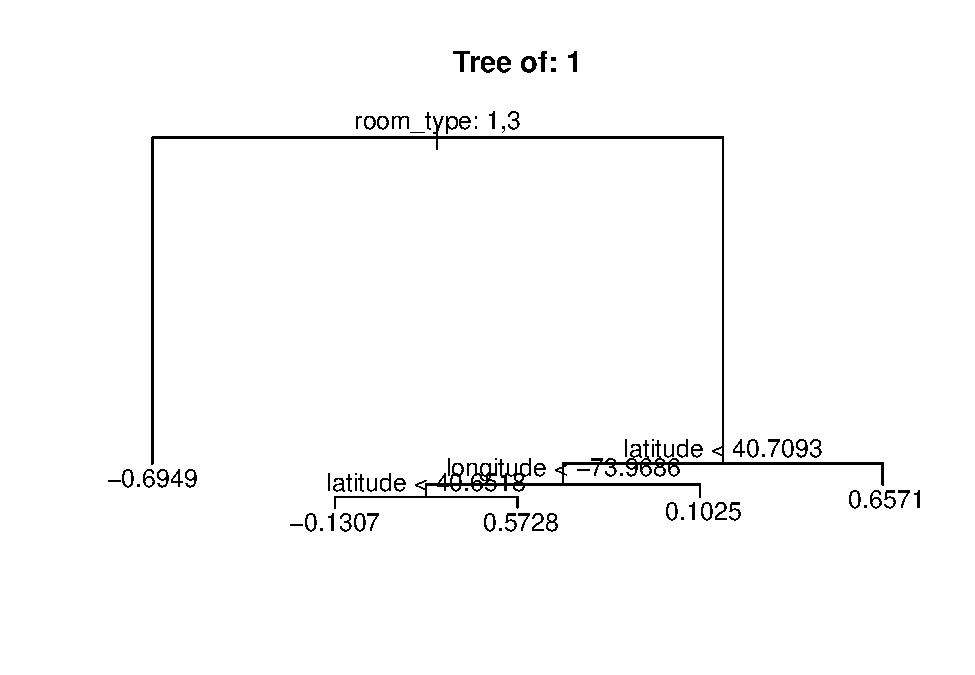
\includegraphics{project-code_files/figure-latex/unnamed-chunk-14-1.pdf}

\begin{verbatim}
## [1] 0.4607817
## 
## 
## [1] "========== 2 =========="
## 
## Regression tree:
## tree(formula = price ~ ., data = trains[[sub]])
## Variables actually used in tree construction:
## [1] "room_type" "longitude"
## Number of terminal nodes:  4 
## Residual mean deviance:  0.7869 = 12320 / 15650 
## Distribution of residuals:
##    Min. 1st Qu.  Median    Mean 3rd Qu.    Max. 
## -2.2850 -0.5200 -0.1947  0.0000  0.2965  4.7620
\end{verbatim}

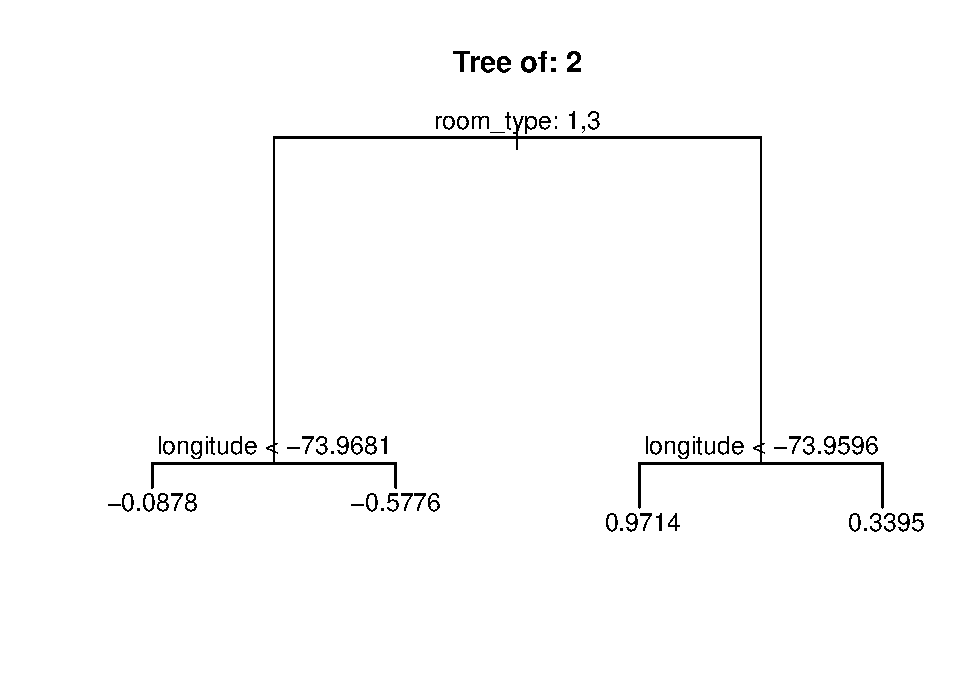
\includegraphics{project-code_files/figure-latex/unnamed-chunk-14-2.pdf}

\begin{verbatim}
## [1] 0.7634093
## 
## 
## [1] "========== 3 =========="
## 
## Regression tree:
## tree(formula = price ~ ., data = trains[[sub]])
## Variables actually used in tree construction:
## [1] "room_type"
## Number of terminal nodes:  2 
## Residual mean deviance:  0.3647 = 1540 / 4222 
## Distribution of residuals:
##    Min. 1st Qu.  Median    Mean 3rd Qu.    Max. 
## -1.3900 -0.3014 -0.1245  0.0000  0.1319  4.9310
\end{verbatim}

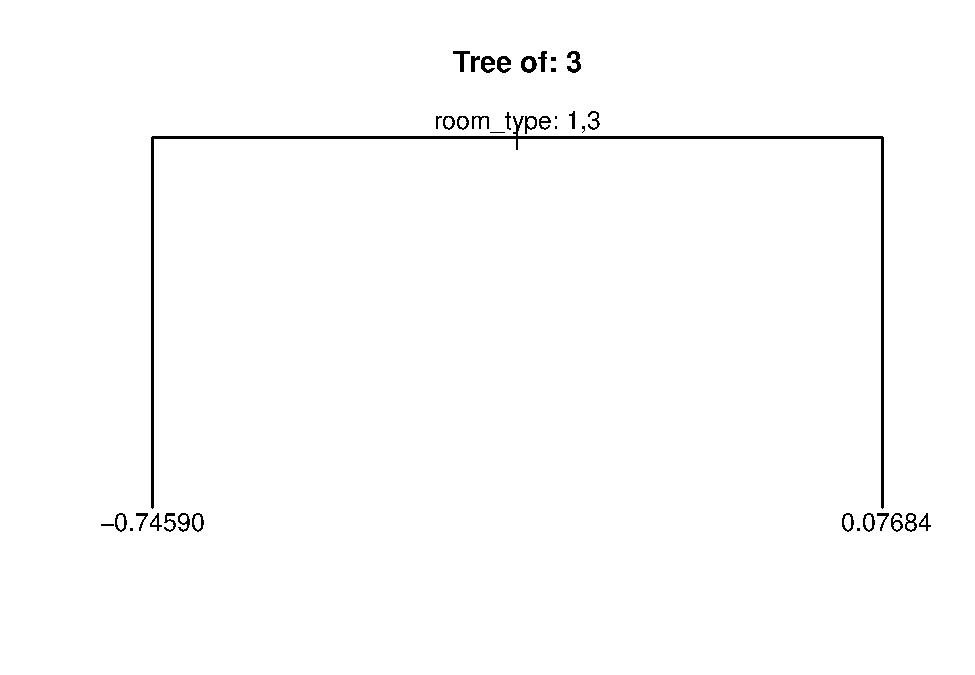
\includegraphics{project-code_files/figure-latex/unnamed-chunk-14-3.pdf}

\begin{verbatim}
## [1] 0.3864543
## 
## 
## [1] "========== 4 =========="
## 
## Regression tree:
## tree(formula = price ~ ., data = trains[[sub]])
## Number of terminal nodes:  10 
## Residual mean deviance:  0.3202 = 84.54 / 264 
## Distribution of residuals:
##    Min. 1st Qu.  Median    Mean 3rd Qu.    Max. 
## -1.3500 -0.3039 -0.1221  0.0000  0.2187  2.3540
\end{verbatim}

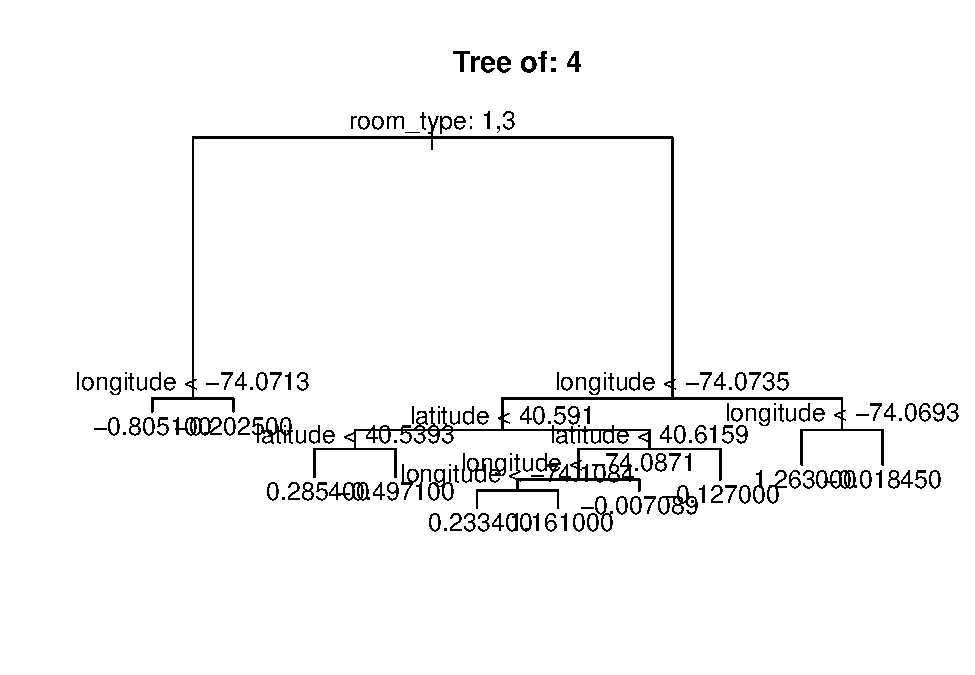
\includegraphics{project-code_files/figure-latex/unnamed-chunk-14-4.pdf}

\begin{verbatim}
## [1] 0.3471879
## 
## 
## [1] "========== 5 =========="
## 
## Regression tree:
## tree(formula = price ~ ., data = trains[[sub]])
## Variables actually used in tree construction:
## [1] "room_type"
## Number of terminal nodes:  2 
## Residual mean deviance:  0.3927 = 317.7 / 809 
## Distribution of residuals:
##    Min. 1st Qu.  Median    Mean 3rd Qu.    Max. 
## -0.9862 -0.2943 -0.1239  0.0000  0.1033  4.9880
\end{verbatim}

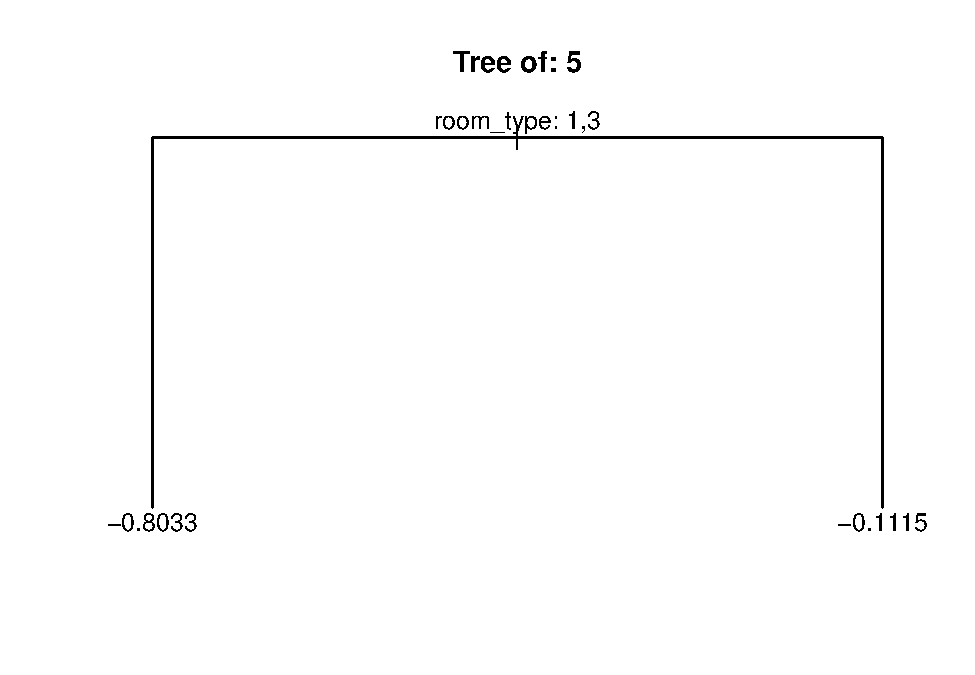
\includegraphics{project-code_files/figure-latex/unnamed-chunk-14-5.pdf}

\begin{verbatim}
## [1] 0.2744778
## 
## 
## [1] "========== n1-r1 =========="
## 
## Regression tree:
## tree(formula = price ~ ., data = trains[[sub]])
## Number of terminal nodes:  4 
## Residual mean deviance:  0.1738 = 1168 / 6720 
## Distribution of residuals:
##    Min. 1st Qu.  Median    Mean 3rd Qu.    Max. 
## -0.7561 -0.2242 -0.0745  0.0000  0.1166  4.9440
\end{verbatim}

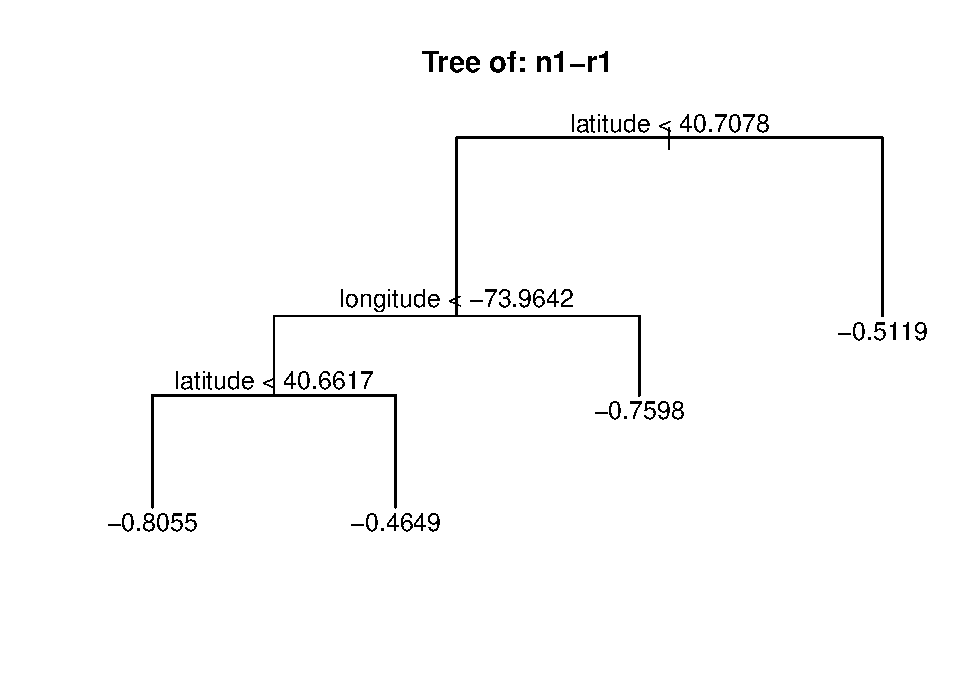
\includegraphics{project-code_files/figure-latex/unnamed-chunk-14-6.pdf}

\begin{verbatim}
## [1] 0.1771088
## 
## 
## [1] "========== n1-r2 =========="
## 
## Regression tree:
## tree(formula = price ~ ., data = trains[[sub]])
## Number of terminal nodes:  4 
## Residual mean deviance:  0.731 = 4559 / 6237 
## Distribution of residuals:
##    Min. 1st Qu.  Median    Mean 3rd Qu.    Max. 
## -1.9250 -0.5518 -0.2070  0.0000  0.3002  4.0740
\end{verbatim}

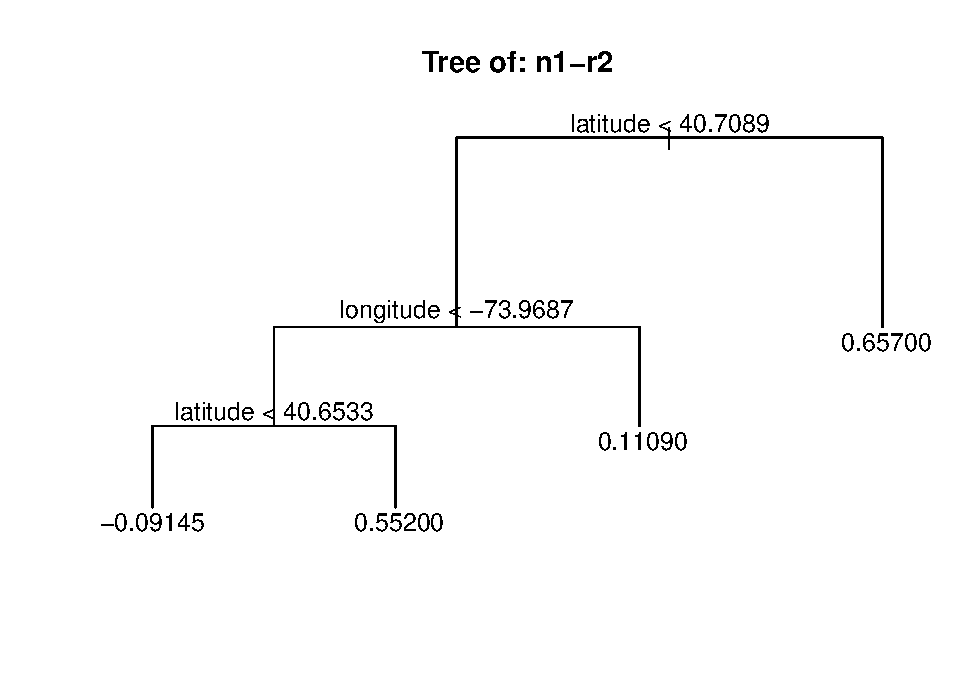
\includegraphics{project-code_files/figure-latex/unnamed-chunk-14-7.pdf}

\begin{verbatim}
## [1] 0.7503308
## 
## 
## [1] "========== n1-r3 =========="
## 
## Regression tree:
## tree(formula = price ~ ., data = trains[[sub]])
## Number of terminal nodes:  8 
## Residual mean deviance:  0.1442 = 38.21 / 265 
## Distribution of residuals:
##     Min.  1st Qu.   Median     Mean  3rd Qu.     Max. 
## -1.02700 -0.15190 -0.06911  0.00000  0.04448  2.05000
\end{verbatim}

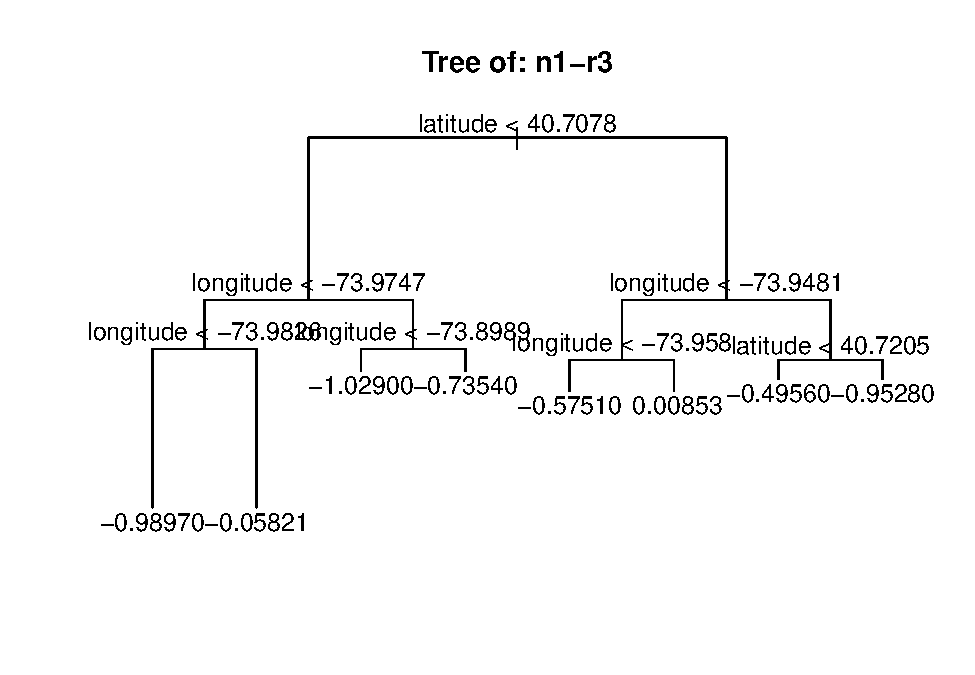
\includegraphics{project-code_files/figure-latex/unnamed-chunk-14-8.pdf}

\begin{verbatim}
## [1] 0.2505339
## 
## 
## [1] "========== n2-r1 =========="
## 
## Regression tree:
## tree(formula = price ~ ., data = trains[[sub]])
## Number of terminal nodes:  9 
## Residual mean deviance:  0.3895 = 2043 / 5246 
## Distribution of residuals:
##    Min. 1st Qu.  Median    Mean 3rd Qu.    Max. 
## -2.5230 -0.3565 -0.1293  0.0000  0.1433  4.8760
\end{verbatim}

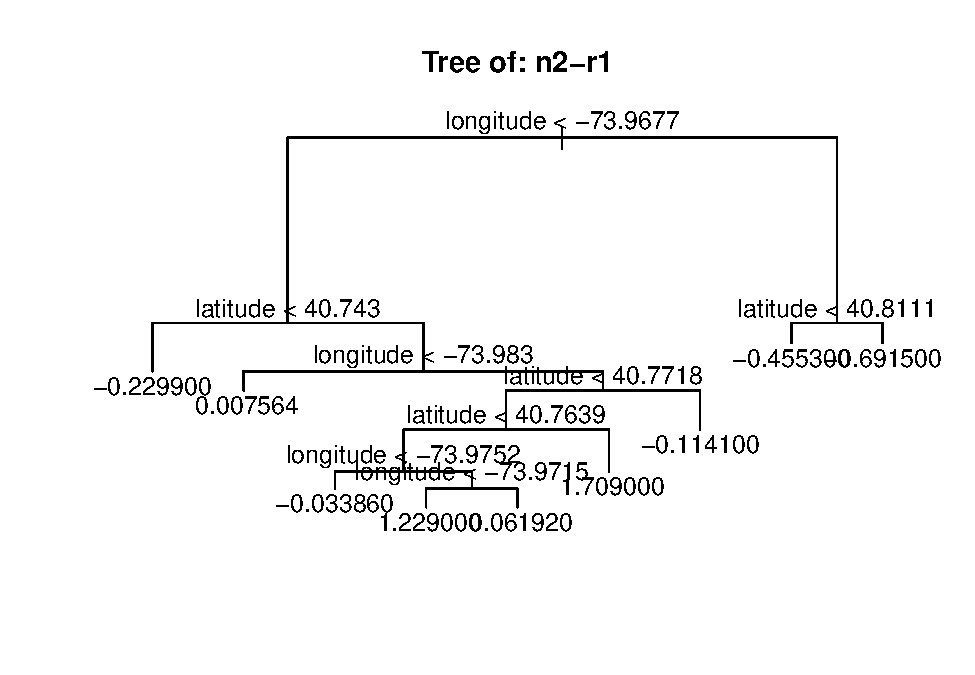
\includegraphics{project-code_files/figure-latex/unnamed-chunk-14-9.pdf}

\begin{verbatim}
## [1] 0.3753113
## 
## 
## [1] "========== n2-r2 =========="
## 
## Regression tree:
## tree(formula = price ~ ., data = trains[[sub]])
## Variables actually used in tree construction:
## [1] "longitude"
## Number of terminal nodes:  2 
## Residual mean deviance:  1.01 = 8431 / 8344 
## Distribution of residuals:
##    Min. 1st Qu.  Median    Mean 3rd Qu.    Max. 
## -2.3060 -0.7175 -0.2063  0.0000  0.4071  3.8260
\end{verbatim}

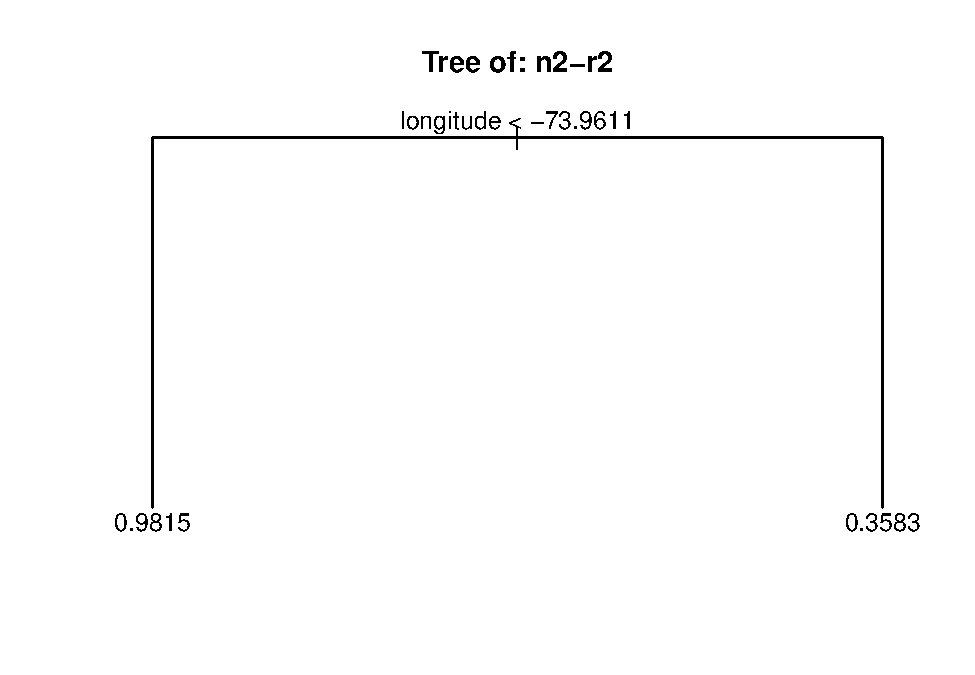
\includegraphics{project-code_files/figure-latex/unnamed-chunk-14-10.pdf}

\begin{verbatim}
## [1] 0.9585893
## 
## 
## [1] "========== n2-r3 =========="
## 
## Regression tree:
## tree(formula = price ~ ., data = trains[[sub]])
## Number of terminal nodes:  10 
## Residual mean deviance:  0.4952 = 151.5 / 306 
## Distribution of residuals:
##    Min. 1st Qu.  Median    Mean 3rd Qu.    Max. 
## -2.6830 -0.2992 -0.1347  0.0000  0.0506  3.5570
\end{verbatim}

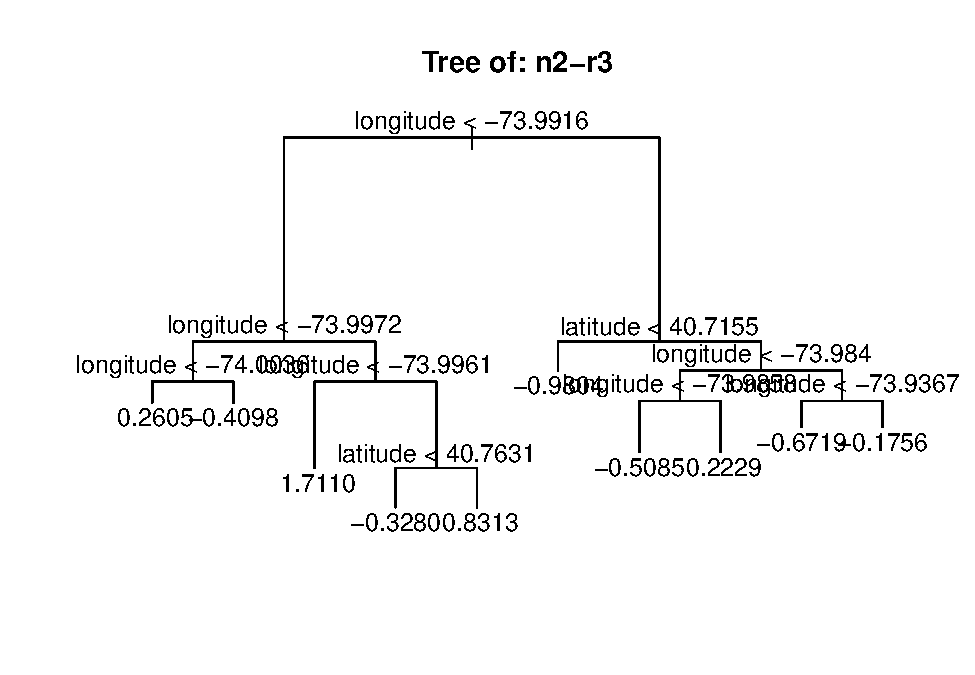
\includegraphics{project-code_files/figure-latex/unnamed-chunk-14-11.pdf}

\begin{verbatim}
## [1] 0.4992158
## 
## 
## [1] "========== n3-r1 =========="
## 
## Regression tree:
## tree(formula = price ~ ., data = trains[[sub]])
## Number of terminal nodes:  3 
## Residual mean deviance:  0.1771 = 396.5 / 2239 
## Distribution of residuals:
##     Min.  1st Qu.   Median     Mean  3rd Qu.     Max. 
## -0.88730 -0.23000 -0.08237  0.00000  0.11070  4.65500
\end{verbatim}

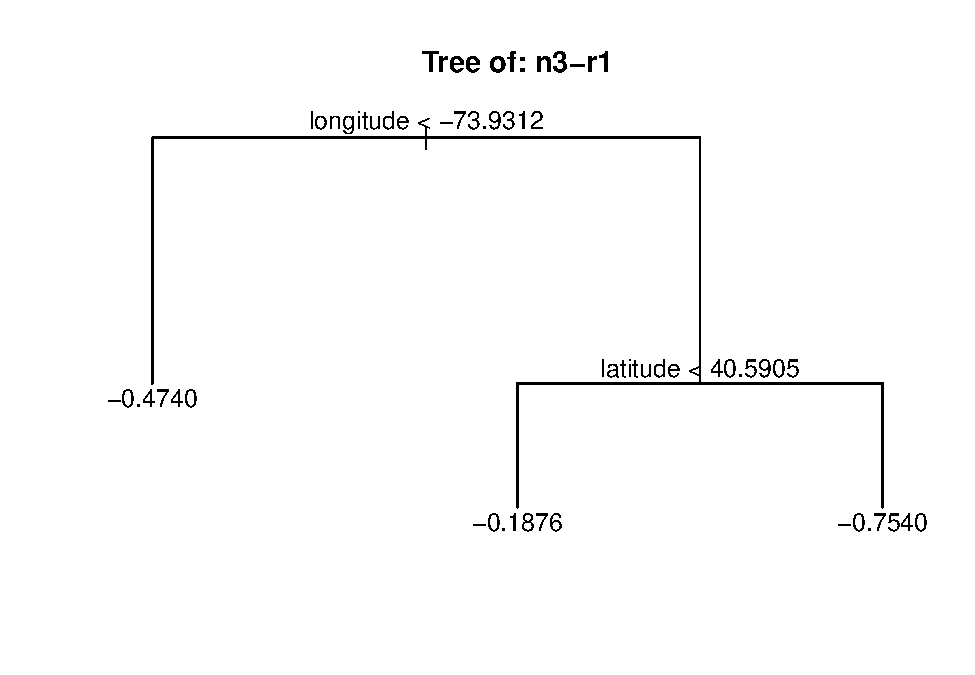
\includegraphics{project-code_files/figure-latex/unnamed-chunk-14-12.pdf}

\begin{verbatim}
## [1] 0.1551588
## 
## 
## [1] "========== n3-r2 =========="
## 
## Regression tree:
## tree(formula = price ~ ., data = trains[[sub]])
## Number of terminal nodes:  4 
## Residual mean deviance:  0.6455 = 890.9 / 1380 
## Distribution of residuals:
##    Min. 1st Qu.  Median    Mean 3rd Qu.    Max. 
## -2.1360 -0.4910 -0.2411  0.0000  0.2133  4.1890
\end{verbatim}

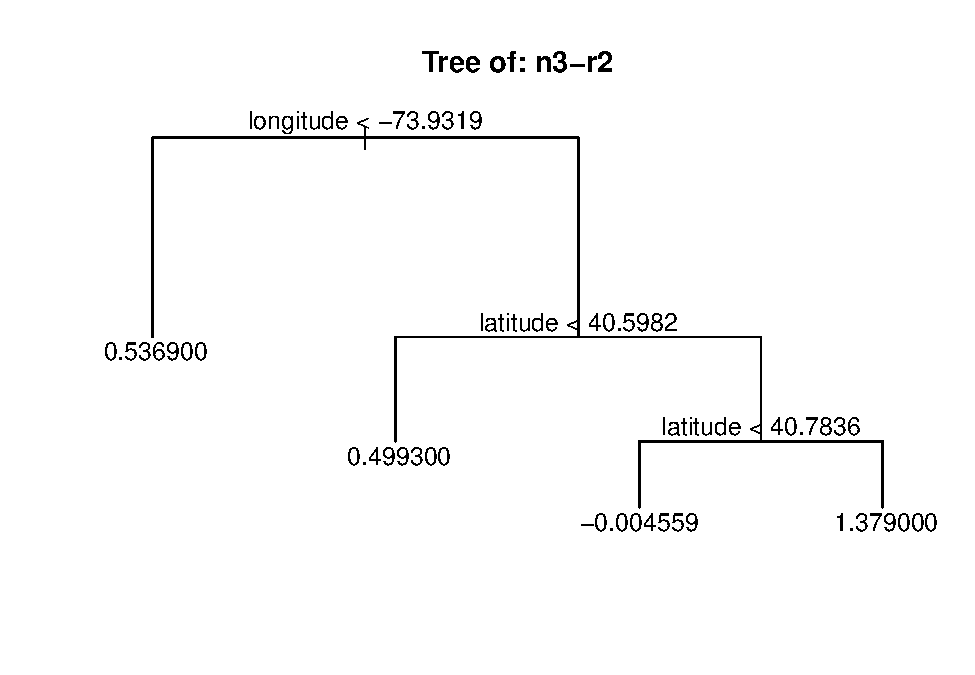
\includegraphics{project-code_files/figure-latex/unnamed-chunk-14-13.pdf}

\begin{verbatim}
## [1] 0.6995247
## 
## 
## [1] "========== n3-r3 =========="
## 
## Regression tree:
## tree(formula = price ~ ., data = trains[[sub]])
## Number of terminal nodes:  5 
## Residual mean deviance:  0.2795 = 34.65 / 124 
## Distribution of residuals:
##     Min.  1st Qu.   Median     Mean  3rd Qu.     Max. 
## -1.17100 -0.13770 -0.07213  0.00000  0.06675  4.14500
\end{verbatim}

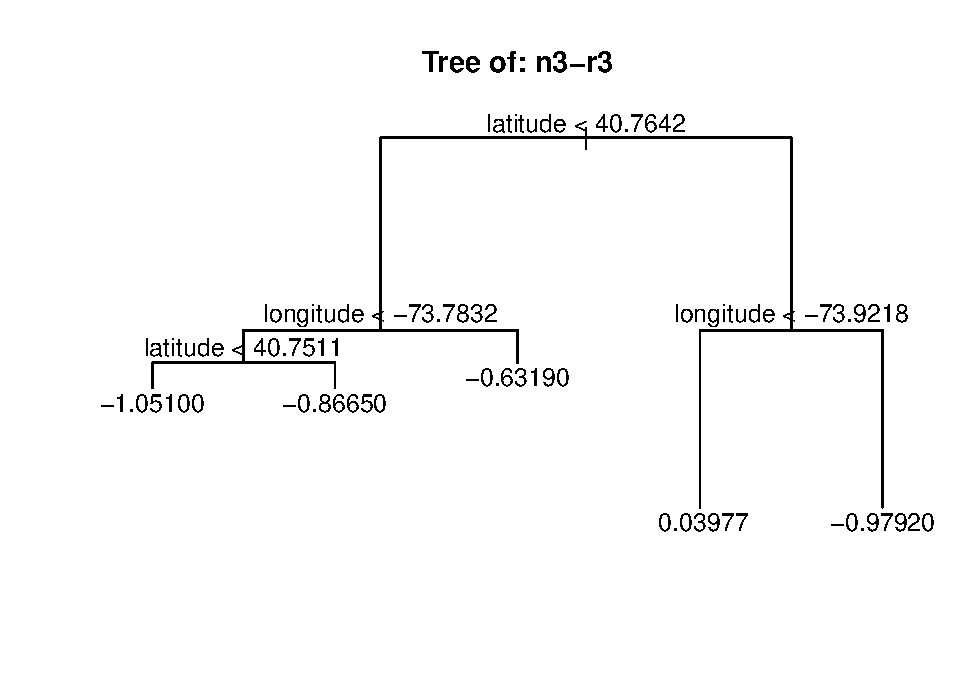
\includegraphics{project-code_files/figure-latex/unnamed-chunk-14-14.pdf}

\begin{verbatim}
## [1] 0.1667691
## 
## 
## [1] "========== n4-r1 =========="
## 
## Regression tree:
## tree(formula = price ~ ., data = trains[[sub]])
## Number of terminal nodes:  7 
## Residual mean deviance:  0.1462 = 17.4 / 119 
## Distribution of residuals:
##     Min.  1st Qu.   Median     Mean  3rd Qu.     Max. 
## -0.81560 -0.18000 -0.03524  0.00000  0.09394  2.13800
\end{verbatim}

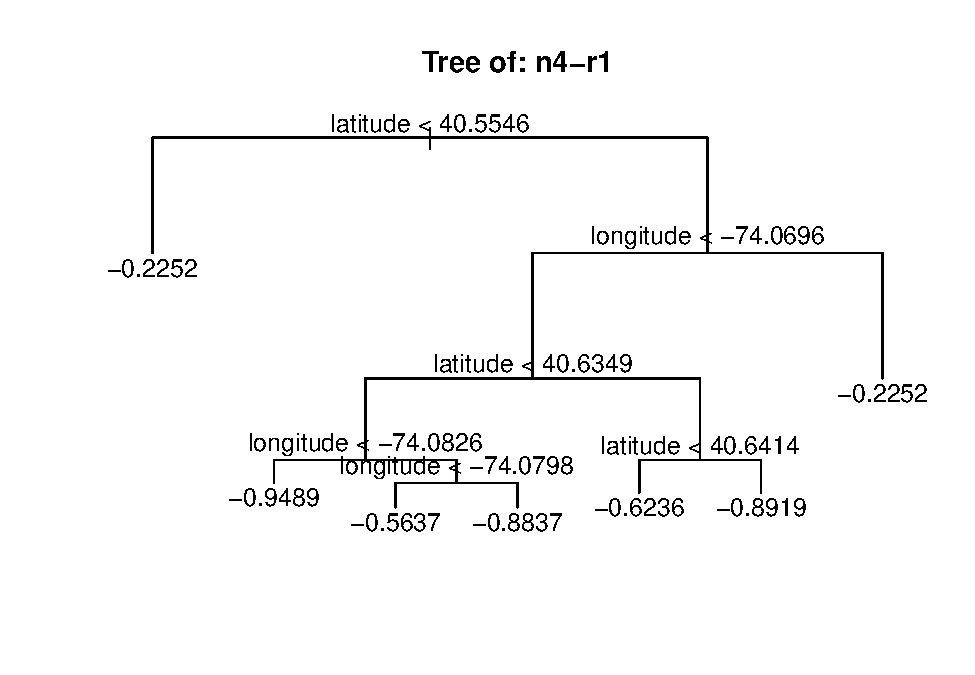
\includegraphics{project-code_files/figure-latex/unnamed-chunk-14-15.pdf}

\begin{verbatim}
## [1] 0.1605553
## 
## 
## [1] "========== n4-r2 =========="
## 
## Regression tree:
## tree(formula = price ~ ., data = trains[[sub]])
## Number of terminal nodes:  6 
## Residual mean deviance:  0.5117 = 54.76 / 107 
## Distribution of residuals:
##    Min. 1st Qu.  Median    Mean 3rd Qu.    Max. 
## -1.7900 -0.3757 -0.1485  0.0000  0.3059  2.4700
\end{verbatim}

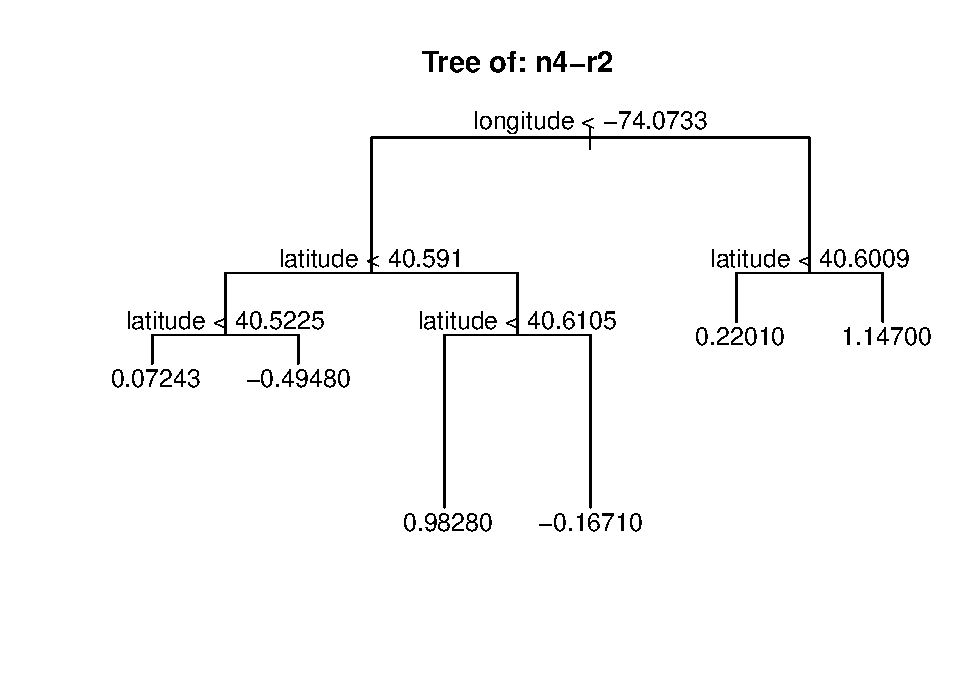
\includegraphics{project-code_files/figure-latex/unnamed-chunk-14-16.pdf}

\begin{verbatim}
## [1] 0.7737648
## 
## 
## [1] "========== n4-r3 =========="
## 
## Regression tree:
## tree(formula = price ~ ., data = trains[[sub]])
## Variables actually used in tree construction:
## character(0)
## Number of terminal nodes:  1 
## Residual mean deviance:  0.09365 = 0.3746 / 4 
## Distribution of residuals:
##    Min. 1st Qu.  Median    Mean 3rd Qu.    Max. 
## -0.2931 -0.1908 -0.1795  0.0000  0.3317  0.3317 
## Not possible to plot tree:  n4-r3[1] 0.5818964
## 
## 
## [1] "========== n5-r1 =========="
## 
## Regression tree:
## tree(formula = price ~ ., data = trains[[sub]])
## Number of terminal nodes:  5 
## Residual mean deviance:  0.163 = 69.6 / 427 
## Distribution of residuals:
##     Min.  1st Qu.   Median     Mean  3rd Qu.     Max. 
## -1.35200 -0.21400 -0.06405  0.00000  0.12680  3.81700
\end{verbatim}

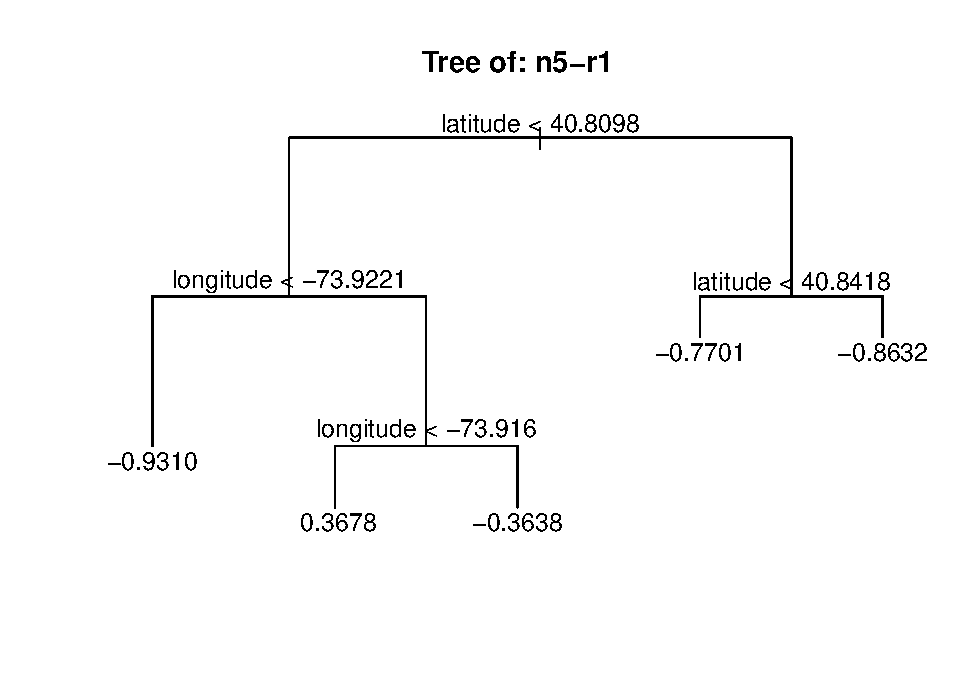
\includegraphics{project-code_files/figure-latex/unnamed-chunk-14-17.pdf}

\begin{verbatim}
## [1] 0.1611146
## 
## 
## [1] "========== n5-r2 =========="
## 
## Regression tree:
## tree(formula = price ~ ., data = trains[[sub]])
## Number of terminal nodes:  6 
## Residual mean deviance:  0.5703 = 139.7 / 245 
## Distribution of residuals:
##    Min. 1st Qu.  Median    Mean 3rd Qu.    Max. 
## -2.0970 -0.4345 -0.1505  0.0000  0.1693  3.8250
\end{verbatim}

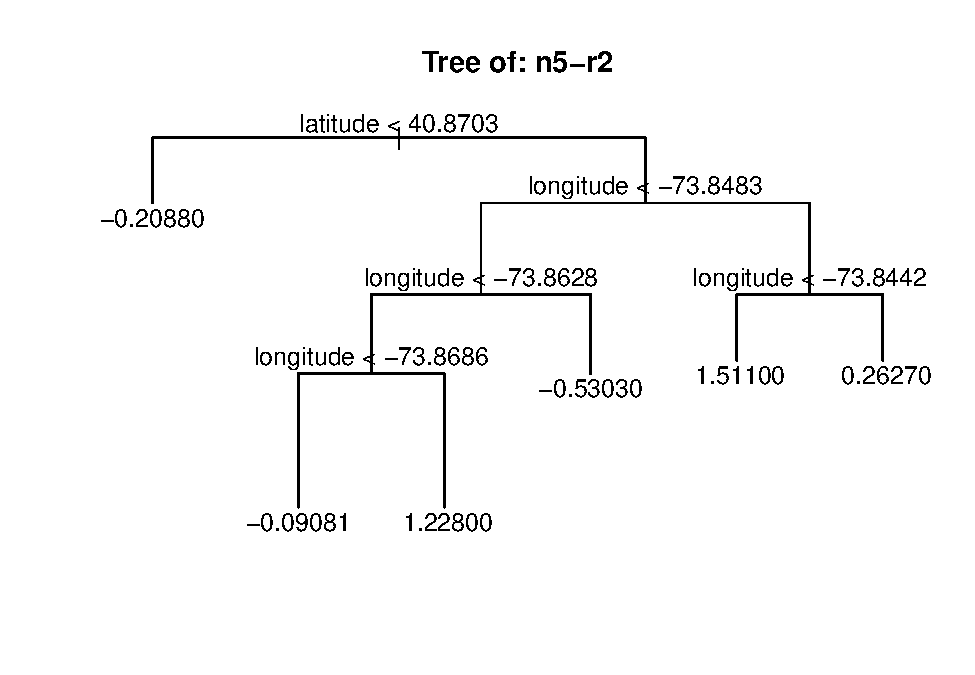
\includegraphics{project-code_files/figure-latex/unnamed-chunk-14-18.pdf}

\begin{verbatim}
## [1] 0.886004
## 
## 
## [1] "========== n5-r3 =========="
## 
## Regression tree:
## tree(formula = price ~ ., data = trains[[sub]])
## Number of terminal nodes:  5 
## Residual mean deviance:  0.07718 = 2.624 / 34 
## Distribution of residuals:
##     Min.  1st Qu.   Median     Mean  3rd Qu.     Max. 
## -0.40520 -0.17040 -0.02272  0.00000  0.04430  1.07200
\end{verbatim}

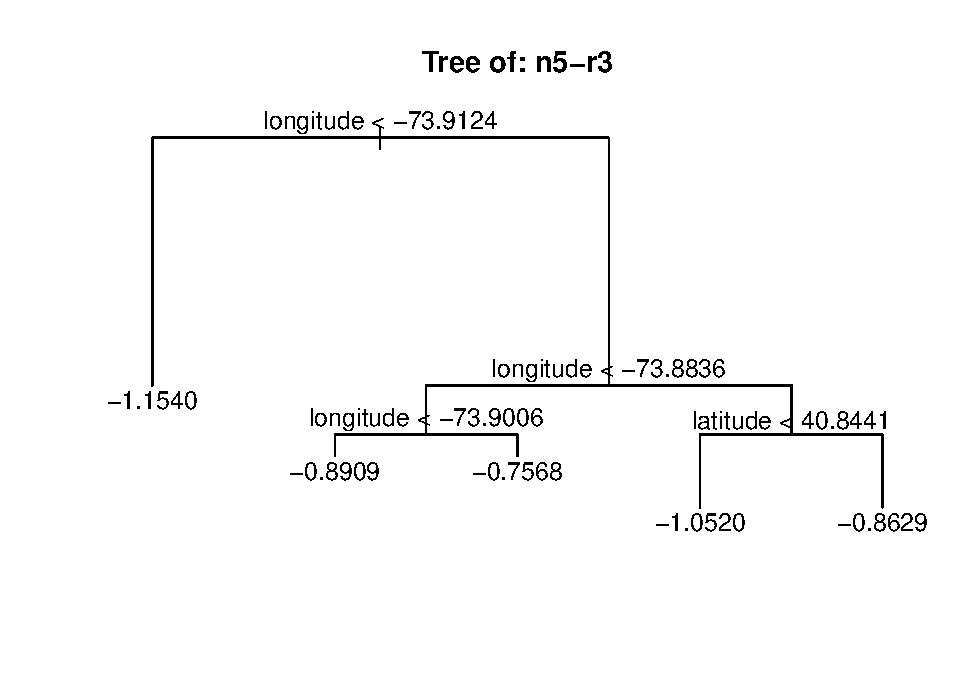
\includegraphics{project-code_files/figure-latex/unnamed-chunk-14-19.pdf}

\begin{verbatim}
## [1] 0.1939584
## 
## 
## [1] "========== all =========="
## 
## Regression tree:
## tree(formula = price ~ ., data = trains[[sub]])
## Variables actually used in tree construction:
## [1] "room_type" "longitude" "latitude" 
## Number of terminal nodes:  5 
## Residual mean deviance:  0.5997 = 17200 / 28680 
## Distribution of residuals:
##    Min. 1st Qu.  Median    Mean 3rd Qu.    Max. 
## -2.2830 -0.4196 -0.1356  0.0000  0.2166  4.8740
\end{verbatim}

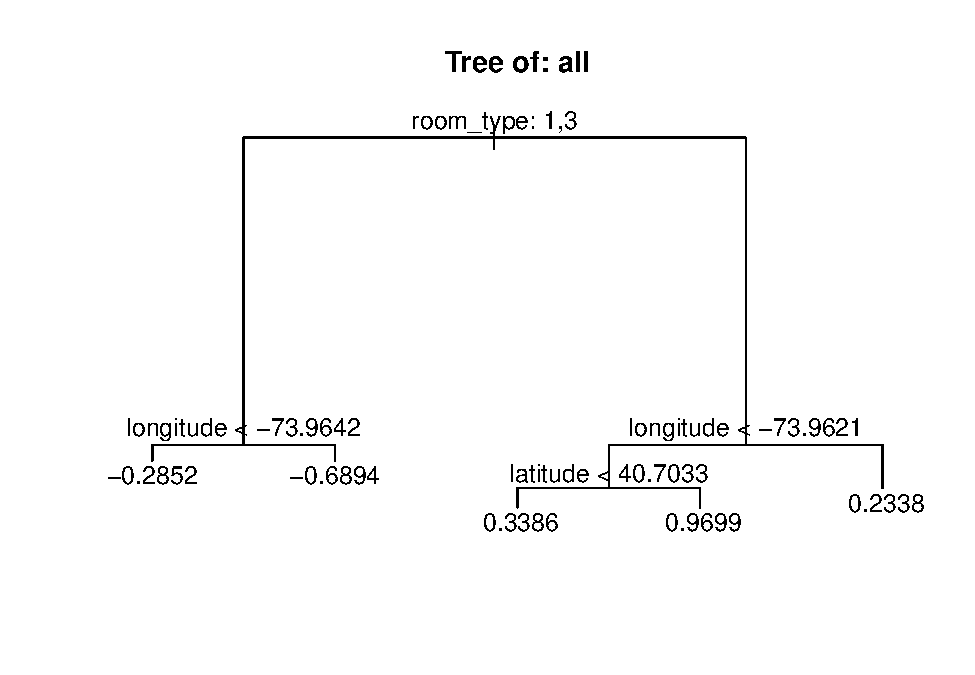
\includegraphics{project-code_files/figure-latex/unnamed-chunk-14-20.pdf}

\begin{verbatim}
## [1] 0.6149423
\end{verbatim}

\begin{Shaded}
\begin{Highlighting}[]
\NormalTok{dec_tree}\OperatorTok{$}\NormalTok{name =}\StringTok{ "Decision Tree"}
\NormalTok{model_lis}\OperatorTok{$}\NormalTok{decision_tree =}\StringTok{ }\NormalTok{dec_tree}
\end{Highlighting}
\end{Shaded}

~\\

\hypertarget{random-forest}{%
\subsection{RANDOM FOREST}\label{random-forest}}

\begin{Shaded}
\begin{Highlighting}[]
\NormalTok{rf =}\StringTok{ }\KeywordTok{vector}\NormalTok{(}\StringTok{"list"}\NormalTok{)}

\ControlFlowTok{for}\NormalTok{ (sub }\ControlFlowTok{in} \KeywordTok{names}\NormalTok{(trains))}
\NormalTok{\{}
\NormalTok{  rf[[sub]]}\OperatorTok{$}\NormalTok{fit =}\StringTok{ }\NormalTok{res =}\StringTok{  }\KeywordTok{randomForest}\NormalTok{(  price }\OperatorTok{~}\StringTok{ }\NormalTok{. , }\DataTypeTok{data=}\NormalTok{trains[[sub]])}
  
\NormalTok{  rf[[sub]]}\OperatorTok{$}\NormalTok{pred =}\StringTok{ }\NormalTok{predt =}\StringTok{ }\KeywordTok{predict}\NormalTok{(res,tests[[sub]])}
  
  \KeywordTok{print}\NormalTok{(}\KeywordTok{paste0}\NormalTok{(}\StringTok{"========== "}\NormalTok{,sub, }\StringTok{" =========="}\NormalTok{))}

  \KeywordTok{print}\NormalTok{(res)}
  
\NormalTok{  rf[[sub]]}\OperatorTok{$}\NormalTok{MSE =}\StringTok{ }\NormalTok{mse =}\StringTok{ }\KeywordTok{sum}\NormalTok{((predt }\OperatorTok{-}\StringTok{ }\NormalTok{tests[[sub]]}\OperatorTok{$}\NormalTok{price)}\OperatorTok{^}\DecValTok{2}\NormalTok{)}\OperatorTok{/}\KeywordTok{nrow}\NormalTok{(tests[[sub]])}
  \KeywordTok{print}\NormalTok{(}\KeywordTok{paste0}\NormalTok{(}\StringTok{"MSE: "}\NormalTok{,mse))}
  \KeywordTok{cat}\NormalTok{(}\StringTok{"}\CharTok{\textbackslash{}n\textbackslash{}n}\StringTok{"}\NormalTok{)}
\NormalTok{\}}
\end{Highlighting}
\end{Shaded}

\begin{verbatim}
## [1] "========== 1 =========="
## 
## Call:
##  randomForest(formula = price ~ ., data = trains[[sub]]) 
##                Type of random forest: regression
##                      Number of trees: 500
## No. of variables tried at each split: 1
## 
##           Mean of squared residuals: 0.4328756
##                     % Var explained: 41.16
## [1] "MSE: 0.437649170189599"
## 
## 
## [1] "========== 2 =========="
## 
## Call:
##  randomForest(formula = price ~ ., data = trains[[sub]]) 
##                Type of random forest: regression
##                      Number of trees: 500
## No. of variables tried at each split: 1
## 
##           Mean of squared residuals: 0.7406769
##                     % Var explained: 36.84
## [1] "MSE: 0.715054570578425"
## 
## 
## [1] "========== 3 =========="
## 
## Call:
##  randomForest(formula = price ~ ., data = trains[[sub]]) 
##                Type of random forest: regression
##                      Number of trees: 500
## No. of variables tried at each split: 1
## 
##           Mean of squared residuals: 0.3479243
##                     % Var explained: 33.31
## [1] "MSE: 0.36011180740198"
## 
## 
## [1] "========== 4 =========="
## 
## Call:
##  randomForest(formula = price ~ ., data = trains[[sub]]) 
##                Type of random forest: regression
##                      Number of trees: 500
## No. of variables tried at each split: 1
## 
##           Mean of squared residuals: 0.4166214
##                     % Var explained: 21.91
## [1] "MSE: 0.3433678508242"
## 
## 
## [1] "========== 5 =========="
## 
## Call:
##  randomForest(formula = price ~ ., data = trains[[sub]]) 
##                Type of random forest: regression
##                      Number of trees: 500
## No. of variables tried at each split: 1
## 
##           Mean of squared residuals: 0.3912467
##                     % Var explained: 21.77
## [1] "MSE: 0.271493410039648"
## 
## 
## [1] "========== n1-r1 =========="
## 
## Call:
##  randomForest(formula = price ~ ., data = trains[[sub]]) 
##                Type of random forest: regression
##                      Number of trees: 500
## No. of variables tried at each split: 1
## 
##           Mean of squared residuals: 0.1855678
##                     % Var explained: 1.89
## [1] "MSE: 0.18377381564587"
## 
## 
## [1] "========== n1-r2 =========="
## 
## Call:
##  randomForest(formula = price ~ ., data = trains[[sub]]) 
##                Type of random forest: regression
##                      Number of trees: 500
## No. of variables tried at each split: 1
## 
##           Mean of squared residuals: 0.7815159
##                     % Var explained: 2.05
## [1] "MSE: 0.801923378061946"
## 
## 
## [1] "========== n1-r3 =========="
## 
## Call:
##  randomForest(formula = price ~ ., data = trains[[sub]]) 
##                Type of random forest: regression
##                      Number of trees: 500
## No. of variables tried at each split: 1
## 
##           Mean of squared residuals: 0.1929481
##                     % Var explained: 4.76
## [1] "MSE: 0.240669947869671"
## 
## 
## [1] "========== n2-r1 =========="
## 
## Call:
##  randomForest(formula = price ~ ., data = trains[[sub]]) 
##                Type of random forest: regression
##                      Number of trees: 500
## No. of variables tried at each split: 1
## 
##           Mean of squared residuals: 0.400548
##                     % Var explained: 23.35
## [1] "MSE: 0.37844968129523"
## 
## 
## [1] "========== n2-r2 =========="
## 
## Call:
##  randomForest(formula = price ~ ., data = trains[[sub]]) 
##                Type of random forest: regression
##                      Number of trees: 500
## No. of variables tried at each split: 1
## 
##           Mean of squared residuals: 1.034235
##                     % Var explained: 4.44
## [1] "MSE: 0.977142205038175"
## 
## 
## [1] "========== n2-r3 =========="
## 
## Call:
##  randomForest(formula = price ~ ., data = trains[[sub]]) 
##                Type of random forest: regression
##                      Number of trees: 500
## No. of variables tried at each split: 1
## 
##           Mean of squared residuals: 0.7127527
##                     % Var explained: -8.63
## [1] "MSE: 0.563504335056196"
## 
## 
## [1] "========== n3-r1 =========="
## 
## Call:
##  randomForest(formula = price ~ ., data = trains[[sub]]) 
##                Type of random forest: regression
##                      Number of trees: 500
## No. of variables tried at each split: 1
## 
##           Mean of squared residuals: 0.1810658
##                     % Var explained: 1.86
## [1] "MSE: 0.151722317885811"
## 
## 
## [1] "========== n3-r2 =========="
## 
## Call:
##  randomForest(formula = price ~ ., data = trains[[sub]]) 
##                Type of random forest: regression
##                      Number of trees: 500
## No. of variables tried at each split: 1
## 
##           Mean of squared residuals: 0.6678137
##                     % Var explained: 2.11
## [1] "MSE: 0.713578829161869"
## 
## 
## [1] "========== n3-r3 =========="
## 
## Call:
##  randomForest(formula = price ~ ., data = trains[[sub]]) 
##                Type of random forest: regression
##                      Number of trees: 500
## No. of variables tried at each split: 1
## 
##           Mean of squared residuals: 0.4066588
##                     % Var explained: -19.19
## [1] "MSE: 0.222952585446267"
## 
## 
## [1] "========== n4-r1 =========="
## 
## Call:
##  randomForest(formula = price ~ ., data = trains[[sub]]) 
##                Type of random forest: regression
##                      Number of trees: 500
## No. of variables tried at each split: 1
## 
##           Mean of squared residuals: 0.1895889
##                     % Var explained: -2.23
## [1] "MSE: 0.14235780616274"
## 
## 
## [1] "========== n4-r2 =========="
## 
## Call:
##  randomForest(formula = price ~ ., data = trains[[sub]]) 
##                Type of random forest: regression
##                      Number of trees: 500
## No. of variables tried at each split: 1
## 
##           Mean of squared residuals: 0.7799421
##                     % Var explained: -15.53
## [1] "MSE: 0.71895373565863"
\end{verbatim}

\begin{verbatim}
## Warning in randomForest.default(m, y, ...): The response has five or fewer
## unique values. Are you sure you want to do regression?
\end{verbatim}

\begin{verbatim}
## [1] "========== n4-r3 =========="
## 
## Call:
##  randomForest(formula = price ~ ., data = trains[[sub]]) 
##                Type of random forest: regression
##                      Number of trees: 500
## No. of variables tried at each split: 1
## 
##           Mean of squared residuals: 0.0182975
##                     % Var explained: 75.58
## [1] "MSE: 0.303227871154577"
## 
## 
## [1] "========== n5-r1 =========="
## 
## Call:
##  randomForest(formula = price ~ ., data = trains[[sub]]) 
##                Type of random forest: regression
##                      Number of trees: 500
## No. of variables tried at each split: 1
## 
##           Mean of squared residuals: 0.2109273
##                     % Var explained: -15.99
## [1] "MSE: 0.133084811823872"
## 
## 
## [1] "========== n5-r2 =========="
## 
## Call:
##  randomForest(formula = price ~ ., data = trains[[sub]]) 
##                Type of random forest: regression
##                      Number of trees: 500
## No. of variables tried at each split: 1
## 
##           Mean of squared residuals: 0.726527
##                     % Var explained: -6.48
## [1] "MSE: 0.870094681564989"
## 
## 
## [1] "========== n5-r3 =========="
## 
## Call:
##  randomForest(formula = price ~ ., data = trains[[sub]]) 
##                Type of random forest: regression
##                      Number of trees: 500
## No. of variables tried at each split: 1
## 
##           Mean of squared residuals: 0.1083252
##                     % Var explained: -22.7
## [1] "MSE: 0.176332867102828"
## 
## 
## [1] "========== all =========="
## 
## Call:
##  randomForest(formula = price ~ ., data = trains[[sub]]) 
##                Type of random forest: regression
##                      Number of trees: 500
## No. of variables tried at each split: 1
## 
##           Mean of squared residuals: 0.5704246
##                     % Var explained: 42.45
## [1] "MSE: 0.58523248835968"
\end{verbatim}

\begin{Shaded}
\begin{Highlighting}[]
\NormalTok{rf}\OperatorTok{$}\NormalTok{name =}\StringTok{ "Random Forest"}
\NormalTok{model_lis}\OperatorTok{$}\NormalTok{random_forest =}\StringTok{ }\NormalTok{rf}
\end{Highlighting}
\end{Shaded}

~\\

\hypertarget{ranger-random-forest}{%
\subsection{RANGER RANDOM FOREST}\label{ranger-random-forest}}

\begin{Shaded}
\begin{Highlighting}[]
\NormalTok{ranger_rf =}\StringTok{ }\KeywordTok{vector}\NormalTok{(}\StringTok{"list"}\NormalTok{)}

\ControlFlowTok{for}\NormalTok{ (sub }\ControlFlowTok{in} \KeywordTok{names}\NormalTok{(trains))}
\NormalTok{\{}
  
   \KeywordTok{print}\NormalTok{(}\KeywordTok{paste0}\NormalTok{(}\StringTok{"========== "}\NormalTok{,sub, }\StringTok{" =========="}\NormalTok{))}

\NormalTok{  ranger_rf[[sub]]}\OperatorTok{$}\NormalTok{fit =}\StringTok{ }\NormalTok{res =}\StringTok{ }\KeywordTok{ranger}\NormalTok{( price}\OperatorTok{~}\StringTok{ }\NormalTok{., }\DataTypeTok{data =}\NormalTok{ trains[[sub]], }\DataTypeTok{write.forest =} \OtherTok{TRUE}\NormalTok{, }\DataTypeTok{classification =}\NormalTok{ F)}
  
\NormalTok{  ranger_rf[[sub]]}\OperatorTok{$}\NormalTok{pred =}\StringTok{ }\NormalTok{predt =}\StringTok{ }\KeywordTok{predict}\NormalTok{(res,tests[[sub]])}
\NormalTok{  ranger_rf[[sub]]}\OperatorTok{$}\NormalTok{MSE =}\StringTok{ }\NormalTok{mse =}\StringTok{  }\KeywordTok{sum}\NormalTok{((predt}\OperatorTok{$}\NormalTok{predictions }\OperatorTok{-}\StringTok{ }\NormalTok{tests[[sub]]}\OperatorTok{$}\NormalTok{price)}\OperatorTok{^}\DecValTok{2}\NormalTok{)}\OperatorTok{/}\KeywordTok{nrow}\NormalTok{(tests[[sub]])}
  \KeywordTok{print}\NormalTok{(res)}
  \KeywordTok{print}\NormalTok{(}\KeywordTok{paste0}\NormalTok{(}\StringTok{"MSE: "}\NormalTok{,mse))}
  \KeywordTok{cat}\NormalTok{(}\StringTok{"}\CharTok{\textbackslash{}n\textbackslash{}n}\StringTok{"}\NormalTok{)}
\NormalTok{\}}
\end{Highlighting}
\end{Shaded}

\begin{verbatim}
## [1] "========== 1 =========="
## Ranger result
## 
## Call:
##  ranger(price ~ ., data = trains[[sub]], write.forest = TRUE,      classification = F) 
## 
## Type:                             Regression 
## Number of trees:                  500 
## Sample size:                      14893 
## Number of independent variables:  3 
## Mtry:                             1 
## Target node size:                 5 
## Variable importance mode:         none 
## Splitrule:                        variance 
## OOB prediction error (MSE):       0.4300719 
## R squared (OOB):                  0.4154151 
## [1] "MSE: 0.435661195179693"
## 
## 
## [1] "========== 2 =========="
## Ranger result
## 
## Call:
##  ranger(price ~ ., data = trains[[sub]], write.forest = TRUE,      classification = F) 
## 
## Type:                             Regression 
## Number of trees:                  500 
## Sample size:                      15658 
## Number of independent variables:  3 
## Mtry:                             1 
## Target node size:                 5 
## Variable importance mode:         none 
## Splitrule:                        variance 
## OOB prediction error (MSE):       0.7402947 
## R squared (OOB):                  0.368762 
## [1] "MSE: 0.713232260548964"
## 
## 
## [1] "========== 3 =========="
## Ranger result
## 
## Call:
##  ranger(price ~ ., data = trains[[sub]], write.forest = TRUE,      classification = F) 
## 
## Type:                             Regression 
## Number of trees:                  500 
## Sample size:                      4224 
## Number of independent variables:  3 
## Mtry:                             1 
## Target node size:                 5 
## Variable importance mode:         none 
## Splitrule:                        variance 
## OOB prediction error (MSE):       0.3469485 
## R squared (OOB):                  0.3351217 
## [1] "MSE: 0.359439894738383"
## 
## 
## [1] "========== 4 =========="
## Ranger result
## 
## Call:
##  ranger(price ~ ., data = trains[[sub]], write.forest = TRUE,      classification = F) 
## 
## Type:                             Regression 
## Number of trees:                  500 
## Sample size:                      274 
## Number of independent variables:  3 
## Mtry:                             1 
## Target node size:                 5 
## Variable importance mode:         none 
## Splitrule:                        variance 
## OOB prediction error (MSE):       0.4235784 
## R squared (OOB):                  0.208931 
## [1] "MSE: 0.349825116770277"
## 
## 
## [1] "========== 5 =========="
## Ranger result
## 
## Call:
##  ranger(price ~ ., data = trains[[sub]], write.forest = TRUE,      classification = F) 
## 
## Type:                             Regression 
## Number of trees:                  500 
## Sample size:                      811 
## Number of independent variables:  3 
## Mtry:                             1 
## Target node size:                 5 
## Variable importance mode:         none 
## Splitrule:                        variance 
## OOB prediction error (MSE):       0.3985611 
## R squared (OOB):                  0.2040182 
## [1] "MSE: 0.268062661260826"
## 
## 
## [1] "========== n1-r1 =========="
## Ranger result
## 
## Call:
##  ranger(price ~ ., data = trains[[sub]], write.forest = TRUE,      classification = F) 
## 
## Type:                             Regression 
## Number of trees:                  500 
## Sample size:                      6724 
## Number of independent variables:  2 
## Mtry:                             1 
## Target node size:                 5 
## Variable importance mode:         none 
## Splitrule:                        variance 
## OOB prediction error (MSE):       0.1858047 
## R squared (OOB):                  0.01779825 
## [1] "MSE: 0.183050763664203"
## 
## 
## [1] "========== n1-r2 =========="
## Ranger result
## 
## Call:
##  ranger(price ~ ., data = trains[[sub]], write.forest = TRUE,      classification = F) 
## 
## Type:                             Regression 
## Number of trees:                  500 
## Sample size:                      6241 
## Number of independent variables:  2 
## Mtry:                             1 
## Target node size:                 5 
## Variable importance mode:         none 
## Splitrule:                        variance 
## OOB prediction error (MSE):       0.7820273 
## R squared (OOB):                  0.02001014 
## [1] "MSE: 0.805646710986738"
## 
## 
## [1] "========== n1-r3 =========="
## Ranger result
## 
## Call:
##  ranger(price ~ ., data = trains[[sub]], write.forest = TRUE,      classification = F) 
## 
## Type:                             Regression 
## Number of trees:                  500 
## Sample size:                      273 
## Number of independent variables:  2 
## Mtry:                             1 
## Target node size:                 5 
## Variable importance mode:         none 
## Splitrule:                        variance 
## OOB prediction error (MSE):       0.1935494 
## R squared (OOB):                  0.04816971 
## [1] "MSE: 0.238626751943499"
## 
## 
## [1] "========== n2-r1 =========="
## Ranger result
## 
## Call:
##  ranger(price ~ ., data = trains[[sub]], write.forest = TRUE,      classification = F) 
## 
## Type:                             Regression 
## Number of trees:                  500 
## Sample size:                      5255 
## Number of independent variables:  2 
## Mtry:                             1 
## Target node size:                 5 
## Variable importance mode:         none 
## Splitrule:                        variance 
## OOB prediction error (MSE):       0.3999019 
## R squared (OOB):                  0.2348782 
## [1] "MSE: 0.378283997644987"
## 
## 
## [1] "========== n2-r2 =========="
## Ranger result
## 
## Call:
##  ranger(price ~ ., data = trains[[sub]], write.forest = TRUE,      classification = F) 
## 
## Type:                             Regression 
## Number of trees:                  500 
## Sample size:                      8346 
## Number of independent variables:  2 
## Mtry:                             1 
## Target node size:                 5 
## Variable importance mode:         none 
## Splitrule:                        variance 
## OOB prediction error (MSE):       1.036799 
## R squared (OOB):                  0.04214508 
## [1] "MSE: 0.974357995618573"
## 
## 
## [1] "========== n2-r3 =========="
## Ranger result
## 
## Call:
##  ranger(price ~ ., data = trains[[sub]], write.forest = TRUE,      classification = F) 
## 
## Type:                             Regression 
## Number of trees:                  500 
## Sample size:                      316 
## Number of independent variables:  2 
## Mtry:                             1 
## Target node size:                 5 
## Variable importance mode:         none 
## Splitrule:                        variance 
## OOB prediction error (MSE):       0.7160939 
## R squared (OOB):                  -0.08798569 
## [1] "MSE: 0.57155262780546"
## 
## 
## [1] "========== n3-r1 =========="
## Ranger result
## 
## Call:
##  ranger(price ~ ., data = trains[[sub]], write.forest = TRUE,      classification = F) 
## 
## Type:                             Regression 
## Number of trees:                  500 
## Sample size:                      2242 
## Number of independent variables:  2 
## Mtry:                             1 
## Target node size:                 5 
## Variable importance mode:         none 
## Splitrule:                        variance 
## OOB prediction error (MSE):       0.181763 
## R squared (OOB):                  0.01525706 
## [1] "MSE: 0.152704198115273"
## 
## 
## [1] "========== n3-r2 =========="
## Ranger result
## 
## Call:
##  ranger(price ~ ., data = trains[[sub]], write.forest = TRUE,      classification = F) 
## 
## Type:                             Regression 
## Number of trees:                  500 
## Sample size:                      1384 
## Number of independent variables:  2 
## Mtry:                             1 
## Target node size:                 5 
## Variable importance mode:         none 
## Splitrule:                        variance 
## OOB prediction error (MSE):       0.6704211 
## R squared (OOB):                  0.01803546 
## [1] "MSE: 0.71238608718685"
## 
## 
## [1] "========== n3-r3 =========="
## Ranger result
## 
## Call:
##  ranger(price ~ ., data = trains[[sub]], write.forest = TRUE,      classification = F) 
## 
## Type:                             Regression 
## Number of trees:                  500 
## Sample size:                      129 
## Number of independent variables:  2 
## Mtry:                             1 
## Target node size:                 5 
## Variable importance mode:         none 
## Splitrule:                        variance 
## OOB prediction error (MSE):       0.4162768 
## R squared (OOB):                  -0.2106128 
## [1] "MSE: 0.22139444129044"
## 
## 
## [1] "========== n4-r1 =========="
## Ranger result
## 
## Call:
##  ranger(price ~ ., data = trains[[sub]], write.forest = TRUE,      classification = F) 
## 
## Type:                             Regression 
## Number of trees:                  500 
## Sample size:                      126 
## Number of independent variables:  2 
## Mtry:                             1 
## Target node size:                 5 
## Variable importance mode:         none 
## Splitrule:                        variance 
## OOB prediction error (MSE):       0.1911728 
## R squared (OOB):                  -0.02263984 
## [1] "MSE: 0.143390186091069"
## 
## 
## [1] "========== n4-r2 =========="
## Ranger result
## 
## Call:
##  ranger(price ~ ., data = trains[[sub]], write.forest = TRUE,      classification = F) 
## 
## Type:                             Regression 
## Number of trees:                  500 
## Sample size:                      113 
## Number of independent variables:  2 
## Mtry:                             1 
## Target node size:                 5 
## Variable importance mode:         none 
## Splitrule:                        variance 
## OOB prediction error (MSE):       0.7852717 
## R squared (OOB):                  -0.1528912 
## [1] "MSE: 0.705639717093316"
## 
## 
## [1] "========== n4-r3 =========="
## Ranger result
## 
## Call:
##  ranger(price ~ ., data = trains[[sub]], write.forest = TRUE,      classification = F) 
## 
## Type:                             Regression 
## Number of trees:                  500 
## Sample size:                      5 
## Number of independent variables:  2 
## Mtry:                             1 
## Target node size:                 5 
## Variable importance mode:         none 
## Splitrule:                        variance 
## OOB prediction error (MSE):       0.1158974 
## R squared (OOB):                  -0.2376012 
## [1] "MSE: 0.584749620286946"
## 
## 
## [1] "========== n5-r1 =========="
## Ranger result
## 
## Call:
##  ranger(price ~ ., data = trains[[sub]], write.forest = TRUE,      classification = F) 
## 
## Type:                             Regression 
## Number of trees:                  500 
## Sample size:                      432 
## Number of independent variables:  2 
## Mtry:                             1 
## Target node size:                 5 
## Variable importance mode:         none 
## Splitrule:                        variance 
## OOB prediction error (MSE):       0.2150884 
## R squared (OOB):                  -0.1800232 
## [1] "MSE: 0.132753624265668"
## 
## 
## [1] "========== n5-r2 =========="
## Ranger result
## 
## Call:
##  ranger(price ~ ., data = trains[[sub]], write.forest = TRUE,      classification = F) 
## 
## Type:                             Regression 
## Number of trees:                  500 
## Sample size:                      251 
## Number of independent variables:  2 
## Mtry:                             1 
## Target node size:                 5 
## Variable importance mode:         none 
## Splitrule:                        variance 
## OOB prediction error (MSE):       0.7310383 
## R squared (OOB):                  -0.06716958 
## [1] "MSE: 0.870872319133183"
## 
## 
## [1] "========== n5-r3 =========="
## Ranger result
## 
## Call:
##  ranger(price ~ ., data = trains[[sub]], write.forest = TRUE,      classification = F) 
## 
## Type:                             Regression 
## Number of trees:                  500 
## Sample size:                      39 
## Number of independent variables:  2 
## Mtry:                             1 
## Target node size:                 5 
## Variable importance mode:         none 
## Splitrule:                        variance 
## OOB prediction error (MSE):       0.1122889 
## R squared (OOB):                  -0.2393209 
## [1] "MSE: 0.17684139550054"
## 
## 
## [1] "========== all =========="
## Ranger result
## 
## Call:
##  ranger(price ~ ., data = trains[[sub]], write.forest = TRUE,      classification = F) 
## 
## Type:                             Regression 
## Number of trees:                  500 
## Sample size:                      28689 
## Number of independent variables:  4 
## Mtry:                             2 
## Target node size:                 5 
## Variable importance mode:         none 
## Splitrule:                        variance 
## OOB prediction error (MSE):       0.5431618 
## R squared (OOB):                  0.4520079 
## [1] "MSE: 0.553992505569662"
\end{verbatim}

\begin{Shaded}
\begin{Highlighting}[]
\NormalTok{ranger_rf}\OperatorTok{$}\NormalTok{name =}\StringTok{ "Ranger Random Forest"}
\NormalTok{model_lis}\OperatorTok{$}\NormalTok{ranger =}\StringTok{ }\NormalTok{ranger_rf}
\end{Highlighting}
\end{Shaded}

~\\

\hypertarget{neural-networks}{%
\subsection{NEURAL NETWORKS}\label{neural-networks}}

\begin{Shaded}
\begin{Highlighting}[]
\NormalTok{build_model <-}\StringTok{ }\ControlFlowTok{function}\NormalTok{(dimension) \{}
  
\NormalTok{  model <-}\StringTok{ }\NormalTok{keras}\OperatorTok{::}\KeywordTok{keras_model_sequential}\NormalTok{() }\OperatorTok
\StringTok{    }\KeywordTok{layer_dense}\NormalTok{(}\DataTypeTok{units =} \DecValTok{32}\NormalTok{, }\DataTypeTok{activation =} \StringTok{"relu"}\NormalTok{,}
                \DataTypeTok{input_shape =}\NormalTok{ dimension) }\OperatorTok
\StringTok{    }\KeywordTok{layer_dense}\NormalTok{(}\DataTypeTok{units =} \DecValTok{16}\NormalTok{, }\DataTypeTok{activation =} \StringTok{"relu"}\NormalTok{) }\OperatorTok
\StringTok{    }\KeywordTok{layer_dense}\NormalTok{(}\DataTypeTok{units =} \DecValTok{1}\NormalTok{,}\DataTypeTok{activation=}\StringTok{"linear"}\NormalTok{)}
  
\NormalTok{  model }\OperatorTok\StringTok{ }\KeywordTok{compile}\NormalTok{(}
    \DataTypeTok{loss =} \StringTok{"mse"}\NormalTok{,}
    \DataTypeTok{optimizer =} \KeywordTok{optimizer_rmsprop}\NormalTok{(),}
    \DataTypeTok{metrics =} \KeywordTok{list}\NormalTok{(}\StringTok{"mean_absolute_error"}\NormalTok{)}
\NormalTok{  )}
  
  \KeywordTok{return}\NormalTok{(model)}
\NormalTok{\}}


\NormalTok{print_dot_callback <-}\StringTok{ }\KeywordTok{callback_lambda}\NormalTok{(}
  \DataTypeTok{on_epoch_end =} \ControlFlowTok{function}\NormalTok{(epoch, logs) \{}
    \ControlFlowTok{if}\NormalTok{ (epoch }\OperatorTok\StringTok{ }\DecValTok{1} \OperatorTok{==}\StringTok{ }\DecValTok{0}\NormalTok{) }
      \KeywordTok{cat}\NormalTok{(}\StringTok{"."}\NormalTok{)}
\NormalTok{  \}}
\NormalTok{)    }


\NormalTok{nn =}\StringTok{ }\KeywordTok{vector}\NormalTok{(}\StringTok{"list"}\NormalTok{)}

\ControlFlowTok{for}\NormalTok{ (sub }\ControlFlowTok{in} \KeywordTok{names}\NormalTok{(trains))}
\NormalTok{\{}
\NormalTok{  d =}\StringTok{ }\NormalTok{trains[[sub]]}
\NormalTok{  d2 =}\StringTok{ }\NormalTok{tests[[sub]]}
\NormalTok{  len =}\StringTok{ }\KeywordTok{length}\NormalTok{(d)}
\NormalTok{  len2 =}\StringTok{ }\KeywordTok{length}\NormalTok{(d2)}
  
  \ControlFlowTok{if}\NormalTok{(}\OperatorTok{!}\KeywordTok{is.null}\NormalTok{(d}\OperatorTok{$}\NormalTok{room_type))}
\NormalTok{  \{}
\NormalTok{    d}\OperatorTok{$}\NormalTok{room_type =}\StringTok{ }\NormalTok{keras}\OperatorTok{::}\KeywordTok{to_categorical}\NormalTok{(d}\OperatorTok{$}\NormalTok{room_type)}
\NormalTok{    d2}\OperatorTok{$}\NormalTok{room_type =}\StringTok{ }\NormalTok{keras}\OperatorTok{::}\KeywordTok{to_categorical}\NormalTok{(d2}\OperatorTok{$}\NormalTok{room_type)}
    
\NormalTok{  \}}
  
  \ControlFlowTok{if}\NormalTok{(}\OperatorTok{!}\KeywordTok{is.null}\NormalTok{(d}\OperatorTok{$}\NormalTok{neighbourhood_group)) }
\NormalTok{  \{}
\NormalTok{    d}\OperatorTok{$}\NormalTok{neighbourhood_group =}\StringTok{ }\NormalTok{keras}\OperatorTok{::}\KeywordTok{to_categorical}\NormalTok{(d}\OperatorTok{$}\NormalTok{neighbourhood_group)}
\NormalTok{    d2}\OperatorTok{$}\NormalTok{neighbourhood_group =}\StringTok{ }\NormalTok{keras}\OperatorTok{::}\KeywordTok{to_categorical}\NormalTok{(d2}\OperatorTok{$}\NormalTok{neighbourhood_group)}
\NormalTok{  \}}
  
  
\NormalTok{  target =}\StringTok{ }\KeywordTok{as.vector}\NormalTok{(d}\OperatorTok{$}\NormalTok{price)}
\NormalTok{  features =}\StringTok{ }\KeywordTok{as.matrix}\NormalTok{(}\KeywordTok{as_tibble}\NormalTok{(d[}\OperatorTok{-}\NormalTok{len]))}
  
\NormalTok{  target_test =}\StringTok{ }\KeywordTok{as.vector}\NormalTok{(d2}\OperatorTok{$}\NormalTok{price)}
\NormalTok{  features_test =}\StringTok{ }\KeywordTok{as.matrix}\NormalTok{(}\KeywordTok{as_tibble}\NormalTok{(d2[}\OperatorTok{-}\NormalTok{len]))}
  
  
\NormalTok{  nn[[sub]]}\OperatorTok{$}\NormalTok{epochs =}\StringTok{ }\NormalTok{epochs =}\StringTok{  }\DecValTok{30}
  
\NormalTok{  nn[[sub]]}\OperatorTok{$}\NormalTok{model =}\StringTok{ }\NormalTok{model =}\StringTok{  }\KeywordTok{build_model}\NormalTok{(}\KeywordTok{dim}\NormalTok{(features)[}\DecValTok{2}\NormalTok{])}
  
\NormalTok{  nn[[sub]]}\OperatorTok{$}\NormalTok{summary =}\StringTok{ }\NormalTok{model }\OperatorTok\StringTok{ }\KeywordTok{summary}\NormalTok{()}
\NormalTok{  nn[[sub]]}\OperatorTok{$}\NormalTok{history =}\StringTok{ }\NormalTok{hist =}\StringTok{  }\NormalTok{model }\OperatorTok\StringTok{ }\KeywordTok{fit}\NormalTok{(}
    \DataTypeTok{x =}\NormalTok{ features,}
    \DataTypeTok{y =}\NormalTok{ target,}
    \DataTypeTok{epochs =}\NormalTok{ epochs,}
    \DataTypeTok{validation_split =} \FloatTok{0.2}\NormalTok{,}
    \DataTypeTok{verbose =} \DecValTok{0}\NormalTok{,}
    \DataTypeTok{callbacks =} \KeywordTok{list}\NormalTok{(print_dot_callback)}
\NormalTok{  )}
\NormalTok{  eva =}\StringTok{ }\NormalTok{model }\OperatorTok\StringTok{ }\KeywordTok{evaluate}\NormalTok{(features_test,target_test, }\DataTypeTok{verbose =} \DecValTok{0}\NormalTok{)}
  
  
\NormalTok{  nn[[sub]]}\OperatorTok{$}\NormalTok{mae =}\StringTok{ }\NormalTok{eva[}\DecValTok{1}\NormalTok{]}
\NormalTok{  nn[[sub]]}\OperatorTok{$}\NormalTok{loss =}\StringTok{ }\NormalTok{eva[}\DecValTok{2}\NormalTok{]}
  
\NormalTok{  nn[[sub]]}\OperatorTok{$}\NormalTok{pred =}\StringTok{ }\NormalTok{pred =}\StringTok{ }\NormalTok{model }\OperatorTok\StringTok{ }\KeywordTok{predict}\NormalTok{(features_test)}
\NormalTok{  nn[[sub]]}\OperatorTok{$}\NormalTok{MSE =}\StringTok{ }\KeywordTok{sum}\NormalTok{((pred }\OperatorTok{-}\StringTok{ }\NormalTok{target_test)}\OperatorTok{^}\DecValTok{2}\NormalTok{)}\OperatorTok{/}\KeywordTok{length}\NormalTok{(target_test)}
  
\NormalTok{\}}
\end{Highlighting}
\end{Shaded}

\begin{verbatim}
## Model: "sequential"
## ________________________________________________________________________________
## Layer (type)                        Output Shape                    Param #     
## ================================================================================
## dense (Dense)                       (None, 32)                      224         
## ________________________________________________________________________________
## dense_1 (Dense)                     (None, 16)                      528         
## ________________________________________________________________________________
## dense_2 (Dense)                     (None, 1)                       17          
## ================================================================================
## Total params: 769
## Trainable params: 769
## Non-trainable params: 0
## ________________________________________________________________________________
## ..............................Model: "sequential_1"
## ________________________________________________________________________________
## Layer (type)                        Output Shape                    Param #     
## ================================================================================
## dense_3 (Dense)                     (None, 32)                      224         
## ________________________________________________________________________________
## dense_4 (Dense)                     (None, 16)                      528         
## ________________________________________________________________________________
## dense_5 (Dense)                     (None, 1)                       17          
## ================================================================================
## Total params: 769
## Trainable params: 769
## Non-trainable params: 0
## ________________________________________________________________________________
## ..............................Model: "sequential_2"
## ________________________________________________________________________________
## Layer (type)                        Output Shape                    Param #     
## ================================================================================
## dense_6 (Dense)                     (None, 32)                      224         
## ________________________________________________________________________________
## dense_7 (Dense)                     (None, 16)                      528         
## ________________________________________________________________________________
## dense_8 (Dense)                     (None, 1)                       17          
## ================================================================================
## Total params: 769
## Trainable params: 769
## Non-trainable params: 0
## ________________________________________________________________________________
## ..............................Model: "sequential_3"
## ________________________________________________________________________________
## Layer (type)                        Output Shape                    Param #     
## ================================================================================
## dense_9 (Dense)                     (None, 32)                      224         
## ________________________________________________________________________________
## dense_10 (Dense)                    (None, 16)                      528         
## ________________________________________________________________________________
## dense_11 (Dense)                    (None, 1)                       17          
## ================================================================================
## Total params: 769
## Trainable params: 769
## Non-trainable params: 0
## ________________________________________________________________________________
## ..............................Model: "sequential_4"
## ________________________________________________________________________________
## Layer (type)                        Output Shape                    Param #     
## ================================================================================
## dense_12 (Dense)                    (None, 32)                      224         
## ________________________________________________________________________________
## dense_13 (Dense)                    (None, 16)                      528         
## ________________________________________________________________________________
## dense_14 (Dense)                    (None, 1)                       17          
## ================================================================================
## Total params: 769
## Trainable params: 769
## Non-trainable params: 0
## ________________________________________________________________________________
## ..............................Model: "sequential_5"
## ________________________________________________________________________________
## Layer (type)                        Output Shape                    Param #     
## ================================================================================
## dense_15 (Dense)                    (None, 32)                      96          
## ________________________________________________________________________________
## dense_16 (Dense)                    (None, 16)                      528         
## ________________________________________________________________________________
## dense_17 (Dense)                    (None, 1)                       17          
## ================================================================================
## Total params: 641
## Trainable params: 641
## Non-trainable params: 0
## ________________________________________________________________________________
## ..............................Model: "sequential_6"
## ________________________________________________________________________________
## Layer (type)                        Output Shape                    Param #     
## ================================================================================
## dense_18 (Dense)                    (None, 32)                      96          
## ________________________________________________________________________________
## dense_19 (Dense)                    (None, 16)                      528         
## ________________________________________________________________________________
## dense_20 (Dense)                    (None, 1)                       17          
## ================================================================================
## Total params: 641
## Trainable params: 641
## Non-trainable params: 0
## ________________________________________________________________________________
## ..............................Model: "sequential_7"
## ________________________________________________________________________________
## Layer (type)                        Output Shape                    Param #     
## ================================================================================
## dense_21 (Dense)                    (None, 32)                      96          
## ________________________________________________________________________________
## dense_22 (Dense)                    (None, 16)                      528         
## ________________________________________________________________________________
## dense_23 (Dense)                    (None, 1)                       17          
## ================================================================================
## Total params: 641
## Trainable params: 641
## Non-trainable params: 0
## ________________________________________________________________________________
## ..............................Model: "sequential_8"
## ________________________________________________________________________________
## Layer (type)                        Output Shape                    Param #     
## ================================================================================
## dense_24 (Dense)                    (None, 32)                      96          
## ________________________________________________________________________________
## dense_25 (Dense)                    (None, 16)                      528         
## ________________________________________________________________________________
## dense_26 (Dense)                    (None, 1)                       17          
## ================================================================================
## Total params: 641
## Trainable params: 641
## Non-trainable params: 0
## ________________________________________________________________________________
## ..............................Model: "sequential_9"
## ________________________________________________________________________________
## Layer (type)                        Output Shape                    Param #     
## ================================================================================
## dense_27 (Dense)                    (None, 32)                      96          
## ________________________________________________________________________________
## dense_28 (Dense)                    (None, 16)                      528         
## ________________________________________________________________________________
## dense_29 (Dense)                    (None, 1)                       17          
## ================================================================================
## Total params: 641
## Trainable params: 641
## Non-trainable params: 0
## ________________________________________________________________________________
## ..............................Model: "sequential_10"
## ________________________________________________________________________________
## Layer (type)                        Output Shape                    Param #     
## ================================================================================
## dense_30 (Dense)                    (None, 32)                      96          
## ________________________________________________________________________________
## dense_31 (Dense)                    (None, 16)                      528         
## ________________________________________________________________________________
## dense_32 (Dense)                    (None, 1)                       17          
## ================================================================================
## Total params: 641
## Trainable params: 641
## Non-trainable params: 0
## ________________________________________________________________________________
## ..............................Model: "sequential_11"
## ________________________________________________________________________________
## Layer (type)                        Output Shape                    Param #     
## ================================================================================
## dense_33 (Dense)                    (None, 32)                      96          
## ________________________________________________________________________________
## dense_34 (Dense)                    (None, 16)                      528         
## ________________________________________________________________________________
## dense_35 (Dense)                    (None, 1)                       17          
## ================================================================================
## Total params: 641
## Trainable params: 641
## Non-trainable params: 0
## ________________________________________________________________________________
## ..............................Model: "sequential_12"
## ________________________________________________________________________________
## Layer (type)                        Output Shape                    Param #     
## ================================================================================
## dense_36 (Dense)                    (None, 32)                      96          
## ________________________________________________________________________________
## dense_37 (Dense)                    (None, 16)                      528         
## ________________________________________________________________________________
## dense_38 (Dense)                    (None, 1)                       17          
## ================================================================================
## Total params: 641
## Trainable params: 641
## Non-trainable params: 0
## ________________________________________________________________________________
## ..............................Model: "sequential_13"
## ________________________________________________________________________________
## Layer (type)                        Output Shape                    Param #     
## ================================================================================
## dense_39 (Dense)                    (None, 32)                      96          
## ________________________________________________________________________________
## dense_40 (Dense)                    (None, 16)                      528         
## ________________________________________________________________________________
## dense_41 (Dense)                    (None, 1)                       17          
## ================================================================================
## Total params: 641
## Trainable params: 641
## Non-trainable params: 0
## ________________________________________________________________________________
## ..............................Model: "sequential_14"
## ________________________________________________________________________________
## Layer (type)                        Output Shape                    Param #     
## ================================================================================
## dense_42 (Dense)                    (None, 32)                      96          
## ________________________________________________________________________________
## dense_43 (Dense)                    (None, 16)                      528         
## ________________________________________________________________________________
## dense_44 (Dense)                    (None, 1)                       17          
## ================================================================================
## Total params: 641
## Trainable params: 641
## Non-trainable params: 0
## ________________________________________________________________________________
## ..............................Model: "sequential_15"
## ________________________________________________________________________________
## Layer (type)                        Output Shape                    Param #     
## ================================================================================
## dense_45 (Dense)                    (None, 32)                      96          
## ________________________________________________________________________________
## dense_46 (Dense)                    (None, 16)                      528         
## ________________________________________________________________________________
## dense_47 (Dense)                    (None, 1)                       17          
## ================================================================================
## Total params: 641
## Trainable params: 641
## Non-trainable params: 0
## ________________________________________________________________________________
## ..............................Model: "sequential_16"
## ________________________________________________________________________________
## Layer (type)                        Output Shape                    Param #     
## ================================================================================
## dense_48 (Dense)                    (None, 32)                      96          
## ________________________________________________________________________________
## dense_49 (Dense)                    (None, 16)                      528         
## ________________________________________________________________________________
## dense_50 (Dense)                    (None, 1)                       17          
## ================================================================================
## Total params: 641
## Trainable params: 641
## Non-trainable params: 0
## ________________________________________________________________________________
## ..............................Model: "sequential_17"
## ________________________________________________________________________________
## Layer (type)                        Output Shape                    Param #     
## ================================================================================
## dense_51 (Dense)                    (None, 32)                      96          
## ________________________________________________________________________________
## dense_52 (Dense)                    (None, 16)                      528         
## ________________________________________________________________________________
## dense_53 (Dense)                    (None, 1)                       17          
## ================================================================================
## Total params: 641
## Trainable params: 641
## Non-trainable params: 0
## ________________________________________________________________________________
## ..............................Model: "sequential_18"
## ________________________________________________________________________________
## Layer (type)                        Output Shape                    Param #     
## ================================================================================
## dense_54 (Dense)                    (None, 32)                      96          
## ________________________________________________________________________________
## dense_55 (Dense)                    (None, 16)                      528         
## ________________________________________________________________________________
## dense_56 (Dense)                    (None, 1)                       17          
## ================================================================================
## Total params: 641
## Trainable params: 641
## Non-trainable params: 0
## ________________________________________________________________________________
## ..............................Model: "sequential_19"
## ________________________________________________________________________________
## Layer (type)                        Output Shape                    Param #     
## ================================================================================
## dense_57 (Dense)                    (None, 32)                      96          
## ________________________________________________________________________________
## dense_58 (Dense)                    (None, 16)                      528         
## ________________________________________________________________________________
## dense_59 (Dense)                    (None, 1)                       17          
## ================================================================================
## Total params: 641
## Trainable params: 641
## Non-trainable params: 0
## ________________________________________________________________________________
## ..............................Model: "sequential_20"
## ________________________________________________________________________________
## Layer (type)                        Output Shape                    Param #     
## ================================================================================
## dense_60 (Dense)                    (None, 32)                      416         
## ________________________________________________________________________________
## dense_61 (Dense)                    (None, 16)                      528         
## ________________________________________________________________________________
## dense_62 (Dense)                    (None, 1)                       17          
## ================================================================================
## Total params: 961
## Trainable params: 961
## Non-trainable params: 0
## ________________________________________________________________________________
## ..............................
\end{verbatim}

\begin{Shaded}
\begin{Highlighting}[]
\NormalTok{nn}\OperatorTok{$}\NormalTok{name =}\StringTok{ "Neural Networks"}
\NormalTok{model_lis}\OperatorTok{$}\NormalTok{neural_networks =}\StringTok{ }\NormalTok{nn}
\end{Highlighting}
\end{Shaded}

~\\

\hypertarget{nn-plots}{%
\subsection{NN plots}\label{nn-plots}}

\begin{Shaded}
\begin{Highlighting}[]
\ControlFlowTok{for}\NormalTok{ (sub }\ControlFlowTok{in} \KeywordTok{names}\NormalTok{(nn))}
\NormalTok{\{}
  \ControlFlowTok{if}\NormalTok{(sub }\OperatorTok{!=}\StringTok{ "name"}\NormalTok{)}
\NormalTok{  \{}
\NormalTok{    m =}\StringTok{ }\NormalTok{nn[[sub]]}
\NormalTok{    hist =}\StringTok{ }\NormalTok{m}\OperatorTok{$}\NormalTok{history}
    \KeywordTok{print}\NormalTok{(}\KeywordTok{paste0}\NormalTok{(}\StringTok{"========== "}\NormalTok{,sub, }\StringTok{" =========="}\NormalTok{))}
\NormalTok{    str =}\StringTok{ }\KeywordTok{paste0}\NormalTok{(}\StringTok{"MAE: "}\NormalTok{,}\KeywordTok{round}\NormalTok{(m}\OperatorTok{$}\NormalTok{mae,}\DecValTok{3}\NormalTok{),}\StringTok{" --- Loss: "}\NormalTok{,}\KeywordTok{round}\NormalTok{(m}\OperatorTok{$}\NormalTok{loss,}\DecValTok{3}\NormalTok{))}
\NormalTok{    p =}\StringTok{ }\KeywordTok{plot}\NormalTok{(hist, y }\OperatorTok{~}\StringTok{ }\NormalTok{x) }\OperatorTok{+}\StringTok{  }\KeywordTok{theme_bw}\NormalTok{(}\DataTypeTok{base_size =} \DecValTok{12}\NormalTok{)  }\OperatorTok{+}\KeywordTok{ggtitle}\NormalTok{(}\KeywordTok{paste0}\NormalTok{(}\StringTok{"NN of: "}\NormalTok{,sub))}\OperatorTok{+}\StringTok{ }\KeywordTok{labs}\NormalTok{(}\DataTypeTok{caption=}\NormalTok{ str)}
    
    \KeywordTok{print}\NormalTok{(p)}
    \KeywordTok{plot}\NormalTok{(p)}
    \KeywordTok{cat}\NormalTok{(}\StringTok{"MAE: "}\NormalTok{,m}\OperatorTok{$}\NormalTok{mae)}
    \KeywordTok{cat}\NormalTok{(}\StringTok{"}\CharTok{\textbackslash{}n}\StringTok{Loss: "}\NormalTok{,m}\OperatorTok{$}\NormalTok{loss,}\StringTok{"}\CharTok{\textbackslash{}n\textbackslash{}n}\StringTok{"}\NormalTok{)}
\NormalTok{  \}}
  
\NormalTok{\}}
\end{Highlighting}
\end{Shaded}

\begin{verbatim}
## [1] "========== 1 =========="
\end{verbatim}

\begin{verbatim}
## `geom_smooth()` using formula 'y ~ x'
\end{verbatim}

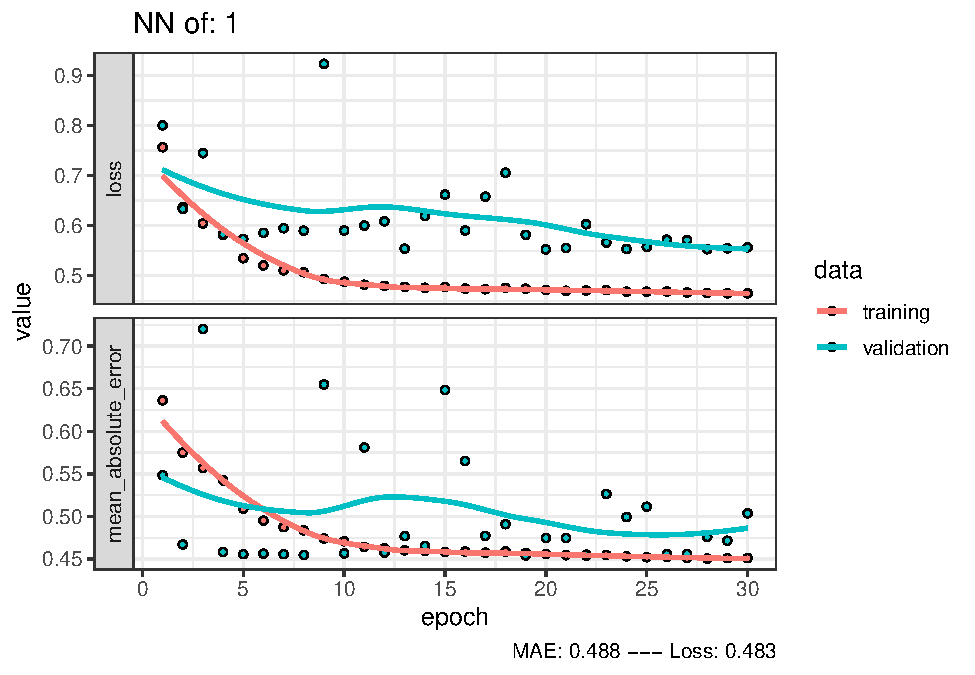
\includegraphics{project-code_files/figure-latex/unnamed-chunk-18-1.pdf}

\begin{verbatim}
## `geom_smooth()` using formula 'y ~ x'
\end{verbatim}

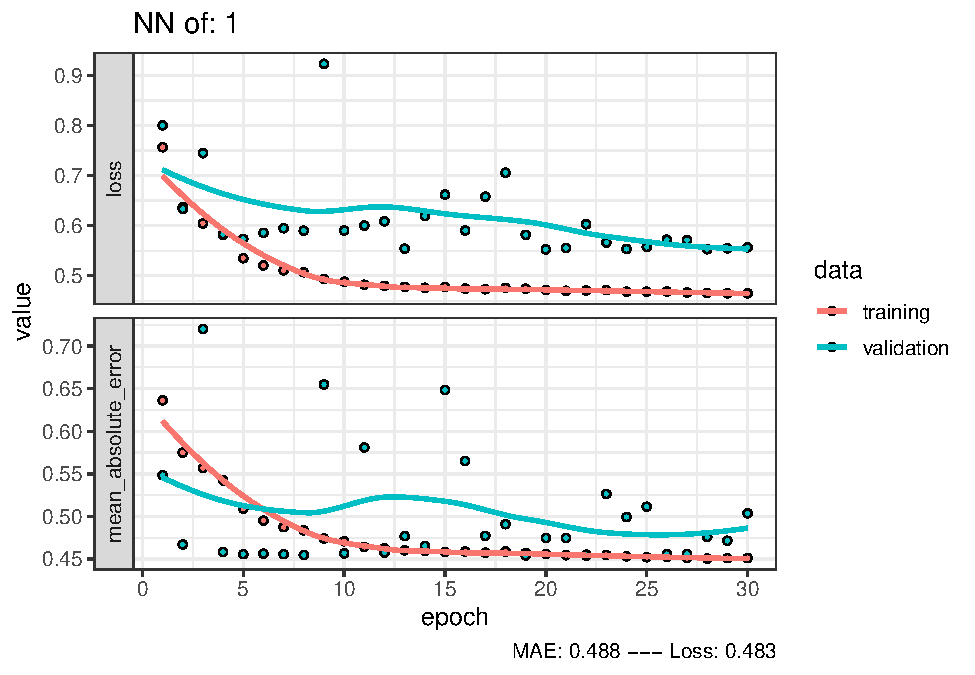
\includegraphics{project-code_files/figure-latex/unnamed-chunk-18-2.pdf}

\begin{verbatim}
## MAE:  0.4877132
## Loss:  0.4832867 
## 
## [1] "========== 2 =========="
\end{verbatim}

\begin{verbatim}
## `geom_smooth()` using formula 'y ~ x'
\end{verbatim}

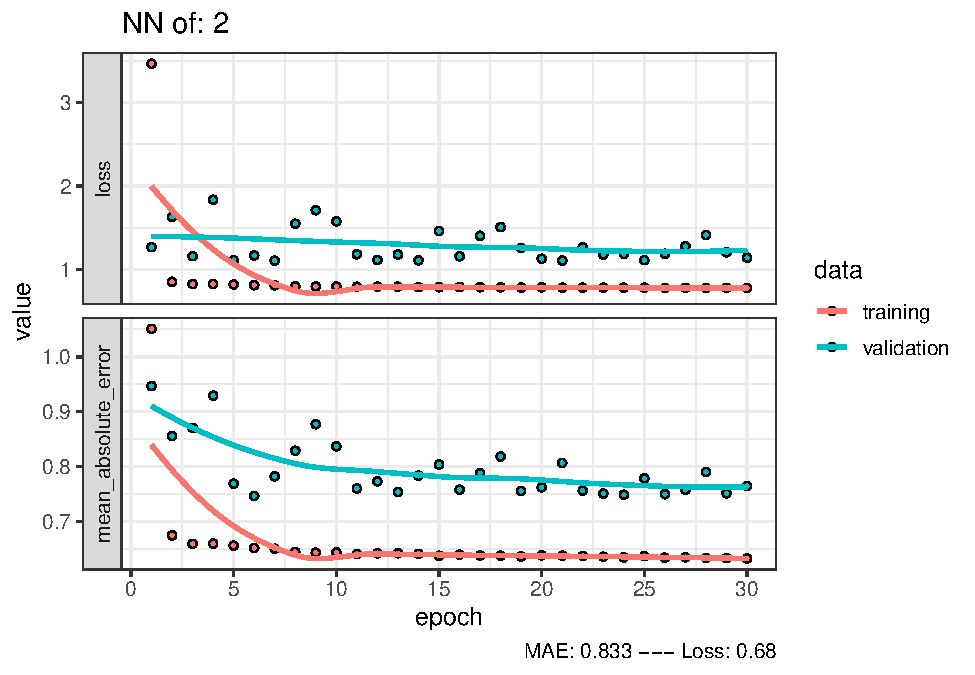
\includegraphics{project-code_files/figure-latex/unnamed-chunk-18-3.pdf}

\begin{verbatim}
## `geom_smooth()` using formula 'y ~ x'
\end{verbatim}

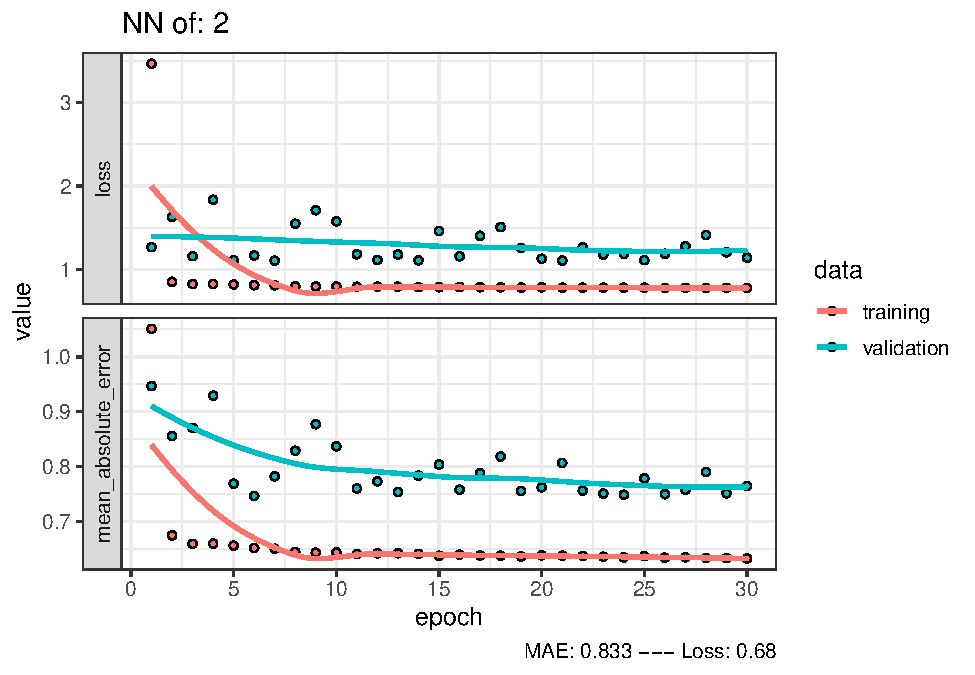
\includegraphics{project-code_files/figure-latex/unnamed-chunk-18-4.pdf}

\begin{verbatim}
## MAE:  0.8333294
## Loss:  0.6800426 
## 
## [1] "========== 3 =========="
\end{verbatim}

\begin{verbatim}
## `geom_smooth()` using formula 'y ~ x'
\end{verbatim}

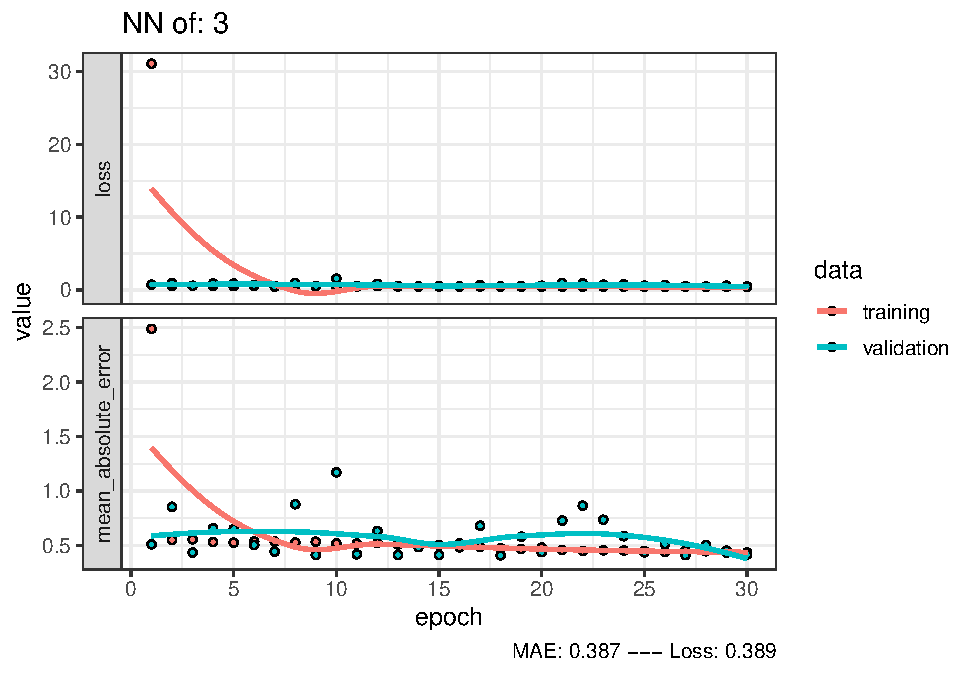
\includegraphics{project-code_files/figure-latex/unnamed-chunk-18-5.pdf}

\begin{verbatim}
## `geom_smooth()` using formula 'y ~ x'
\end{verbatim}

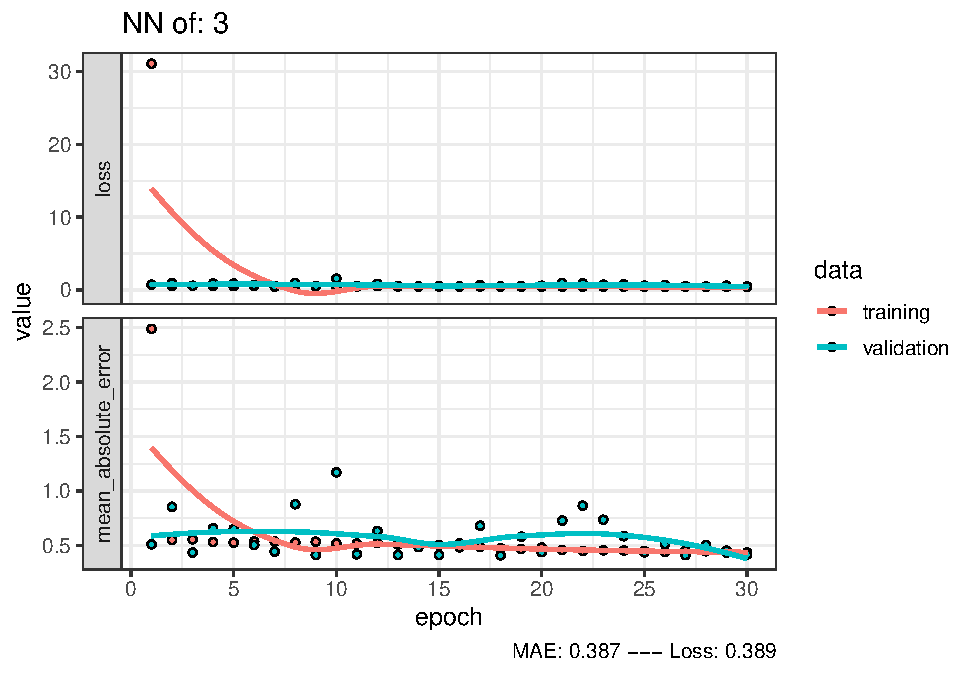
\includegraphics{project-code_files/figure-latex/unnamed-chunk-18-6.pdf}

\begin{verbatim}
## MAE:  0.3867755
## Loss:  0.3894443 
## 
## [1] "========== 4 =========="
\end{verbatim}

\begin{verbatim}
## `geom_smooth()` using formula 'y ~ x'
\end{verbatim}

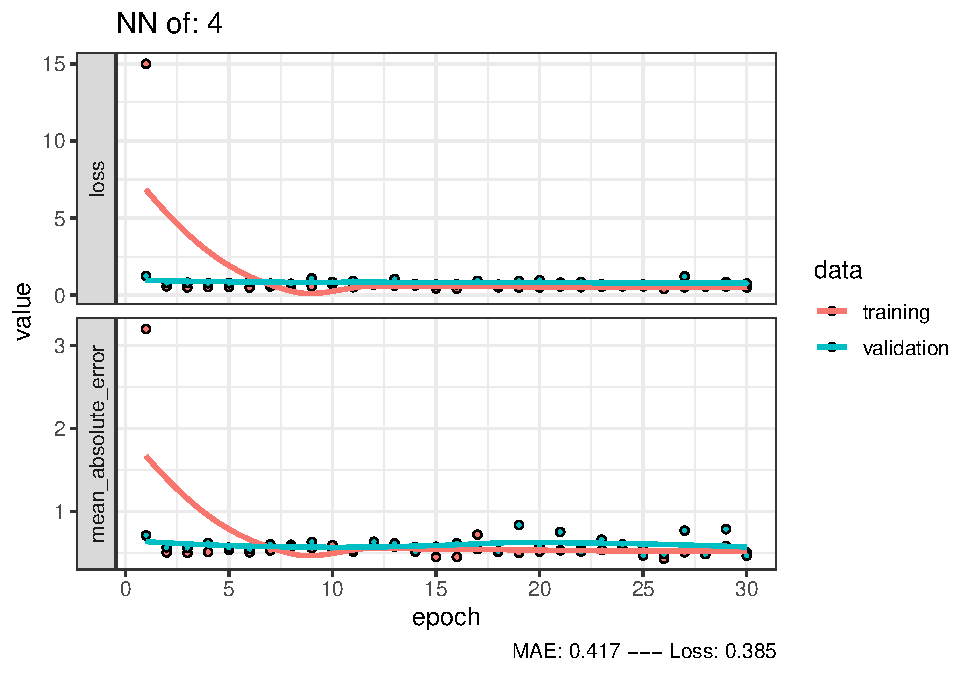
\includegraphics{project-code_files/figure-latex/unnamed-chunk-18-7.pdf}

\begin{verbatim}
## `geom_smooth()` using formula 'y ~ x'
\end{verbatim}

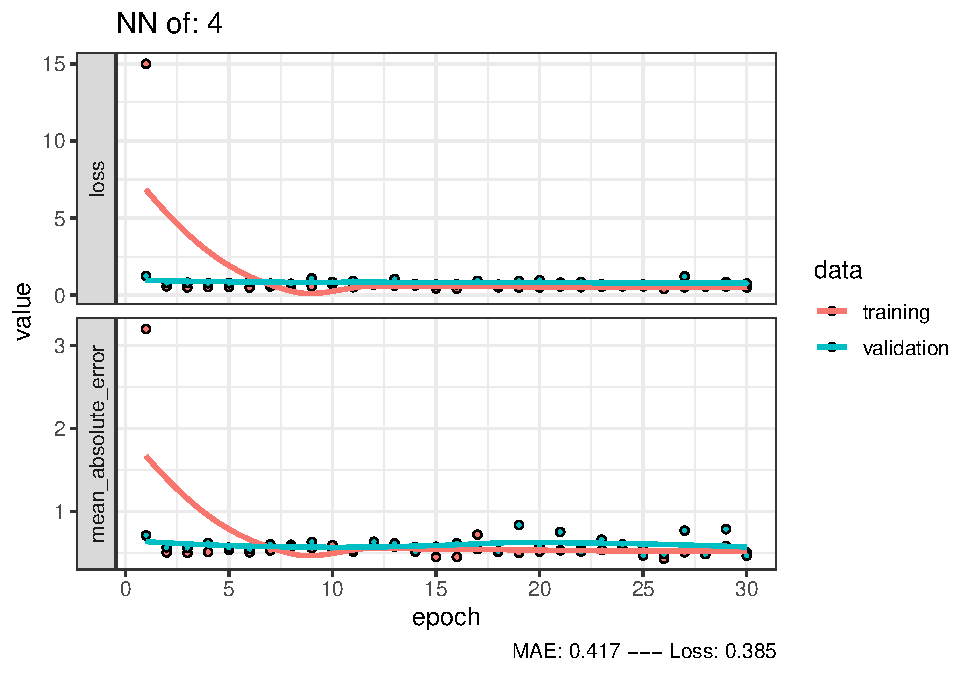
\includegraphics{project-code_files/figure-latex/unnamed-chunk-18-8.pdf}

\begin{verbatim}
## MAE:  0.417328
## Loss:  0.3846916 
## 
## [1] "========== 5 =========="
\end{verbatim}

\begin{verbatim}
## `geom_smooth()` using formula 'y ~ x'
\end{verbatim}

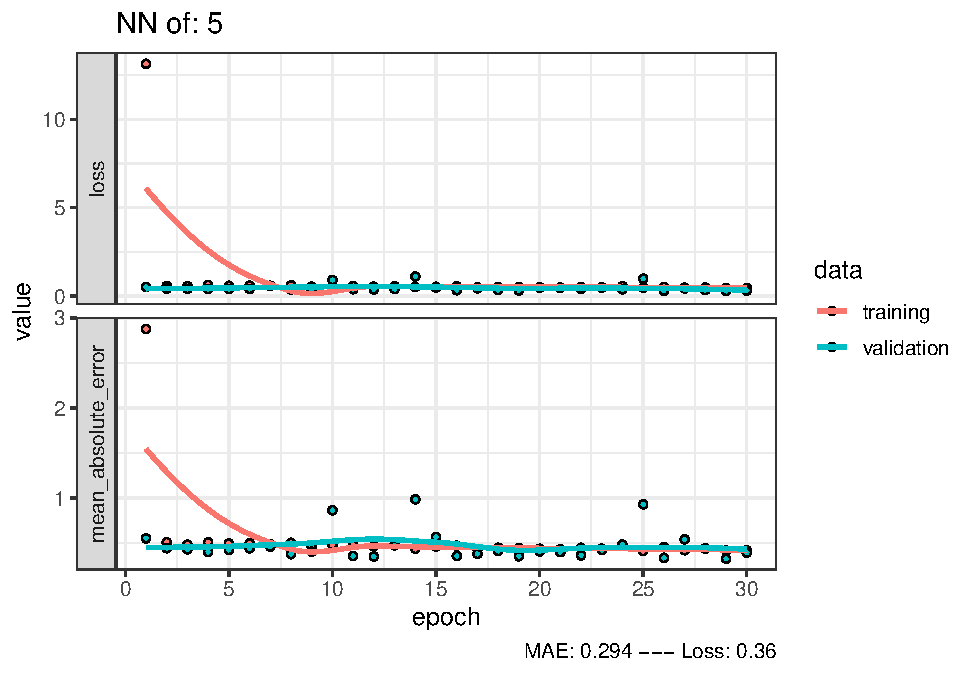
\includegraphics{project-code_files/figure-latex/unnamed-chunk-18-9.pdf}

\begin{verbatim}
## `geom_smooth()` using formula 'y ~ x'
\end{verbatim}

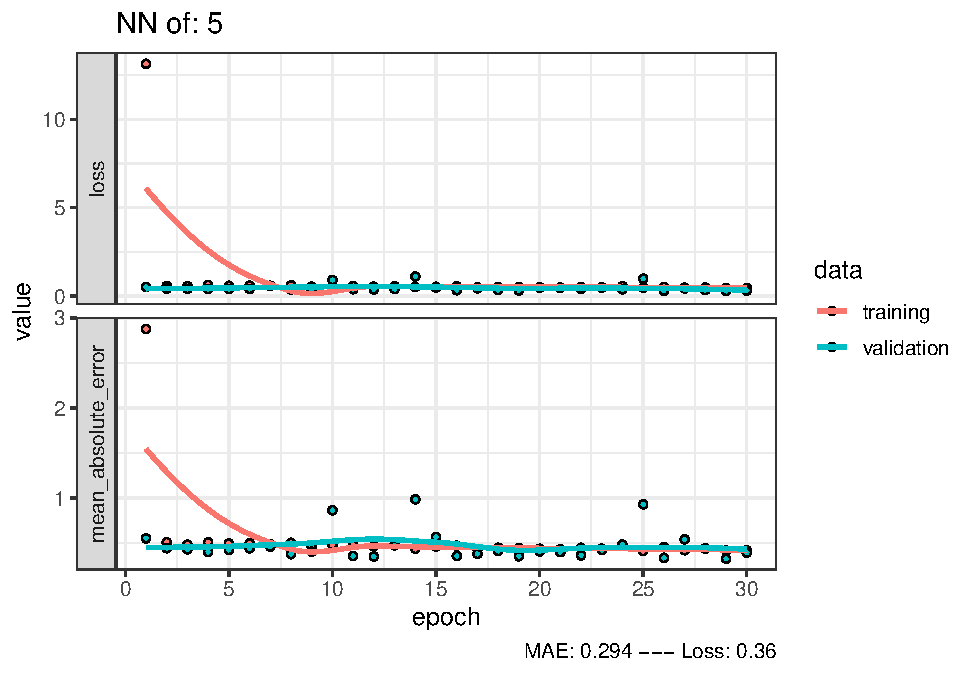
\includegraphics{project-code_files/figure-latex/unnamed-chunk-18-10.pdf}

\begin{verbatim}
## MAE:  0.2938451
## Loss:  0.359958 
## 
## [1] "========== n1-r1 =========="
\end{verbatim}

\begin{verbatim}
## `geom_smooth()` using formula 'y ~ x'
\end{verbatim}

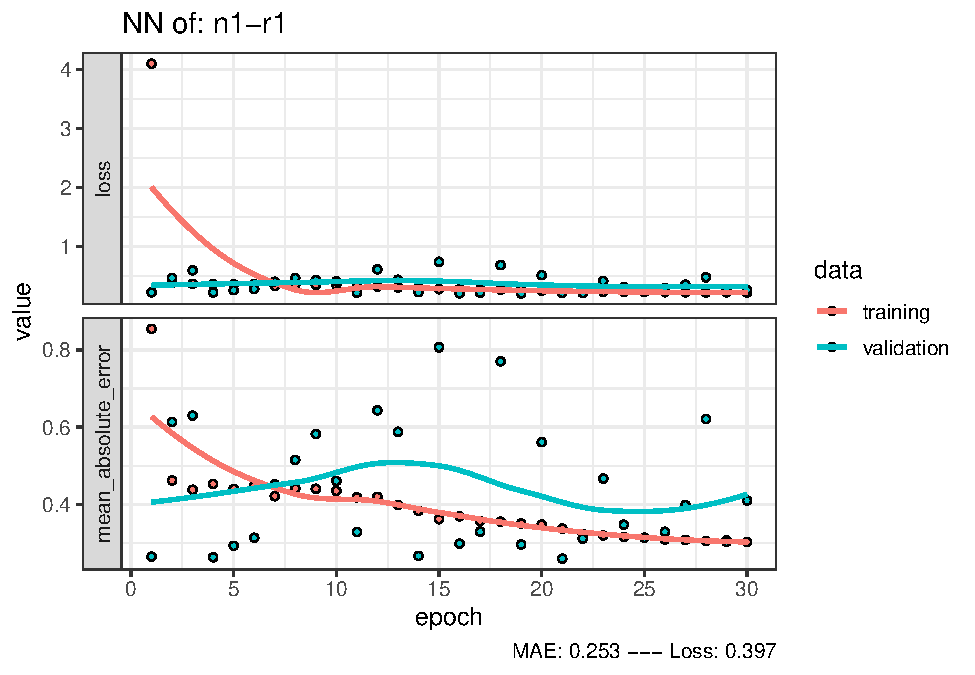
\includegraphics{project-code_files/figure-latex/unnamed-chunk-18-11.pdf}

\begin{verbatim}
## `geom_smooth()` using formula 'y ~ x'
\end{verbatim}

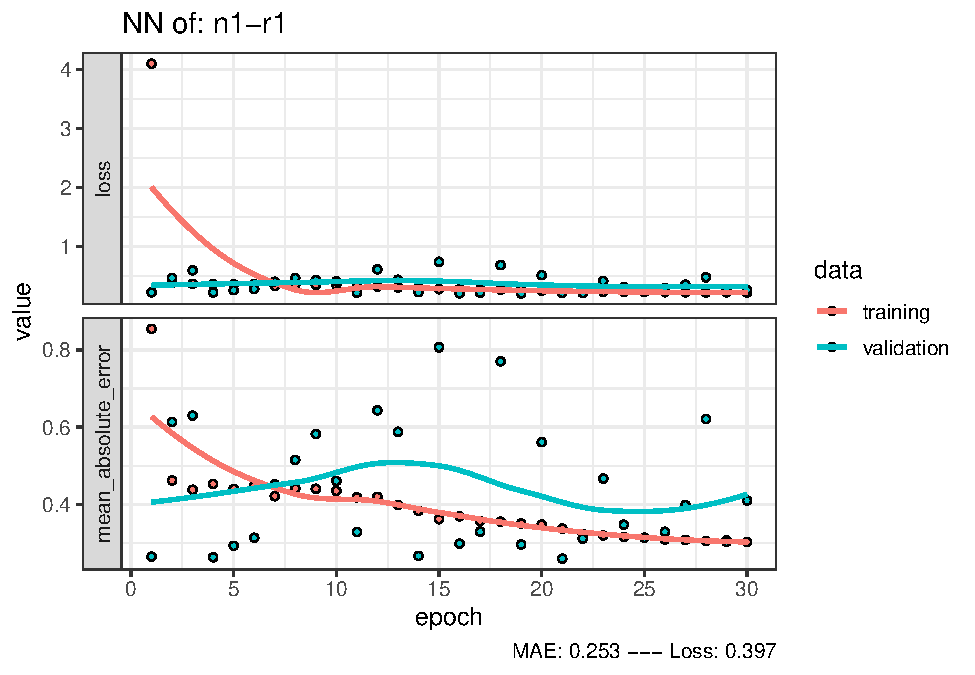
\includegraphics{project-code_files/figure-latex/unnamed-chunk-18-12.pdf}

\begin{verbatim}
## MAE:  0.252656
## Loss:  0.3968593 
## 
## [1] "========== n1-r2 =========="
\end{verbatim}

\begin{verbatim}
## `geom_smooth()` using formula 'y ~ x'
\end{verbatim}

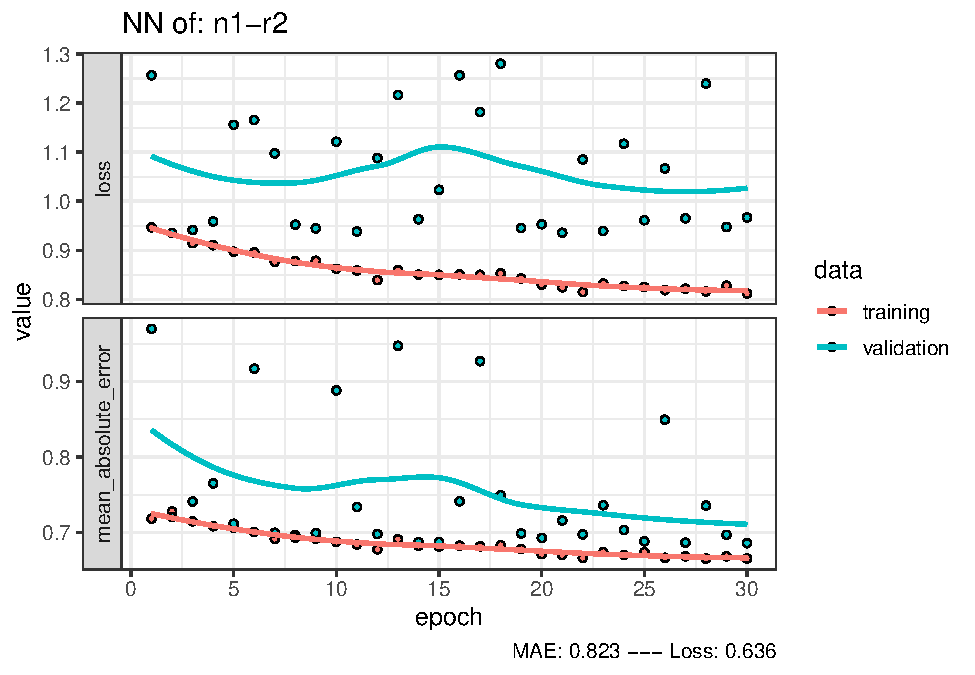
\includegraphics{project-code_files/figure-latex/unnamed-chunk-18-13.pdf}

\begin{verbatim}
## `geom_smooth()` using formula 'y ~ x'
\end{verbatim}

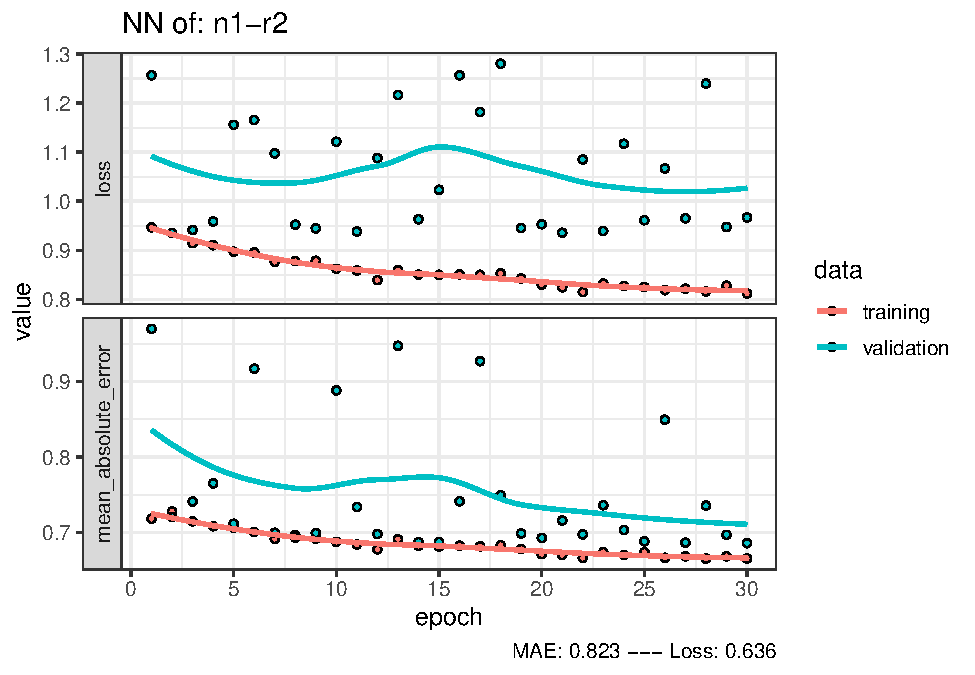
\includegraphics{project-code_files/figure-latex/unnamed-chunk-18-14.pdf}

\begin{verbatim}
## MAE:  0.823441
## Loss:  0.6362852 
## 
## [1] "========== n1-r3 =========="
\end{verbatim}

\begin{verbatim}
## `geom_smooth()` using formula 'y ~ x'
\end{verbatim}

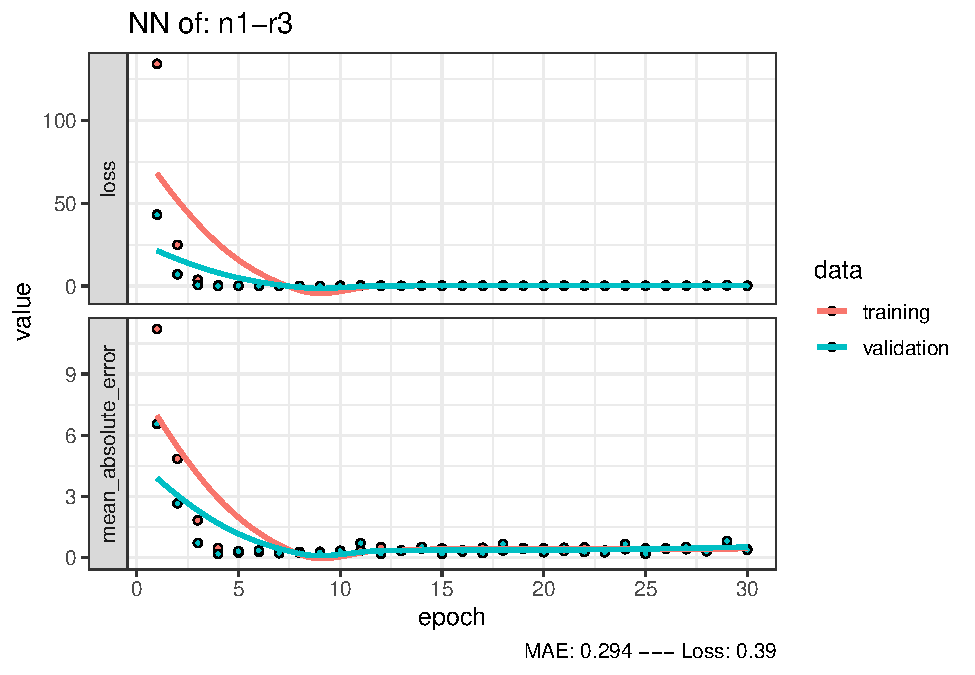
\includegraphics{project-code_files/figure-latex/unnamed-chunk-18-15.pdf}

\begin{verbatim}
## `geom_smooth()` using formula 'y ~ x'
\end{verbatim}

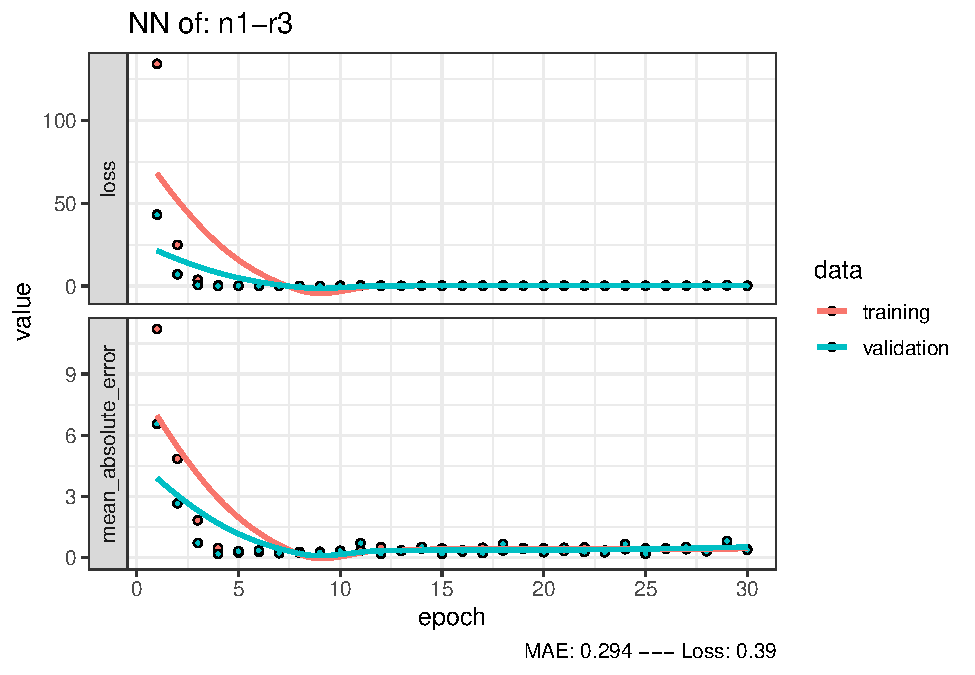
\includegraphics{project-code_files/figure-latex/unnamed-chunk-18-16.pdf}

\begin{verbatim}
## MAE:  0.2944945
## Loss:  0.389903 
## 
## [1] "========== n2-r1 =========="
\end{verbatim}

\begin{verbatim}
## `geom_smooth()` using formula 'y ~ x'
\end{verbatim}

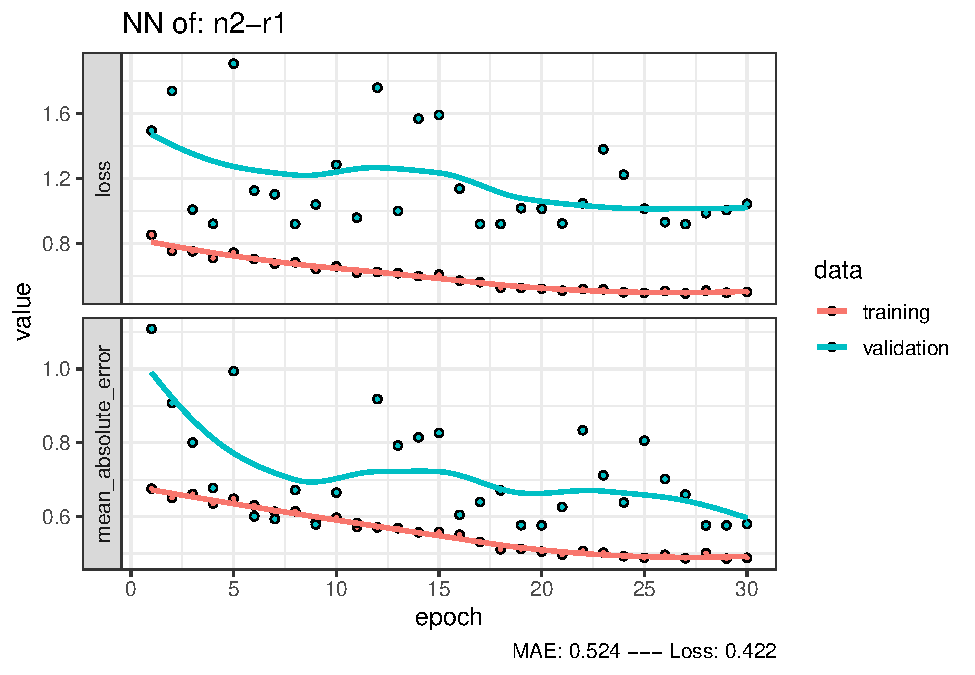
\includegraphics{project-code_files/figure-latex/unnamed-chunk-18-17.pdf}

\begin{verbatim}
## `geom_smooth()` using formula 'y ~ x'
\end{verbatim}

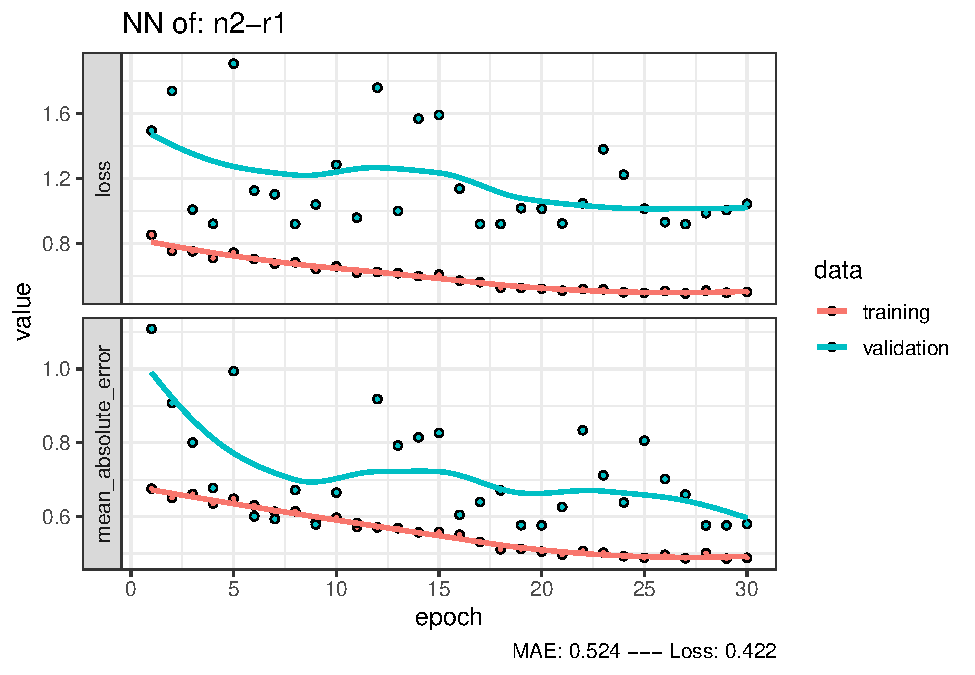
\includegraphics{project-code_files/figure-latex/unnamed-chunk-18-18.pdf}

\begin{verbatim}
## MAE:  0.5244784
## Loss:  0.4219968 
## 
## [1] "========== n2-r2 =========="
\end{verbatim}

\begin{verbatim}
## `geom_smooth()` using formula 'y ~ x'
\end{verbatim}

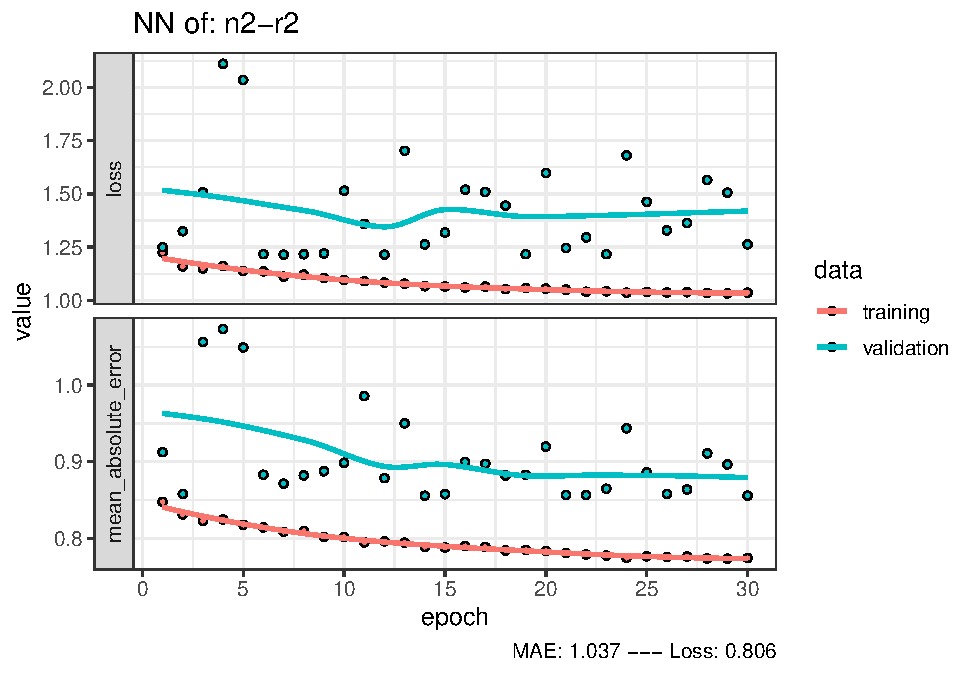
\includegraphics{project-code_files/figure-latex/unnamed-chunk-18-19.pdf}

\begin{verbatim}
## `geom_smooth()` using formula 'y ~ x'
\end{verbatim}

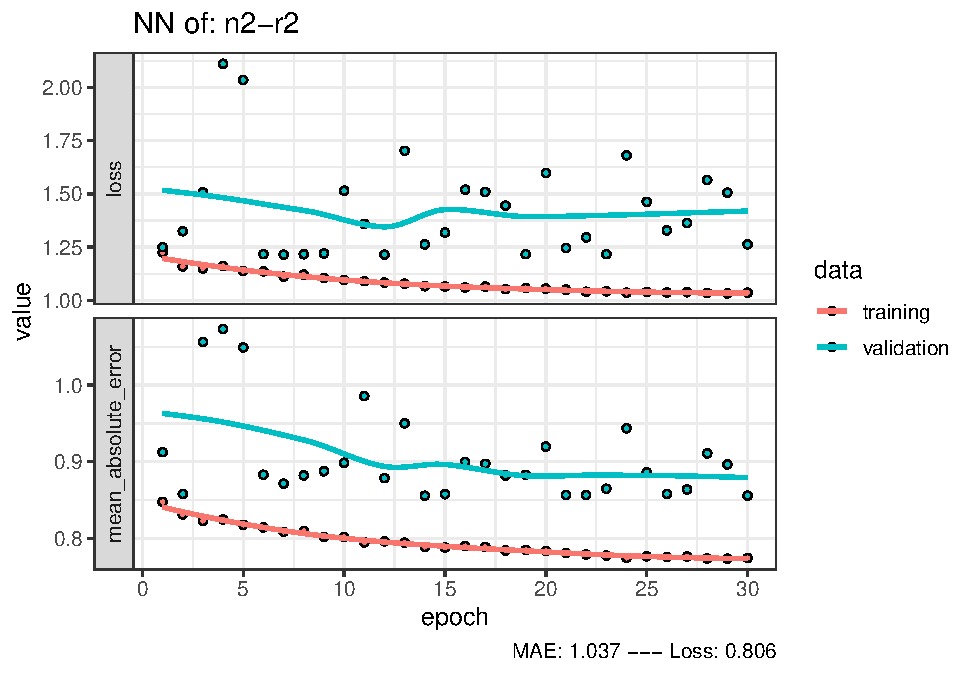
\includegraphics{project-code_files/figure-latex/unnamed-chunk-18-20.pdf}

\begin{verbatim}
## MAE:  1.037113
## Loss:  0.8063703 
## 
## [1] "========== n2-r3 =========="
\end{verbatim}

\begin{verbatim}
## `geom_smooth()` using formula 'y ~ x'
\end{verbatim}

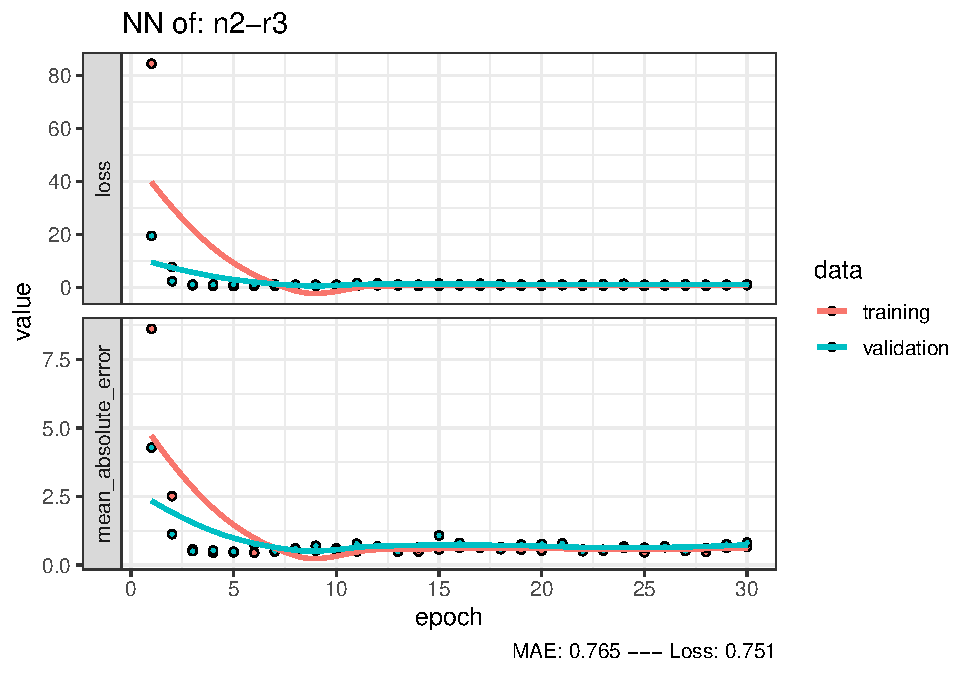
\includegraphics{project-code_files/figure-latex/unnamed-chunk-18-21.pdf}

\begin{verbatim}
## `geom_smooth()` using formula 'y ~ x'
\end{verbatim}

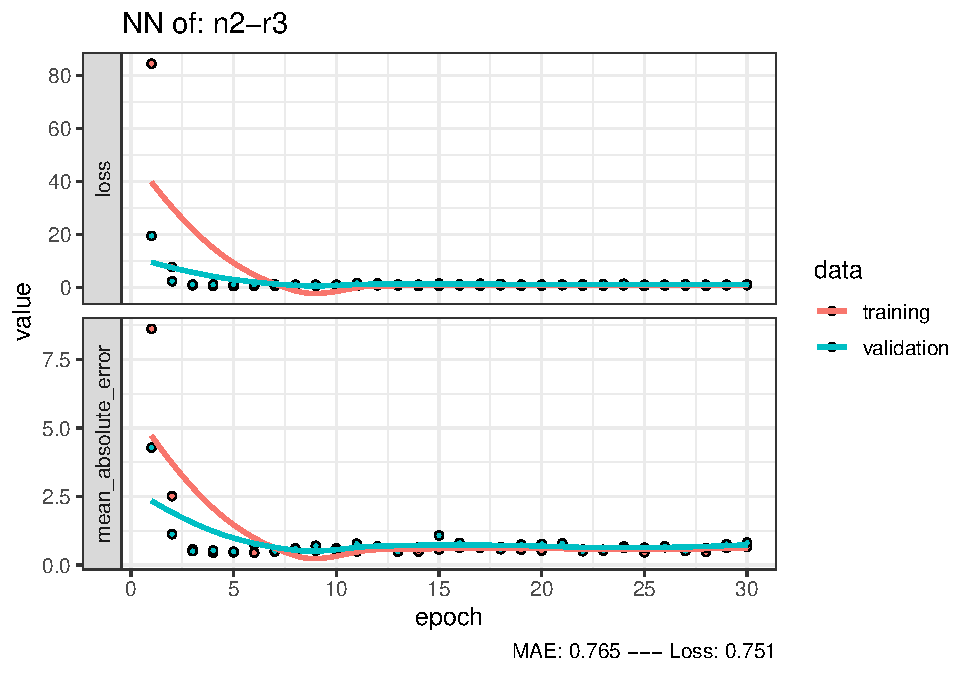
\includegraphics{project-code_files/figure-latex/unnamed-chunk-18-22.pdf}

\begin{verbatim}
## MAE:  0.7650962
## Loss:  0.750608 
## 
## [1] "========== n3-r1 =========="
\end{verbatim}

\begin{verbatim}
## `geom_smooth()` using formula 'y ~ x'
\end{verbatim}

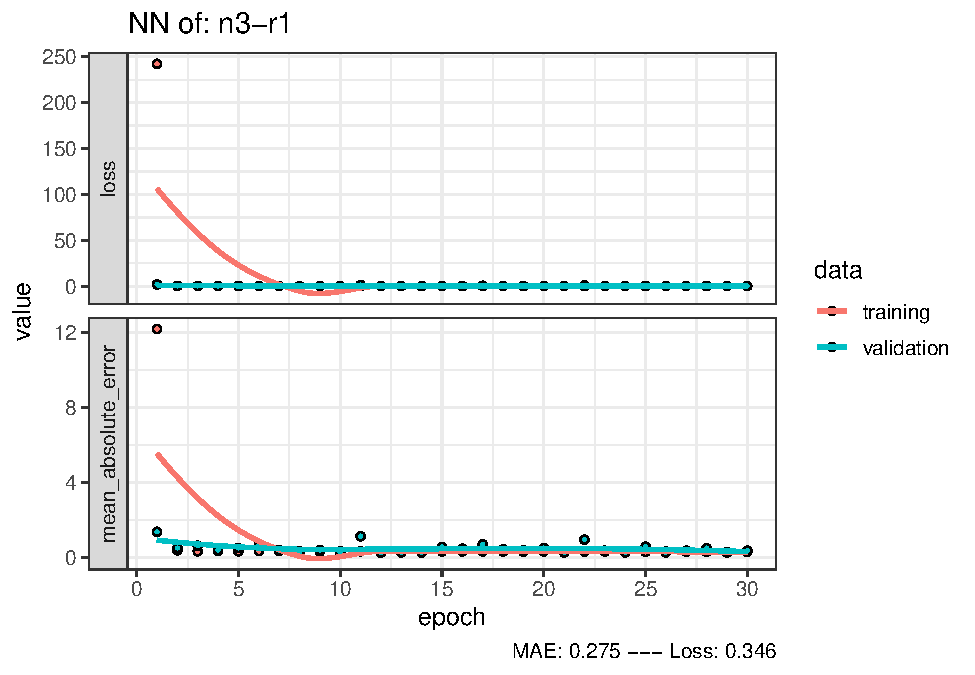
\includegraphics{project-code_files/figure-latex/unnamed-chunk-18-23.pdf}

\begin{verbatim}
## `geom_smooth()` using formula 'y ~ x'
\end{verbatim}

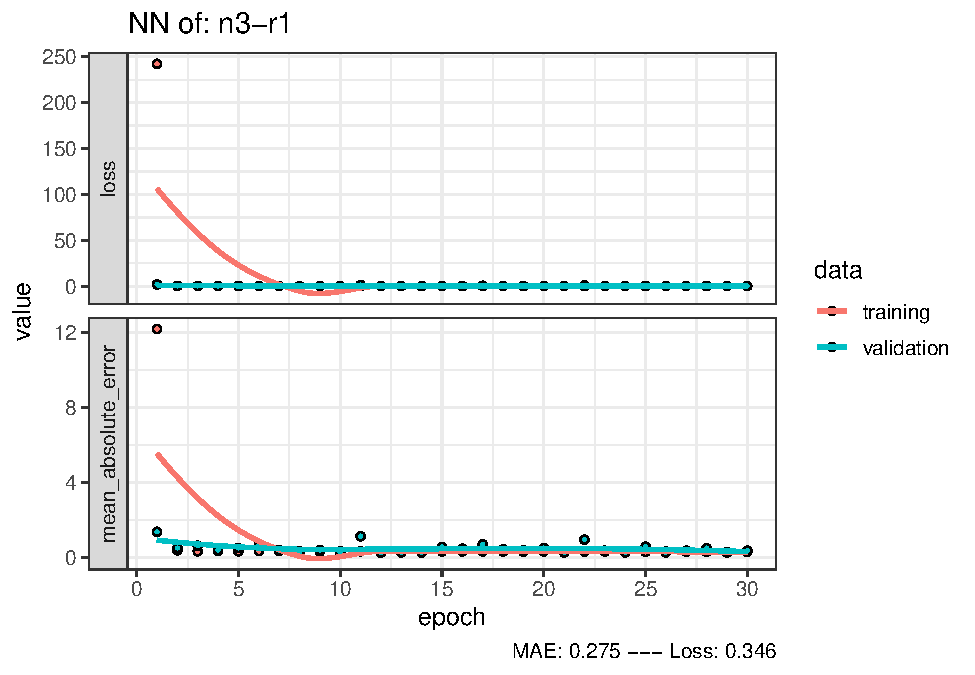
\includegraphics{project-code_files/figure-latex/unnamed-chunk-18-24.pdf}

\begin{verbatim}
## MAE:  0.2753657
## Loss:  0.3455145 
## 
## [1] "========== n3-r2 =========="
\end{verbatim}

\begin{verbatim}
## `geom_smooth()` using formula 'y ~ x'
\end{verbatim}

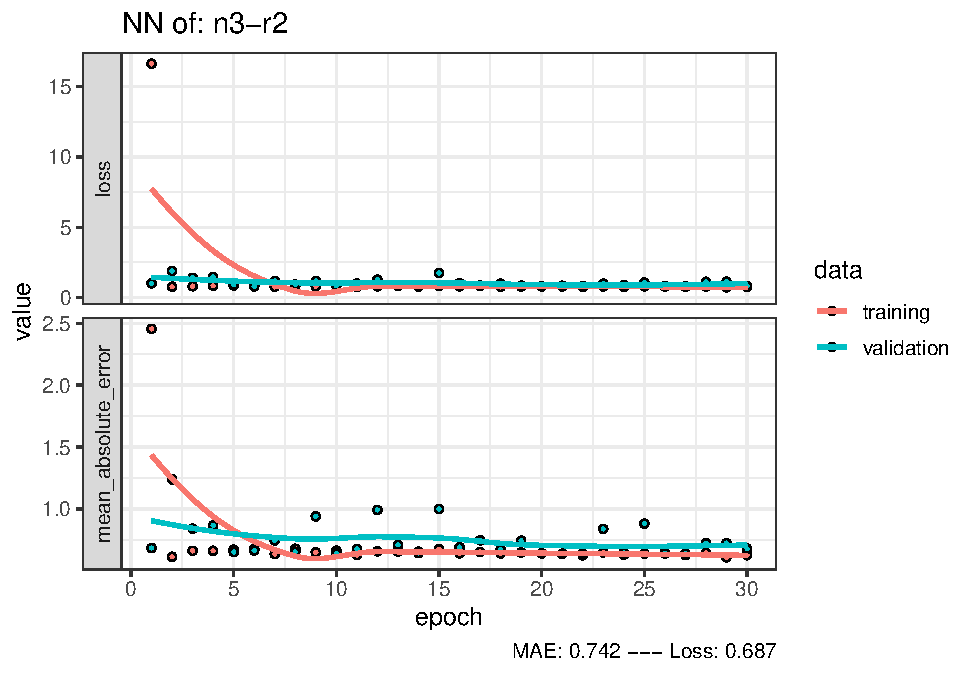
\includegraphics{project-code_files/figure-latex/unnamed-chunk-18-25.pdf}

\begin{verbatim}
## `geom_smooth()` using formula 'y ~ x'
\end{verbatim}

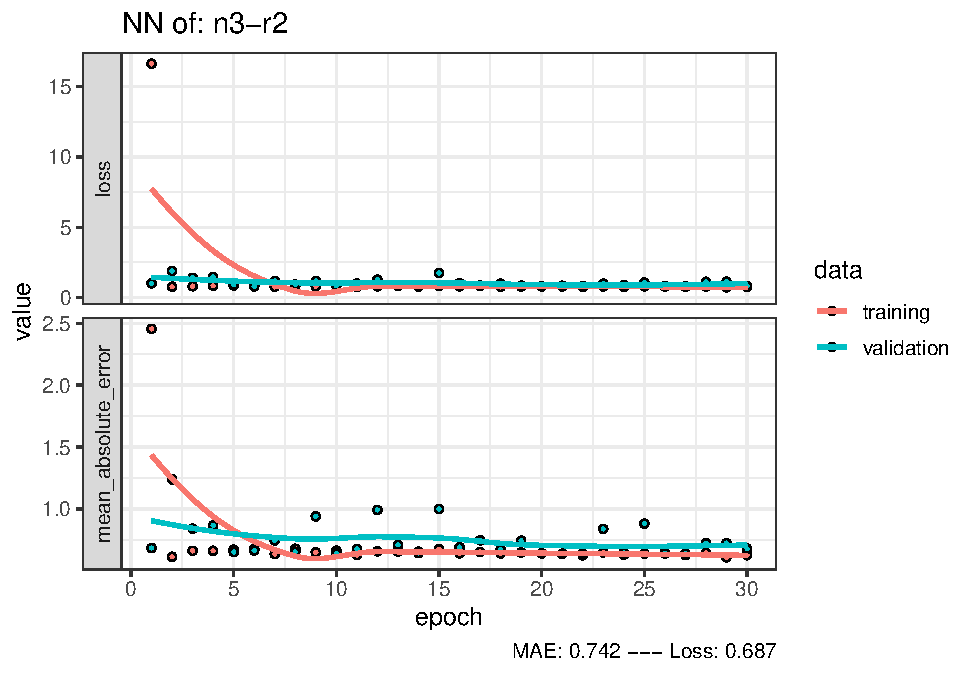
\includegraphics{project-code_files/figure-latex/unnamed-chunk-18-26.pdf}

\begin{verbatim}
## MAE:  0.7421407
## Loss:  0.686858 
## 
## [1] "========== n3-r3 =========="
\end{verbatim}

\begin{verbatim}
## `geom_smooth()` using formula 'y ~ x'
\end{verbatim}

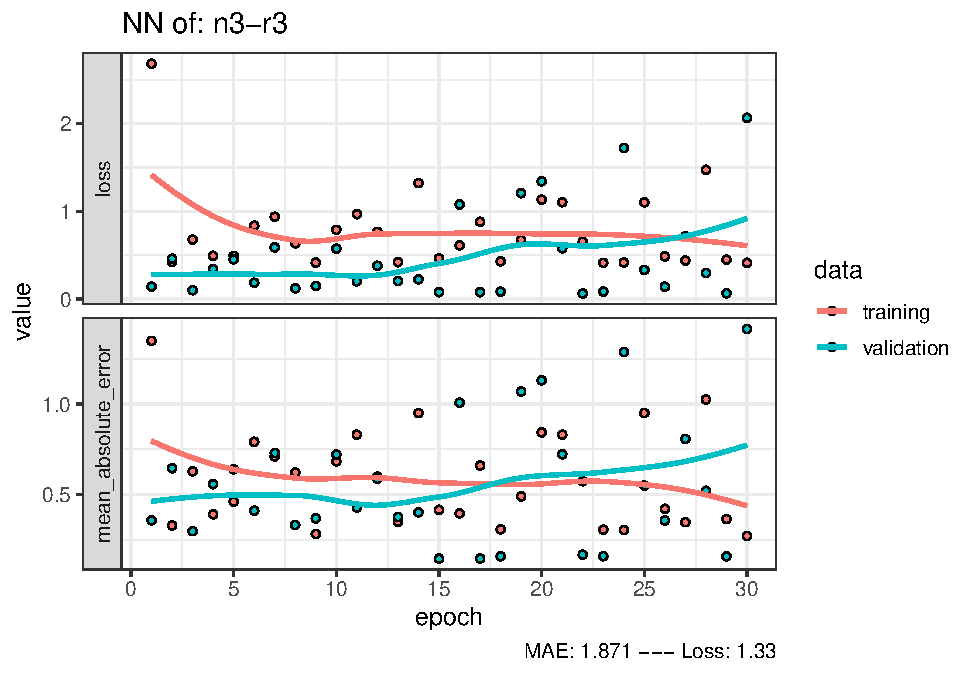
\includegraphics{project-code_files/figure-latex/unnamed-chunk-18-27.pdf}

\begin{verbatim}
## `geom_smooth()` using formula 'y ~ x'
\end{verbatim}

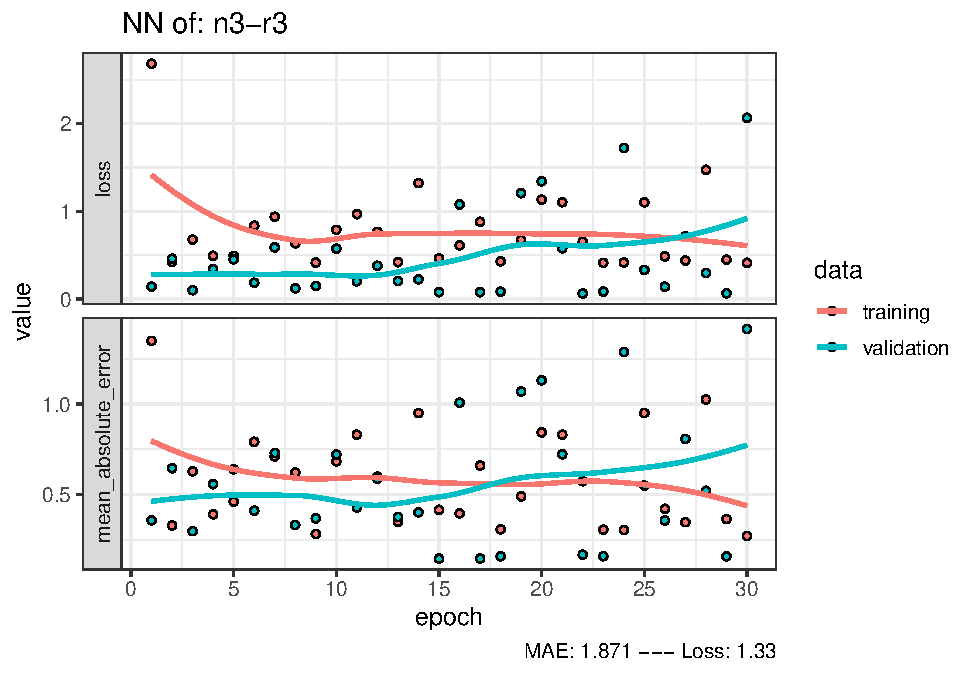
\includegraphics{project-code_files/figure-latex/unnamed-chunk-18-28.pdf}

\begin{verbatim}
## MAE:  1.87118
## Loss:  1.32991 
## 
## [1] "========== n4-r1 =========="
\end{verbatim}

\begin{verbatim}
## `geom_smooth()` using formula 'y ~ x'
\end{verbatim}

\includegraphics{project-code_files/figure-latex/unnamed-chunk-18-29.pdf}

\begin{verbatim}
## `geom_smooth()` using formula 'y ~ x'
\end{verbatim}

\includegraphics{project-code_files/figure-latex/unnamed-chunk-18-30.pdf}

\begin{verbatim}
## MAE:  0.1332488
## Loss:  0.2908146 
## 
## [1] "========== n4-r2 =========="
\end{verbatim}

\begin{verbatim}
## `geom_smooth()` using formula 'y ~ x'
\end{verbatim}

\includegraphics{project-code_files/figure-latex/unnamed-chunk-18-31.pdf}

\begin{verbatim}
## `geom_smooth()` using formula 'y ~ x'
\end{verbatim}

\includegraphics{project-code_files/figure-latex/unnamed-chunk-18-32.pdf}

\begin{verbatim}
## MAE:  0.6004597
## Loss:  0.555418 
## 
## [1] "========== n4-r3 =========="
\end{verbatim}

\begin{verbatim}
## `geom_smooth()` using formula 'y ~ x'
\end{verbatim}

\includegraphics{project-code_files/figure-latex/unnamed-chunk-18-33.pdf}

\begin{verbatim}
## `geom_smooth()` using formula 'y ~ x'
\end{verbatim}

\includegraphics{project-code_files/figure-latex/unnamed-chunk-18-34.pdf}

\begin{verbatim}
## MAE:  0.5377738
## Loss:  0.6261361 
## 
## [1] "========== n5-r1 =========="
\end{verbatim}

\begin{verbatim}
## `geom_smooth()` using formula 'y ~ x'
\end{verbatim}

\includegraphics{project-code_files/figure-latex/unnamed-chunk-18-35.pdf}

\begin{verbatim}
## `geom_smooth()` using formula 'y ~ x'
\end{verbatim}

\includegraphics{project-code_files/figure-latex/unnamed-chunk-18-36.pdf}

\begin{verbatim}
## MAE:  0.5982274
## Loss:  0.6743885 
## 
## [1] "========== n5-r2 =========="
\end{verbatim}

\begin{verbatim}
## `geom_smooth()` using formula 'y ~ x'
\end{verbatim}

\includegraphics{project-code_files/figure-latex/unnamed-chunk-18-37.pdf}

\begin{verbatim}
## `geom_smooth()` using formula 'y ~ x'
\end{verbatim}

\includegraphics{project-code_files/figure-latex/unnamed-chunk-18-38.pdf}

\begin{verbatim}
## MAE:  0.9505594
## Loss:  0.7829418 
## 
## [1] "========== n5-r3 =========="
\end{verbatim}

\begin{verbatim}
## `geom_smooth()` using formula 'y ~ x'
\end{verbatim}

\includegraphics{project-code_files/figure-latex/unnamed-chunk-18-39.pdf}

\begin{verbatim}
## `geom_smooth()` using formula 'y ~ x'
\end{verbatim}

\includegraphics{project-code_files/figure-latex/unnamed-chunk-18-40.pdf}

\begin{verbatim}
## MAE:  0.1779435
## Loss:  0.2803045 
## 
## [1] "========== all =========="
\end{verbatim}

\begin{verbatim}
## `geom_smooth()` using formula 'y ~ x'
\end{verbatim}

\includegraphics{project-code_files/figure-latex/unnamed-chunk-18-41.pdf}

\begin{verbatim}
## `geom_smooth()` using formula 'y ~ x'
\end{verbatim}

\includegraphics{project-code_files/figure-latex/unnamed-chunk-18-42.pdf}

\begin{verbatim}
## MAE:  0.6347676
## Loss:  0.5417054
\end{verbatim}

~\\

\hypertarget{comparison-between-the-models}{%
\section{Comparison between the
models}\label{comparison-between-the-models}}

~\\

\begin{Shaded}
\begin{Highlighting}[]
\NormalTok{conc =}\StringTok{ }\KeywordTok{c}\NormalTok{()}

\ControlFlowTok{for}\NormalTok{ (n }\ControlFlowTok{in} \KeywordTok{unique}\NormalTok{(ds}\OperatorTok{$}\NormalTok{neighbourhood_group))}
\NormalTok{\{}
\NormalTok{  conc =}\StringTok{ }\KeywordTok{c}\NormalTok{(conc,n) }
\NormalTok{\}}
\ControlFlowTok{for}\NormalTok{ (n }\ControlFlowTok{in} \KeywordTok{unique}\NormalTok{(ds}\OperatorTok{$}\NormalTok{neighbourhood_group))}
\NormalTok{\{}
  \ControlFlowTok{for}\NormalTok{(r }\ControlFlowTok{in} \KeywordTok{unique}\NormalTok{(ds}\OperatorTok{$}\NormalTok{room_type))}
\NormalTok{  \{}
\NormalTok{    conc =}\StringTok{ }\KeywordTok{c}\NormalTok{(conc, }\KeywordTok{paste}\NormalTok{(n,}\StringTok{"-"}\NormalTok{,r))}
    
\NormalTok{  \}}
\NormalTok{\}}
\NormalTok{conc =}\StringTok{ }\KeywordTok{c}\NormalTok{(conc,}\StringTok{"All"}\NormalTok{)}

\NormalTok{n =}\StringTok{ }\KeywordTok{names}\NormalTok{(nn)}



\NormalTok{cols =}\StringTok{ }\KeywordTok{vector}\NormalTok{(}\StringTok{"list"}\NormalTok{)}
\NormalTok{cols[[}\StringTok{"Subset"}\NormalTok{]] =}\StringTok{ }\NormalTok{conc}
\ControlFlowTok{for}\NormalTok{( m }\ControlFlowTok{in}\NormalTok{ model_lis)}
\NormalTok{\{}
\NormalTok{  col =}\StringTok{ }\KeywordTok{c}\NormalTok{()}
  \ControlFlowTok{for}\NormalTok{( nam }\ControlFlowTok{in}\NormalTok{ n)}
\NormalTok{  \{}
    
    \ControlFlowTok{if}\NormalTok{( nam }\OperatorTok{!=}\StringTok{ "name"}\NormalTok{)}
\NormalTok{    \{ }
\NormalTok{      col =}\StringTok{ }\KeywordTok{c}\NormalTok{(col,m[[nam]]}\OperatorTok{$}\NormalTok{MSE)  }
      
\NormalTok{    \}}
    
\NormalTok{  \}}
\NormalTok{  cols[[m}\OperatorTok{$}\NormalTok{name]] =}\StringTok{ }\NormalTok{col}
  
\NormalTok{\}}


\NormalTok{mse_df =}\StringTok{ }\KeywordTok{as.data.frame}\NormalTok{(cols)}
\NormalTok{best =}\StringTok{ }\KeywordTok{c}\NormalTok{()}
\ControlFlowTok{for}\NormalTok{ (i }\ControlFlowTok{in} \DecValTok{1}\OperatorTok{:}\KeywordTok{length}\NormalTok{(cols}\OperatorTok{$}\NormalTok{Subset))}
\NormalTok{\{}
\NormalTok{  m =}\StringTok{ }\KeywordTok{min}\NormalTok{(mse_df[i,}\DecValTok{2}\OperatorTok{:}\DecValTok{6}\NormalTok{])}
\NormalTok{  col =}\StringTok{ }\KeywordTok{which}\NormalTok{(mse_df[i,}\DecValTok{1}\OperatorTok{:}\DecValTok{6}\NormalTok{ ] }\OperatorTok{==}\StringTok{ }\NormalTok{m)}
\NormalTok{  nam =}\StringTok{ }\KeywordTok{names}\NormalTok{(mse_df)[col]}
\NormalTok{  best =}\StringTok{ }\KeywordTok{c}\NormalTok{(best, nam)}
\NormalTok{\}}
\NormalTok{mse_df}\OperatorTok{$}\NormalTok{Best =}\StringTok{ }\NormalTok{best}
\CommentTok{#kableExtra::kable(mse_df)%>%}
\CommentTok{#  kable_styling(bootstrap_options = "striped", full_width = F,font_size = 20) %>%}
\CommentTok{##  row_spec(0, bold = T, color = "white", background = "#D7261E")%>%}
\CommentTok{##  column_spec(1, bold = T, border_right = T,color = "white", background = "#191970")%>%}
\CommentTok{#  column_spec(2:6,extra_css="text-align:Center")}

\NormalTok{mse_df}
\end{Highlighting}
\end{Shaded}

\begin{verbatim}
##                             Subset Linear.Regression Decision.Tree
## 1                         Brooklyn         0.4581633     0.4607817
## 2                        Manhattan         0.7581404     0.7634093
## 3                           Queens         0.3846665     0.3864543
## 4                    Staten Island         0.3467308     0.3471879
## 5                            Bronx         0.2741482     0.2744778
## 6          Brooklyn - Private room         0.1818182     0.1771088
## 7       Brooklyn - Entire home/apt         0.7598732     0.7503308
## 8           Brooklyn - Shared room         0.2639579     0.2505339
## 9         Manhattan - Private room         0.4445611     0.3753113
## 10     Manhattan - Entire home/apt         0.9361941     0.9585893
## 11         Manhattan - Shared room         0.4904792     0.4992158
## 12           Queens - Private room         0.1616290     0.1551588
## 13        Queens - Entire home/apt         0.6992986     0.6995247
## 14            Queens - Shared room         0.1659605     0.1667691
## 15    Staten Island - Private room         0.1332495     0.1605553
## 16 Staten Island - Entire home/apt         0.5703345     0.7737648
## 17     Staten Island - Shared room         0.3209208     0.5818964
## 18            Bronx - Private room         0.1475827     0.1611146
## 19         Bronx - Entire home/apt         0.8252451     0.8860040
## 20             Bronx - Shared room         0.2071295     0.1939584
## 21                             All         0.6167807     0.6149423
##    Random.Forest Ranger.Random.Forest Neural.Networks                 Best
## 1      0.4376492            0.4356612       0.4877132 Ranger.Random.Forest
## 2      0.7150546            0.7132323       0.8333294 Ranger.Random.Forest
## 3      0.3601118            0.3594399       0.3867755 Ranger.Random.Forest
## 4      0.3433679            0.3498251       0.4173280        Random.Forest
## 5      0.2714934            0.2680627       0.2938451 Ranger.Random.Forest
## 6      0.1837738            0.1830508       0.2526560        Decision.Tree
## 7      0.8019234            0.8056467       0.8234408        Decision.Tree
## 8      0.2406699            0.2386268       0.2944945 Ranger.Random.Forest
## 9      0.3784497            0.3782840       0.5244784        Decision.Tree
## 10     0.9771422            0.9743580       1.0371131    Linear.Regression
## 11     0.5635043            0.5715526       0.7650962    Linear.Regression
## 12     0.1517223            0.1527042       0.2753657        Random.Forest
## 13     0.7135788            0.7123861       0.7421406    Linear.Regression
## 14     0.2229526            0.2213944       1.8711798    Linear.Regression
## 15     0.1423578            0.1433902       0.1332488      Neural.Networks
## 16     0.7189537            0.7056397       0.6004597    Linear.Regression
## 17     0.3032279            0.5847496       0.5377738        Random.Forest
## 18     0.1330848            0.1327536       0.5982274 Ranger.Random.Forest
## 19     0.8700947            0.8708723       0.9505594    Linear.Regression
## 20     0.1763329            0.1768414       0.1779435        Random.Forest
## 21     0.5852325            0.5539925       0.6347674 Ranger.Random.Forest
\end{verbatim}

~~

~\\

\hypertarget{clustering-and-groups}{%
\section{Clustering and Groups}\label{clustering-and-groups}}

~\\

\hypertarget{clustering-for-mixed-type-of-data}{%
\subsection{Clustering for Mixed type of
data}\label{clustering-for-mixed-type-of-data}}

\begin{Shaded}
\begin{Highlighting}[]
\NormalTok{clust_num =}\StringTok{ }\DecValTok{5}

\NormalTok{get_clusters =}\StringTok{ }\ControlFlowTok{function}\NormalTok{(dts, num, dim_plot,name)}
\NormalTok{\{}
\NormalTok{  l =}\StringTok{ }\KeywordTok{list}\NormalTok{()}
  \ControlFlowTok{if}\NormalTok{(}\KeywordTok{is.null}\NormalTok{(dts}\OperatorTok{$}\NormalTok{room_type))}
\NormalTok{  \{}
\NormalTok{    l}\OperatorTok{$}\NormalTok{cl =}\StringTok{ }\KeywordTok{kmeans}\NormalTok{(dts,num)}
\NormalTok{  \}}
  \ControlFlowTok{else}
\NormalTok{  \{}
\NormalTok{    l}\OperatorTok{$}\NormalTok{cl =}\StringTok{ }\KeywordTok{kproto}\NormalTok{(dts,num)}
    
\NormalTok{  \}}
  
\NormalTok{  clust =}\StringTok{ }\KeywordTok{list}\NormalTok{()}
  
  \ControlFlowTok{for}\NormalTok{ (i }\ControlFlowTok{in} \DecValTok{1}\OperatorTok{:}\NormalTok{num)}
\NormalTok{  \{}
\NormalTok{    indexes =}\StringTok{ }\NormalTok{l}\OperatorTok{$}\NormalTok{cl}\OperatorTok{$}\NormalTok{cluster }\OperatorTok{==}\StringTok{ }\NormalTok{i}
\NormalTok{    clust[[i]] =}\StringTok{ }\NormalTok{dts[indexes,]}
\NormalTok{  \}}
  
\NormalTok{  min_lat =}\StringTok{  }\NormalTok{dim_plot[}\DecValTok{1}\NormalTok{]}
\NormalTok{  max_lat =}\StringTok{ }\NormalTok{dim_plot[}\DecValTok{2}\NormalTok{]}
\NormalTok{  min_long =}\StringTok{ }\NormalTok{dim_plot[}\DecValTok{3}\NormalTok{]}
\NormalTok{  max_long=}\StringTok{ }\NormalTok{dim_plot[}\DecValTok{4}\NormalTok{]}
  
  
\NormalTok{  myplot=}\StringTok{ }\KeywordTok{ggplot}\NormalTok{() }\OperatorTok{+}\StringTok{  }\KeywordTok{background_image}\NormalTok{(img)}\OperatorTok{+}\StringTok{  }\KeywordTok{xlab}\NormalTok{(}\StringTok{'Longitude'}\NormalTok{) }\OperatorTok{+}\StringTok{  }\KeywordTok{ylab}\NormalTok{(}\StringTok{'Latitude'}\NormalTok{)}\OperatorTok{+}\StringTok{ }\KeywordTok{theme}\NormalTok{(}\DataTypeTok{plot.margin =} \KeywordTok{unit}\NormalTok{(}\KeywordTok{c}\NormalTok{(}\DecValTok{1}\NormalTok{,}\DecValTok{1}\NormalTok{,}\DecValTok{1}\NormalTok{,}\DecValTok{1}\NormalTok{),}\StringTok{"cm"}\NormalTok{),}\DataTypeTok{legend.title =} \KeywordTok{element_text}\NormalTok{(}\DataTypeTok{colour=}\StringTok{"blue"}\NormalTok{, }\DataTypeTok{size=}\DecValTok{10}\NormalTok{, }\DataTypeTok{face=}\StringTok{"bold"}\NormalTok{)) }\OperatorTok{+}\StringTok{ }\KeywordTok{xlim}\NormalTok{(min_long, max_long) }\OperatorTok{+}\StringTok{ }\KeywordTok{ylim}\NormalTok{(min_lat,max_lat) }\OperatorTok{+}\KeywordTok{ggtitle}\NormalTok{(}\KeywordTok{paste0}\NormalTok{(}\StringTok{"Clusters of "}\NormalTok{, name  ))}
  
  
\NormalTok{  count =}\StringTok{ }\DecValTok{1}
\NormalTok{  l}\OperatorTok{$}\NormalTok{clust_plot =}\StringTok{ }\KeywordTok{vector}\NormalTok{(}\StringTok{"list"}\NormalTok{)}
  \ControlFlowTok{for}\NormalTok{(el }\ControlFlowTok{in}\NormalTok{ clust)}
\NormalTok{  \{}
\NormalTok{    myplot =}\StringTok{ }\NormalTok{myplot}\OperatorTok{+}\StringTok{ }\KeywordTok{geom_point}\NormalTok{(}\DataTypeTok{data =}\NormalTok{ el, }\KeywordTok{aes}\NormalTok{(}\DataTypeTok{y =}\NormalTok{ latitude, }\DataTypeTok{x =}\NormalTok{ longitude),}\DataTypeTok{color=}\NormalTok{ count)}
    
\NormalTok{    p =}\KeywordTok{ggplot}\NormalTok{()}\OperatorTok{+}\StringTok{ }\KeywordTok{background_image}\NormalTok{(img)}\OperatorTok{+}\KeywordTok{geom_point}\NormalTok{(}\DataTypeTok{data =}\NormalTok{ el, }\KeywordTok{aes}\NormalTok{(}\DataTypeTok{y =}\NormalTok{ latitude, }\DataTypeTok{x =}\NormalTok{ longitude),}\DataTypeTok{color=}\NormalTok{ count) }\OperatorTok{+}\StringTok{ }\KeywordTok{xlim}\NormalTok{(min_long, max_long) }\OperatorTok{+}\StringTok{ }\KeywordTok{ylim}\NormalTok{(min_lat,max_lat) }\OperatorTok{+}\StringTok{ }\KeywordTok{ggtitle}\NormalTok{(}\KeywordTok{paste0}\NormalTok{(}\StringTok{"Cluster: "}\NormalTok{, count,}\StringTok{" of "}\NormalTok{, name  ))}
    
\NormalTok{    l}\OperatorTok{$}\NormalTok{clust_plot[[}\KeywordTok{as.character}\NormalTok{(count)]] =}\StringTok{ }\NormalTok{p}
    
\NormalTok{    l}\OperatorTok{$}\NormalTok{summary[[}\KeywordTok{as.character}\NormalTok{(count)]] =}\StringTok{ }\KeywordTok{summary}\NormalTok{(el)}

\NormalTok{    count=}\StringTok{ }\NormalTok{count}\OperatorTok{+}\DecValTok{1}
\NormalTok{  \}}
\NormalTok{  l}\OperatorTok{$}\NormalTok{myplot =}\StringTok{ }\NormalTok{myplot}
  \KeywordTok{return}\NormalTok{(l)}
\NormalTok{\}}

\NormalTok{get_all_cluster =}\StringTok{ }\ControlFlowTok{function}\NormalTok{(clust_data, clust_num, dim)}
\NormalTok{\{}
\NormalTok{  lis =}\StringTok{ }\KeywordTok{vector}\NormalTok{(}\StringTok{"list"}\NormalTok{)}
\NormalTok{  plots =}\StringTok{ }\KeywordTok{vector}\NormalTok{(}\StringTok{"list"}\NormalTok{)}
  
\NormalTok{  cnt=}\StringTok{ }\DecValTok{1}
  \ControlFlowTok{for}\NormalTok{(sub }\ControlFlowTok{in} \KeywordTok{names}\NormalTok{(clust_data))}
\NormalTok{  \{}
    
\NormalTok{    lis[[sub]] =}\StringTok{ }\KeywordTok{get_clusters}\NormalTok{(clust_data[[sub]], clust_num, dim, sub)}
\NormalTok{    plots[[cnt]] =}\StringTok{ }\NormalTok{lis[[sub]]}\OperatorTok{$}\NormalTok{myplot}
\NormalTok{    cnt =}\StringTok{ }\NormalTok{cnt}\OperatorTok{+}\DecValTok{1}
    
\NormalTok{  \}}
\NormalTok{  lis[[}\StringTok{"all_plots"}\NormalTok{]]=}\StringTok{ }\NormalTok{plots}
  \KeywordTok{return}\NormalTok{(lis)  }
\NormalTok{\}}

\NormalTok{borders =}\StringTok{ }\KeywordTok{c}\NormalTok{(}\KeywordTok{min}\NormalTok{(clust_data}\OperatorTok{$}\NormalTok{all}\OperatorTok{$}\NormalTok{latitude) ,}\KeywordTok{max}\NormalTok{(clust_data}\OperatorTok{$}\NormalTok{all}\OperatorTok{$}\NormalTok{latitude), }\KeywordTok{min}\NormalTok{(clust_data}\OperatorTok{$}\NormalTok{all}\OperatorTok{$}\NormalTok{longitude), }\KeywordTok{max}\NormalTok{(clust_data}\OperatorTok{$}\NormalTok{all}\OperatorTok{$}\NormalTok{longitude))}
\NormalTok{all_cluster =}\StringTok{ }\KeywordTok{get_all_cluster}\NormalTok{(clust_data,}\DecValTok{5}\NormalTok{, borders)}
\end{Highlighting}
\end{Shaded}

\begin{verbatim}
## # NAs in variables:
##  latitude longitude room_type     price 
##         0         0         0         0 
## 0 observation(s) with NAs.
## 
## Estimated lambda: 0.8287906 
## 
## # NAs in variables:
##  latitude longitude room_type     price 
##         0         0         0         0 
## 0 observation(s) with NAs.
## 
## Estimated lambda: 1.272312 
## 
## # NAs in variables:
##  latitude longitude room_type     price 
##         0         0         0         0 
## 0 observation(s) with NAs.
## 
## Estimated lambda: 1.701065 
## 
## # NAs in variables:
##  latitude longitude room_type     price 
##         0         0         0         0 
## 0 observation(s) with NAs.
## 
## Estimated lambda: 0.935192 
## 
## # NAs in variables:
##  latitude longitude room_type     price 
##         0         0         0         0 
## 0 observation(s) with NAs.
## 
## Estimated lambda: 0.7781472 
## 
## # NAs in variables:
## neighbourhood_group            latitude           longitude           room_type 
##                   0                   0                   0                   0 
##               price 
##                   0 
## 0 observation(s) with NAs.
## 
## Estimated lambda: 1.747748
\end{verbatim}

\begin{Shaded}
\begin{Highlighting}[]
\NormalTok{multiplots <-}\StringTok{ }\ControlFlowTok{function}\NormalTok{(plotlist, }\DataTypeTok{file=}\OtherTok{NULL}\NormalTok{,}\DataTypeTok{cols =} \DecValTok{2}\NormalTok{, }\DataTypeTok{layout =} \OtherTok{NULL}\NormalTok{) \{}
  \KeywordTok{require}\NormalTok{(grid)}
  
\NormalTok{  plots <-}\StringTok{ }\KeywordTok{c}\NormalTok{(plotlist)}
  
\NormalTok{  numPlots =}\StringTok{ }\KeywordTok{length}\NormalTok{(plots)}
  
  \ControlFlowTok{if}\NormalTok{ (}\KeywordTok{is.null}\NormalTok{(layout)) \{}
\NormalTok{    layout <-}\StringTok{ }\KeywordTok{matrix}\NormalTok{(}\KeywordTok{seq}\NormalTok{(}\DecValTok{1}\NormalTok{, cols }\OperatorTok{*}\StringTok{ }\KeywordTok{ceiling}\NormalTok{(numPlots}\OperatorTok{/}\NormalTok{cols)),}
                     \DataTypeTok{ncol =}\NormalTok{ cols, }\DataTypeTok{nrow =} \KeywordTok{ceiling}\NormalTok{(numPlots}\OperatorTok{/}\NormalTok{cols),}\DataTypeTok{byrow =}\NormalTok{T)}
\NormalTok{  \}}
  
  \ControlFlowTok{if}\NormalTok{ (numPlots }\OperatorTok{==}\StringTok{ }\DecValTok{1}\NormalTok{) \{}
    \KeywordTok{print}\NormalTok{(plots[[}\DecValTok{1}\NormalTok{]])}
    
\NormalTok{  \} }\ControlFlowTok{else}\NormalTok{ \{}
    \KeywordTok{grid.newpage}\NormalTok{()}
    \KeywordTok{pushViewport}\NormalTok{(}\KeywordTok{viewport}\NormalTok{(}\DataTypeTok{layout =} \KeywordTok{grid.layout}\NormalTok{(}\KeywordTok{nrow}\NormalTok{(layout), }\KeywordTok{ncol}\NormalTok{(layout))))}
    
    \ControlFlowTok{for}\NormalTok{ (i }\ControlFlowTok{in} \DecValTok{1}\OperatorTok{:}\NormalTok{numPlots) \{}
\NormalTok{      matchidx <-}\StringTok{ }\KeywordTok{as.data.frame}\NormalTok{(}\KeywordTok{which}\NormalTok{(layout }\OperatorTok{==}\StringTok{ }\NormalTok{i, }\DataTypeTok{arr.ind =} \OtherTok{TRUE}\NormalTok{))}
      
      \KeywordTok{print}\NormalTok{(plots[[i]], }\DataTypeTok{vp =} \KeywordTok{viewport}\NormalTok{(}\DataTypeTok{layout.pos.row =}\NormalTok{ matchidx}\OperatorTok{$}\NormalTok{row,}
                                      \DataTypeTok{layout.pos.col =}\NormalTok{ matchidx}\OperatorTok{$}\NormalTok{col))}
\NormalTok{    \}}
\NormalTok{  \}}
\NormalTok{\}}

\NormalTok{all_cluster}\OperatorTok{$}\NormalTok{all_plots[[}\DecValTok{21}\NormalTok{]]}
\end{Highlighting}
\end{Shaded}

\includegraphics{project-code_files/figure-latex/unnamed-chunk-21-1.pdf}

\begin{Shaded}
\begin{Highlighting}[]
\NormalTok{all_cluster}\OperatorTok{$}\NormalTok{all}\OperatorTok{$}\NormalTok{summary}
\end{Highlighting}
\end{Shaded}

\begin{verbatim}
## $`1`
##     neighbourhood_group    latitude          longitude      
##  Brooklyn     : 460     Min.   :-4.18085   Min.   :-6.3324  
##  Manhattan    :4431     1st Qu.:-0.25722   1st Qu.:-1.0416  
##  Queens       :  25     Median :-0.02283   Median :-0.8472  
##  Staten Island: 347     Mean   :-0.13418   Mean   :-1.0242  
##  Bronx        :   0     3rd Qu.: 0.37603   3rd Qu.:-0.7134  
##                         Max.   : 0.98828   Max.   : 0.1238  
##            room_type        price        
##  Private room   :4126   Min.   :-1.3248  
##  Entire home/apt: 882   1st Qu.:-0.6432  
##  Shared room    : 255   Median :-0.3706  
##                         Mean   :-0.3519  
##                         3rd Qu.:-0.1320  
##                         Max.   : 1.9127  
## 
## $`2`
##     neighbourhood_group    latitude          longitude      
##  Brooklyn     :  581    Min.   :-2.25573   Min.   :-3.7011  
##  Manhattan    :10566    1st Qu.:-0.01754   1st Qu.:-0.9270  
##  Queens       :  289    Median : 0.34290   Median :-0.6884  
##  Staten Island:    9    Mean   : 0.37677   Mean   :-0.6004  
##  Bronx        :   23    3rd Qu.: 0.69443   3rd Qu.:-0.3314  
##                         Max.   : 2.84824   Max.   : 3.7225  
##            room_type         price        
##  Private room   :  448   Min.   :-0.4160  
##  Entire home/apt:10977   1st Qu.: 0.4359  
##  Shared room    :   43   Median : 0.8903  
##                          Mean   : 1.2135  
##                          3rd Qu.: 1.8559  
##                          Max.   : 4.1847  
## 
## $`3`
##     neighbourhood_group    latitude         longitude       
##  Brooklyn     :9691     Min.   :-2.9821   Min.   :-1.27977  
##  Manhattan    :   0     1st Qu.:-0.9275   1st Qu.:-0.04326  
##  Queens       :3276     Median :-0.6285   Median : 0.35290  
##  Staten Island:   0     Mean   :-0.6363   Mean   : 0.72064  
##  Bronx        :   0     3rd Qu.:-0.3029   3rd Qu.: 0.96298  
##                         Max.   : 0.9290   Max.   : 5.16264  
##            room_type         price        
##  Private room   :11690   Min.   :-1.3248  
##  Entire home/apt:  800   1st Qu.:-0.9499  
##  Shared room    :  477   Median :-0.8136  
##                          Mean   :-0.7311  
##                          3rd Qu.:-0.5864  
##                          Max.   : 3.0487  
## 
## $`4`
##     neighbourhood_group    latitude        longitude        
##  Brooklyn     :   0     Min.   :0.3207   Min.   :-0.681685  
##  Manhattan    :5880     1st Qu.:1.0549   1st Qu.:-0.001084  
##  Queens       :1236     Median :1.4428   Median : 0.206028  
##  Staten Island:   0     Mean   :1.4808   Mean   : 0.365556  
##  Bronx        :1059     3rd Qu.:1.8253   3rd Qu.: 0.551574  
##                         Max.   :3.3632   Max.   : 3.731570  
##            room_type        price        
##  Private room   :5609   Min.   :-1.3135  
##  Entire home/apt:2281   1st Qu.:-0.8250  
##  Shared room    : 285   Median :-0.5864  
##                         Mean   :-0.5373  
##                         3rd Qu.:-0.3592  
##                         Max.   : 2.0149  
## 
## $`5`
##     neighbourhood_group    latitude         longitude       
##  Brooklyn     :9126     Min.   :-2.9118   Min.   :-2.81358  
##  Manhattan    :   0     1st Qu.:-1.0253   1st Qu.:-0.33830  
##  Queens       : 806     Median :-0.7691   Median :-0.04618  
##  Staten Island:  10     Mean   :-0.7513   Mean   :-0.00574  
##  Bronx        :   0     3rd Qu.:-0.3492   3rd Qu.: 0.30683  
##                         Max.   : 0.7754   Max.   : 4.68028  
##            room_type        price         
##  Private room   : 294   Min.   :-1.32482  
##  Entire home/apt:9563   1st Qu.:-0.35924  
##  Shared room    :  85   Median : 0.08379  
##                         Mean   : 0.18185  
##                         3rd Qu.: 0.54954  
##                         Max.   : 4.18465
\end{verbatim}

\begin{Shaded}
\begin{Highlighting}[]
\KeywordTok{multiplots}\NormalTok{(all_cluster}\OperatorTok{$}\NormalTok{all_plot[}\DecValTok{1}\OperatorTok{:}\DecValTok{5}\NormalTok{], }\DataTypeTok{cols=}\DecValTok{3}\NormalTok{)}
\end{Highlighting}
\end{Shaded}

\begin{verbatim}
## Loading required package: grid
\end{verbatim}

\includegraphics{project-code_files/figure-latex/unnamed-chunk-22-1.pdf}

\begin{Shaded}
\begin{Highlighting}[]
\KeywordTok{multiplots}\NormalTok{(all_cluster}\OperatorTok{$}\NormalTok{all_plot[}\DecValTok{6}\OperatorTok{:}\DecValTok{11}\NormalTok{], }\DataTypeTok{cols=}\DecValTok{3}\NormalTok{)}
\end{Highlighting}
\end{Shaded}

\includegraphics{project-code_files/figure-latex/unnamed-chunk-23-1.pdf}

\begin{Shaded}
\begin{Highlighting}[]
\KeywordTok{multiplots}\NormalTok{(all_cluster}\OperatorTok{$}\NormalTok{all_plot[}\DecValTok{12}\OperatorTok{:}\DecValTok{17}\NormalTok{], }\DataTypeTok{cols=}\DecValTok{3}\NormalTok{)}
\end{Highlighting}
\end{Shaded}

\includegraphics{project-code_files/figure-latex/unnamed-chunk-24-1.pdf}

\begin{Shaded}
\begin{Highlighting}[]
\KeywordTok{multiplots}\NormalTok{(all_cluster}\OperatorTok{$}\NormalTok{all_plot[}\KeywordTok{c}\NormalTok{(}\DecValTok{18}\OperatorTok{:}\DecValTok{20}\NormalTok{,}\DecValTok{22}\NormalTok{,}\DecValTok{23}\NormalTok{)], }\DataTypeTok{cols=}\DecValTok{3}\NormalTok{)}
\end{Highlighting}
\end{Shaded}

\includegraphics{project-code_files/figure-latex/unnamed-chunk-25-1.pdf}

\begin{verbatim}
## NULL
## NULL
\end{verbatim}

~\\

\hypertarget{hierarchical-cluster-analysis}{%
\subsection{Hierarchical Cluster
Analysis}\label{hierarchical-cluster-analysis}}

\begin{Shaded}
\begin{Highlighting}[]
\NormalTok{agg =}\StringTok{ }\KeywordTok{aggregate}\NormalTok{(price }\OperatorTok{~}\NormalTok{neighbourhood_group}\OperatorTok{+}\NormalTok{room_type, clust_data}\OperatorTok{$}\NormalTok{all , mean)}


\NormalTok{name_hc =}\StringTok{ }\KeywordTok{c}\NormalTok{()}
\ControlFlowTok{for}\NormalTok{ (n1 }\ControlFlowTok{in} \KeywordTok{substr}\NormalTok{(}\KeywordTok{unique}\NormalTok{(agg}\OperatorTok{$}\NormalTok{neighbourhood_group),}\DecValTok{1}\NormalTok{,}\DecValTok{5}\NormalTok{))}
\NormalTok{\{}
  \ControlFlowTok{for}\NormalTok{(n2 }\ControlFlowTok{in} \KeywordTok{substr}\NormalTok{(}\KeywordTok{unique}\NormalTok{(agg}\OperatorTok{$}\NormalTok{room_type),}\DecValTok{1}\NormalTok{,}\DecValTok{3}\NormalTok{))}
\NormalTok{  \{}
\NormalTok{    name_hc =}\StringTok{ }\KeywordTok{c}\NormalTok{(name_hc, }\KeywordTok{paste0}\NormalTok{(n1,}\StringTok{"/"}\NormalTok{,n2))}
\NormalTok{  \}}
\NormalTok{\}}
\KeywordTok{rownames}\NormalTok{(agg) =}\StringTok{ }\NormalTok{name_hc}

\NormalTok{agg}
\end{Highlighting}
\end{Shaded}

\begin{verbatim}
##           neighbourhood_group       room_type       price
## Brook/Pri            Brooklyn    Private room -0.68331638
## Brook/Ent           Manhattan    Private room -0.31844499
## Brook/Sha              Queens    Private room -0.73368292
## Manha/Pri       Staten Island    Private room -0.78758723
## Manha/Ent               Bronx    Private room -0.79719615
## Manha/Sha            Brooklyn Entire home/apt  0.32170945
## Queen/Pri           Manhattan Entire home/apt  0.82148490
## Queen/Ent              Queens Entire home/apt  0.08237678
## Queen/Sha       Staten Island Entire home/apt -0.07711867
## State/Pri               Bronx Entire home/apt -0.10379804
## State/Ent            Brooklyn     Shared room -0.93711857
## State/Sha           Manhattan     Shared room -0.53647655
## Bronx/Pri              Queens     Shared room -0.93058224
## Bronx/Ent       Staten Island     Shared room -0.77955083
## Bronx/Sha               Bronx     Shared room -0.95841842
\end{verbatim}

\begin{Shaded}
\begin{Highlighting}[]
\NormalTok{gower <-}\StringTok{ }\KeywordTok{daisy}\NormalTok{(agg, }\DataTypeTok{metric =} \StringTok{"gower"}\NormalTok{)}
\NormalTok{hc1 <-}\StringTok{ }\KeywordTok{hclust}\NormalTok{(gower, }\DataTypeTok{method =} \StringTok{"complete"}\NormalTok{ )}

\KeywordTok{plot}\NormalTok{(hc1, }\DataTypeTok{cex =} \FloatTok{0.6}\NormalTok{, }\DataTypeTok{hang =} \DecValTok{-1}\NormalTok{)}
\end{Highlighting}
\end{Shaded}

\includegraphics{project-code_files/figure-latex/unnamed-chunk-26-1.pdf}

\begin{Shaded}
\begin{Highlighting}[]
\NormalTok{avg_dend_obj <-}\StringTok{ }\KeywordTok{as.dendrogram}\NormalTok{(hc1)}
\NormalTok{avg_col_dend <-}\StringTok{ }\KeywordTok{color_branches}\NormalTok{(avg_dend_obj, }\DataTypeTok{h =} \FloatTok{0.6}\NormalTok{)}
\KeywordTok{plot}\NormalTok{(avg_col_dend)}
\end{Highlighting}
\end{Shaded}

\includegraphics{project-code_files/figure-latex/unnamed-chunk-27-1.pdf}

\begin{Shaded}
\begin{Highlighting}[]
\NormalTok{agg =}\StringTok{ }\KeywordTok{aggregate}\NormalTok{(price }\OperatorTok{~}\NormalTok{neighbourhood_group, clust_data}\OperatorTok{$}\NormalTok{all , mean)}
\NormalTok{agg}
\end{Highlighting}
\end{Shaded}

\begin{verbatim}
##   neighbourhood_group      price
## 1            Brooklyn -0.2147398
## 2           Manhattan  0.3601591
## 3              Queens -0.4396243
## 4       Staten Island -0.4574125
## 5               Bronx -0.5650283
\end{verbatim}

\begin{Shaded}
\begin{Highlighting}[]
\KeywordTok{rownames}\NormalTok{(agg) =}\StringTok{ }\KeywordTok{c}\NormalTok{(}\StringTok{"Brooklyn"}\NormalTok{,}\StringTok{"Manhattan"}\NormalTok{,}
                  \StringTok{"Queens"}\NormalTok{,}\StringTok{"Staten Island"}\NormalTok{, }\StringTok{"Bronx"}\NormalTok{)}
\NormalTok{agg}\OperatorTok{$}\NormalTok{neighbourhood_group =}\StringTok{ }\OtherTok{NULL}
\NormalTok{gower <-}\StringTok{ }\KeywordTok{daisy}\NormalTok{(agg, }\DataTypeTok{metric =} \StringTok{"gower"}\NormalTok{)}
\NormalTok{hc1 <-}\StringTok{ }\KeywordTok{hclust}\NormalTok{(gower, }\DataTypeTok{method =} \StringTok{"complete"}\NormalTok{ )}

\KeywordTok{plot}\NormalTok{(hc1, }\DataTypeTok{cex =} \FloatTok{0.6}\NormalTok{, }\DataTypeTok{hang =} \DecValTok{-1}\NormalTok{)}
\end{Highlighting}
\end{Shaded}

\includegraphics{project-code_files/figure-latex/unnamed-chunk-28-1.pdf}

~\\

\hypertarget{principal-component-analysis}{%
\section{Principal Component
Analysis}\label{principal-component-analysis}}

~\\

\hypertarget{pcamixdata}{%
\subsection{PCAmixdata}\label{pcamixdata}}

\begin{Shaded}
\begin{Highlighting}[]
\CommentTok{## Split mixed dataset into quantitative and qualitative variables}
\CommentTok{#split <- splitmix(dataset[1:5])}

\NormalTok{split =}\StringTok{ }\KeywordTok{splitmix}\NormalTok{(clust_data}\OperatorTok{$}\NormalTok{all)}
\CommentTok{## PCA}
\NormalTok{res.pcamix <-}\StringTok{ }\KeywordTok{PCAmix}\NormalTok{(}\DataTypeTok{X.quanti=}\NormalTok{split}\OperatorTok{$}\NormalTok{X.quanti,  }
                     \DataTypeTok{X.quali=}\NormalTok{split}\OperatorTok{$}\NormalTok{X.quali, }
                     \DataTypeTok{rename.level=}\OtherTok{TRUE}\NormalTok{)}
\end{Highlighting}
\end{Shaded}

\includegraphics{project-code_files/figure-latex/unnamed-chunk-29-1.pdf}
\includegraphics{project-code_files/figure-latex/unnamed-chunk-29-2.pdf}
\includegraphics{project-code_files/figure-latex/unnamed-chunk-29-3.pdf}
\includegraphics{project-code_files/figure-latex/unnamed-chunk-29-4.pdf}

\begin{Shaded}
\begin{Highlighting}[]
\NormalTok{res.pcamix}
\end{Highlighting}
\end{Shaded}

\begin{verbatim}
## 
## Call:
## PCAmix(X.quanti = split$X.quanti, X.quali = split$X.quali, rename.level = TRUE)
## 
## Method = Principal Component of mixed data (PCAmix)
## 
## 
## "name" "description"
## "$eig" "eigenvalues of the principal components (PC) "
## "$ind" "results for the individuals (coord,contrib,cos2)"
## "$quanti" "results for the quantitative variables (coord,contrib,cos2)"
## "$levels" "results for the levels of the qualitative variables (coord,contrib,cos2)"
## "$quali" "results for the qualitative variables (contrib,relative contrib)"
## "$sqload" "squared loadings"
## "$coef" "coef of the linear combinations defining the PC"
\end{verbatim}

\begin{Shaded}
\begin{Highlighting}[]
\CommentTok{## Inspect principal components}
\NormalTok{res.pcamix}\OperatorTok{$}\NormalTok{eig}
\end{Highlighting}
\end{Shaded}

\begin{verbatim}
##       Eigenvalue Proportion Cumulative
## dim 1  2.1303801  23.670890   23.67089
## dim 2  1.8046238  20.051375   43.72227
## dim 3  1.2456603  13.840670   57.56294
## dim 4  1.0028761  11.143067   68.70600
## dim 5  0.9971611  11.079568   79.78557
## dim 6  0.9570021  10.633357   90.41893
## dim 7  0.4201255   4.668061   95.08699
## dim 8  0.2652652   2.947391   98.03438
## dim 9  0.1769058   1.965620  100.00000
\end{verbatim}

\begin{Shaded}
\begin{Highlighting}[]
\NormalTok{res.pcamix}\OperatorTok{$}\NormalTok{quanti.cor}
\end{Highlighting}
\end{Shaded}

\begin{verbatim}
##                dim 1      dim 2      dim 3       dim 4       dim 5
## latitude  -0.1972875 0.89428404 -0.2214475 -0.04100129 -0.04272996
## longitude  0.7617791 0.35537824  0.4064136  0.01097103  0.01298250
## price     -0.7183816 0.07289152  0.4855170  0.02253704  0.01357485
\end{verbatim}

\begin{Shaded}
\begin{Highlighting}[]
\NormalTok{res.pcamix}\OperatorTok{$}\NormalTok{quali.eta2}
\end{Highlighting}
\end{Shaded}

\begin{verbatim}
##                         dim 1       dim 2     dim 3     dim 4     dim 5
## neighbourhood_group 0.6390071 0.871714919 0.4342793 0.5273305 0.4806940
## room_type           0.3560712 0.001558062 0.3614432 0.4732362 0.5142885
\end{verbatim}

~\\

\hypertarget{factor-analysis-of-mixed-data-famd}{%
\subsection{Factor Analysis of Mixed Data
(FAMD)}\label{factor-analysis-of-mixed-data-famd}}

FAMD (base, ncp = 5, sup.var = NULL, ind.sup = NULL, graph = TRUE) -
base : a data frame with n rows (individuals) and p columns (variables).
- ncp: the number of dimensions kept in the results (by default 5) -
sup.var: a vector indicating the indexes of the supplementary variables.
- ind.sup: a vector indicating the indexes of the supplementary
individuals. - graph : a logical value. If TRUE a graph is displayed.

\begin{Shaded}
\begin{Highlighting}[]
\NormalTok{res.famd <-}\StringTok{ }\KeywordTok{FAMD}\NormalTok{(clust_data}\OperatorTok{$}\NormalTok{all, }\DataTypeTok{graph =}\NormalTok{ F, }\DataTypeTok{ncp =} \DecValTok{5}\NormalTok{)}
\KeywordTok{print}\NormalTok{(res.famd)}
\end{Highlighting}
\end{Shaded}

\begin{verbatim}
## *The results are available in the following objects:
## 
##   name          description                             
## 1 "$eig"        "eigenvalues and inertia"               
## 2 "$var"        "Results for the variables"             
## 3 "$ind"        "results for the individuals"           
## 4 "$quali.var"  "Results for the qualitative variables" 
## 5 "$quanti.var" "Results for the quantitative variables"
\end{verbatim}

\begin{Shaded}
\begin{Highlighting}[]
\NormalTok{eig.val <-}\StringTok{ }\KeywordTok{get_eigenvalue}\NormalTok{(res.famd)}
\KeywordTok{head}\NormalTok{(eig.val)}
\end{Highlighting}
\end{Shaded}

\begin{verbatim}
##       eigenvalue variance.percent cumulative.variance.percent
## Dim.1  2.1303801         23.67089                    23.67089
## Dim.2  1.8046238         20.05138                    43.72227
## Dim.3  1.2456603         13.84067                    57.56294
## Dim.4  1.0028761         11.14307                    68.70600
## Dim.5  0.9971611         11.07957                    79.78557
\end{verbatim}

\begin{Shaded}
\begin{Highlighting}[]
\KeywordTok{fviz_screeplot}\NormalTok{(res.famd)}
\end{Highlighting}
\end{Shaded}

\includegraphics{project-code_files/figure-latex/unnamed-chunk-33-1.pdf}

\begin{Shaded}
\begin{Highlighting}[]
\NormalTok{quanti.var <-}\StringTok{ }\KeywordTok{get_famd_var}\NormalTok{(res.famd, }\StringTok{"quanti.var"}\NormalTok{)}
\NormalTok{quanti.var}
\end{Highlighting}
\end{Shaded}

\begin{verbatim}
## FAMD results for quantitative variables 
##  ===================================================
##   Name       Description                      
## 1 "$coord"   "Coordinates"                    
## 2 "$cos2"    "Cos2, quality of representation"
## 3 "$contrib" "Contributions"
\end{verbatim}

\begin{Shaded}
\begin{Highlighting}[]
\KeywordTok{fviz_famd_var}\NormalTok{(res.famd, }\StringTok{"quanti.var"}\NormalTok{, }\DataTypeTok{col.var =} \StringTok{"contrib"}\NormalTok{, }
              \DataTypeTok{gradient.cols =} \KeywordTok{c}\NormalTok{(}\StringTok{"#00AFBB"}\NormalTok{, }\StringTok{"#E7B800"}\NormalTok{, }\StringTok{"#FC4E07"}\NormalTok{),}
              \DataTypeTok{repel =} \OtherTok{TRUE}\NormalTok{)}
\end{Highlighting}
\end{Shaded}

\includegraphics{project-code_files/figure-latex/unnamed-chunk-34-1.pdf}

\begin{Shaded}
\begin{Highlighting}[]
\NormalTok{quali.var <-}\StringTok{ }\KeywordTok{get_famd_var}\NormalTok{(res.famd, }\StringTok{"quali.var"}\NormalTok{)}
\NormalTok{quali.var }
\end{Highlighting}
\end{Shaded}

\begin{verbatim}
## FAMD results for qualitative variable categories 
##  ===================================================
##   Name       Description                      
## 1 "$coord"   "Coordinates"                    
## 2 "$cos2"    "Cos2, quality of representation"
## 3 "$contrib" "Contributions"
\end{verbatim}

\begin{Shaded}
\begin{Highlighting}[]
\KeywordTok{fviz_famd_var}\NormalTok{(res.famd, }\StringTok{"quali.var"}\NormalTok{, }\DataTypeTok{col.var =} \StringTok{"contrib"}\NormalTok{, }
              \DataTypeTok{gradient.cols =} \KeywordTok{c}\NormalTok{(}\StringTok{"#00AFBB"}\NormalTok{, }\StringTok{"#E7B800"}\NormalTok{, }\StringTok{"#FC4E07"}\NormalTok{)}
\NormalTok{)}
\end{Highlighting}
\end{Shaded}

\includegraphics{project-code_files/figure-latex/unnamed-chunk-35-1.pdf}

\begin{Shaded}
\begin{Highlighting}[]
\NormalTok{var <-}\StringTok{ }\KeywordTok{get_famd_var}\NormalTok{(res.famd)}
\NormalTok{var}
\end{Highlighting}
\end{Shaded}

\begin{verbatim}
## FAMD results for variables 
##  ===================================================
##   Name       Description                      
## 1 "$coord"   "Coordinates"                    
## 2 "$cos2"    "Cos2, quality of representation"
## 3 "$contrib" "Contributions"
\end{verbatim}

\begin{Shaded}
\begin{Highlighting}[]
\CommentTok{# Coordinates of variables}
\KeywordTok{head}\NormalTok{(var}\OperatorTok{$}\NormalTok{coord)}
\end{Highlighting}
\end{Shaded}

\begin{verbatim}
##                          Dim.1       Dim.2      Dim.3        Dim.4        Dim.5
## latitude            0.03892236 0.799743946 0.04903898 0.0016811055 0.0018258497
## longitude           0.58030735 0.126293692 0.16517205 0.0001203636 0.0001685452
## price               0.51607212 0.005313173 0.23572672 0.0005079180 0.0001842764
## neighbourhood_group 0.63900709 0.871714919 0.43427934 0.5273304673 0.4806939587
## room_type           0.35607121 0.001558062 0.36144319 0.4732362202 0.5142884950
\end{verbatim}

\begin{Shaded}
\begin{Highlighting}[]
\CommentTok{# Cos2: quality of representation on the factore map}
\KeywordTok{head}\NormalTok{(var}\OperatorTok{$}\NormalTok{cos2)}
\end{Highlighting}
\end{Shaded}

\begin{verbatim}
##                          Dim.1        Dim.2       Dim.3        Dim.4
## latitude            0.00151495 6.395904e-01 0.002404821 2.826116e-06
## longitude           0.33675663 1.595010e-02 0.027281805 1.448739e-08
## price               0.26633043 2.822981e-05 0.055567086 2.579807e-07
## neighbourhood_group 0.10208251 1.899717e-01 0.047149637 6.951936e-02
## room_type           0.06339335 1.213779e-06 0.065320588 1.119763e-01
##                            Dim.5
## latitude            3.333727e-06
## longitude           2.840749e-08
## price               3.395780e-08
## neighbourhood_group 5.776667e-02
## room_type           1.322463e-01
\end{verbatim}

\begin{Shaded}
\begin{Highlighting}[]
\CommentTok{# Contributions to the  dimensions}
\KeywordTok{head}\NormalTok{(var}\OperatorTok{$}\NormalTok{contrib)}
\end{Highlighting}
\end{Shaded}

\begin{verbatim}
##                         Dim.1       Dim.2     Dim.3       Dim.4       Dim.5
## latitude             1.827015 44.31638047  3.936786  0.16762844  0.18310478
## longitude           27.239615  6.99833910 13.259799  0.01200184  0.01690250
## price               24.224415  0.29441998 18.923837  0.05064614  0.01848011
## neighbourhood_group 29.994980 48.30452324 34.863386 52.58181750 48.20624738
## room_type           16.713975  0.08633722 29.016193 47.18790608 51.57526523
\end{verbatim}

\begin{Shaded}
\begin{Highlighting}[]
\CommentTok{# Plot of variables}

\KeywordTok{fviz_famd_var}\NormalTok{(res.famd, }\DataTypeTok{repel =} \OtherTok{TRUE}\NormalTok{)}
\end{Highlighting}
\end{Shaded}

\includegraphics{project-code_files/figure-latex/unnamed-chunk-38-1.pdf}

\begin{Shaded}
\begin{Highlighting}[]
\CommentTok{# Contribution to the first dimension}
\KeywordTok{fviz_contrib}\NormalTok{(res.famd, }\StringTok{"var"}\NormalTok{, }\DataTypeTok{axes =} \DecValTok{1}\NormalTok{)}
\end{Highlighting}
\end{Shaded}

\includegraphics{project-code_files/figure-latex/unnamed-chunk-38-2.pdf}

\begin{Shaded}
\begin{Highlighting}[]
\CommentTok{# Contribution to the second dimension}
\KeywordTok{fviz_contrib}\NormalTok{(res.famd, }\StringTok{"var"}\NormalTok{, }\DataTypeTok{axes =} \DecValTok{2}\NormalTok{)}
\end{Highlighting}
\end{Shaded}

\includegraphics{project-code_files/figure-latex/unnamed-chunk-38-3.pdf}

\begin{Shaded}
\begin{Highlighting}[]
\CommentTok{# Contribution to the third dimension}
\KeywordTok{fviz_contrib}\NormalTok{(res.famd, }\StringTok{"var"}\NormalTok{, }\DataTypeTok{axes =} \DecValTok{3}\NormalTok{)}
\end{Highlighting}
\end{Shaded}

\includegraphics{project-code_files/figure-latex/unnamed-chunk-38-4.pdf}

\begin{Shaded}
\begin{Highlighting}[]
\CommentTok{# Contribution to the forth dimension}
\KeywordTok{fviz_contrib}\NormalTok{(res.famd, }\StringTok{"var"}\NormalTok{, }\DataTypeTok{axes =} \DecValTok{4}\NormalTok{)}
\end{Highlighting}
\end{Shaded}

\includegraphics{project-code_files/figure-latex/unnamed-chunk-38-5.pdf}

\begin{Shaded}
\begin{Highlighting}[]
\CommentTok{# Contribution to the fifth dimension}
\KeywordTok{fviz_contrib}\NormalTok{(res.famd, }\StringTok{"var"}\NormalTok{, }\DataTypeTok{axes =} \DecValTok{5}\NormalTok{)}
\end{Highlighting}
\end{Shaded}

\includegraphics{project-code_files/figure-latex/unnamed-chunk-38-6.pdf}

\end{document}
